%###############################################################################
%# WbXbc - Manual - Main                                                       #
%###############################################################################
%#    Copyright 2018 Dirk Heisswolf                                            #
%#    This file is part of the WbXbc project.                                  #
%#                                                                             #
%#    WbXbc is free software: you can redistribute it and/or modify            #
%#    it under the terms of the GNU General Public License as published by     #
%#    the Free Software Foundation, either version 3 of the License, or        #
%#    (at your option) any later version.                                      #
%#                                                                             #
%#    WbXbc is distributed in the hope that it will be useful,                 #
%#    but WITHOUT ANY WARRANTY; without even the implied warranty of           #
%#    MERCHANTABILITY or FITNESS FOR A PARTICULAR PURPOSE.  See the            #
%#    GNU General Public License for more details.                             #
%#                                                                             #
%#    You should have received a copy of the GNU General Public License        #
%#    along with WbXbc.  If not, see <http://www.gnu.org/licenses/>.           #
%###############################################################################
%# Version History:                                                            #
%#   September 10, 2018                                                        #
%#      - Initial release                                                      #
%###############################################################################

\documentclass[a4paper,
               titlepage]{article}

\usepackage{float}
\usepackage{fancyhdr}
\usepackage{nameref}
\usepackage{enumitem}
\usepackage{longtable}
\usepackage{multirow}
\usepackage{makecell}
\usepackage{graphicx}
\usepackage[table]{xcolor}
\usepackage{pgf}
\usepackage{tikz}
\usepackage{tikz-timing}
\usepackage[colorlinks=true,
            linkcolor=blue,
            citecolor=blue,
            urlcolor=blue,
            bookmarks=true,
            bookmarksopen=true,
            pdftitle={WbXbc Manual},
            pdfauthor={Dirk Heisswolf},
            pdfdisplaydoctitle=true]{hyperref}

%Tables
\makeatletter
\def\nobreakhline{
  \noalign{\ifnum0=`}\fi
    \penalty\@M
    \futurelet\@let@token\LT@@nobreakhline}
\def\LT@@nobreakhline{
  \ifx\@let@token\hline
    \global\let\@gtempa\@gobble
    \gdef\LT@sep{\penalty\@M\vskip\doublerulesep}
  \else
    \global\let\@gtempa\@empty
    \gdef\LT@sep{\penalty\@M\vskip-\arrayrulewidth}
  \fi
  \ifnum0=`{\fi}
  \multispan\LT@cols
     \unskip\leaders\hrule\@height\arrayrulewidth\hfill\cr
  \noalign{\LT@sep}%
  \multispan\LT@cols
     \unskip\leaders\hrule\@height\arrayrulewidth\hfill\cr
  \noalign{\penalty\@M}
  \@gtempa}
\makeatother

\pagestyle{fancy}

\begin{document}

%Counters
\makeatletter
\renewcommand{\thetable}{\thesection-\@arabic\c@table}
\@addtoreset{table}{section}
\makeatother

\makeatletter
\renewcommand{\thefigure}{\thesection-\@arabic\c@figure}
\@addtoreset{figure}{section}
\makeatother

%References
\newcommand{\secref}[2][Section]{\hyperref[{#2}]{\mbox{#1~\ref*{#2}} \mbox{``\nameref*{#2}``}}}
\newcommand{\tabref}[2][Table]{\hyperref[{#2}]{\mbox{#1~\ref*{#2}}}}
\newcommand{\figref}[2][Figure]{\hyperref[{#2}]{\mbox{#1~\ref*{#2}}}}

%--------------------
% Title
%--------------------
\title{WbXbc Manual}
\date{\today}
\author{Dirk Heisswolf}
\maketitle

%--------------------
% Table of Contents
%--------------------
\setcounter{tocdepth}{3}
\tableofcontents

%--------------------
% Revision history
%--------------------
%###############################################################################
%# WbXbc - Manual - Revision History                                           #
%###############################################################################
%#    Copyright 2018 Dirk Heisswolf                                            #
%#    This file is part of the WbXbc project.                                  #
%#                                                                             #
%#    WbXbc is free software: you can redistribute it and/or modify            #
%#    it under the terms of the GNU General Public License as published by     #
%#    the Free Software Foundation, either version 3 of the License, or        #
%#    (at your option) any later version.                                      #
%#                                                                             #
%#    WbXbc is distributed in the hope that it will be useful,                 #
%#    but WITHOUT ANY WARRANTY; without even the implied warranty of           #
%#    MERCHANTABILITY or FITNESS FOR A PARTICULAR PURPOSE.  See the            #
%#    GNU General Public License for more details.                             #
%#                                                                             #
%#    You should have received a copy of the GNU General Public License        #
%#    along with WbXbc.  If not, see <http:%www.gnu.org/licenses/>.            #
%###############################################################################
%# Version History:                                                            #
%#   October 4, 2018                                                           #
%#      - Initial release                                                      #
%###############################################################################


\section*{Revision History}
\label{hist}

\begingroup
\setlength{\LTleft}{-20cm plus -1fill}
\setlength{\LTright}{\LTleft}
\begin{center}
  \rowcolors{1}{white}{gray!12}                                         %set alternating row color
  %\begin{longtable}{|r|l|}
  \begin{longtable}{|r|p{25em}|}
    \rowcolor{white}
    %Header
    \hline                                     
    \rowcolor{gray!25}
    \multicolumn{1}{|c|}{\textbf{\rule{0pt}{2.5ex} Date}}     &  
    \multicolumn{1}{c|}{\textbf{\rule{0pt}{2.5ex}  Change}} \\
    \hline
    \endhead                               
    %Footers
    \hline
    \rowcolor{white}
    \multicolumn{2}{r}{\tiny{...continued}} \\
    \endfoot
    \hline
    \endlastfoot
    %Revisions
     \today & Preliminary release \\   
  \end{longtable}
\end{center}  
\endgroup


%--------------------
% Overview
%--------------------
%###############################################################################
%# WbXbc - Manual - Overview                                                   #
%###############################################################################
%#    Copyright 2018 Dirk Heisswolf                                            #
%#    This file is part of the WbXbc project.                                  #
%#                                                                             #
%#    WbXbc is free software: you can redistribute it and/or modify            #
%#    it under the terms of the GNU General Public License as published by     #
%#    the Free Software Foundation, either version 3 of the License, or        #
%#    (at your option) any later version.                                      #
%#                                                                             #
%#    WbXbc is distributed in the hope that it will be useful,                 #
%#    but WITHOUT ANY WARRANTY; without even the implied warranty of           #
%#    MERCHANTABILITY or FITNESS FOR A PARTICULAR PURPOSE.  See the            #
%#    GNU General Public License for more details.                             #
%#                                                                             #
%#    You should have received a copy of the GNU General Public License        #
%#    along with WbXbc.  If not, see <http:%www.gnu.org/licenses/>.            #
%###############################################################################
%# Version History:                                                            #
%#   September 10, 2018                                                        #
%#      - Initial release                                                      #
%###############################################################################

\section{Overview}
\label{overview}

WbXbc stands for ``\textbf{W}ish\textbf{b}one \textbf{cross}\textbf{b}ar \textbf{c}omponents''.
It is a collection of soft IP blocks for building customized crossbar switches.
As all WbXbc blocks interconnect via a common interface (pipelined Wishbone protocol~\cite{wishbone}),
they can be easily arranged to fulfil application specific performance or size requirements.
An example of different ways a set of Wishbone initiators may be connected to a set of Wishbone targets
shown in \figref{overview:diag}. The four implementations differ in the number of concurrent bus accesses
they support and in the amount of logic gates they require. The WbXbc components in this example are
described in \secref{comp}.

\begin{figure}[H]
  %\begin{center}
  \makebox[\textwidth][c]{
    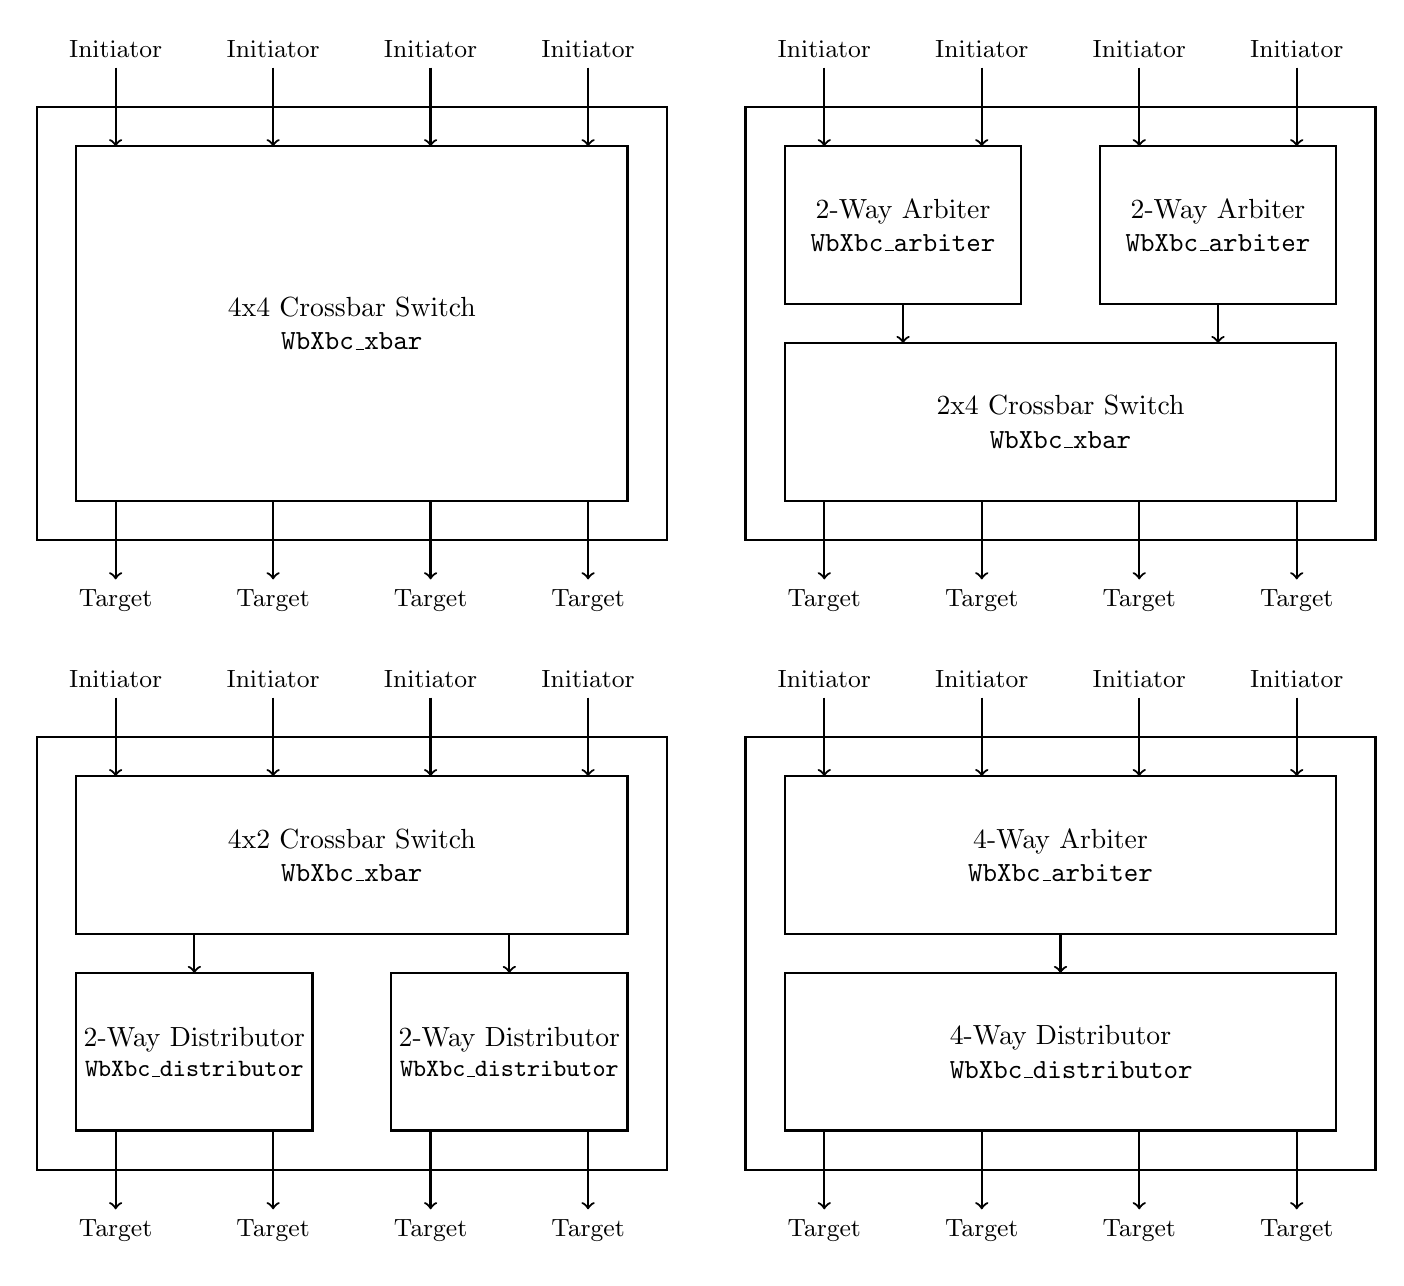
\begin{tikzpicture}

      %\draw [thin, fill=white] (0,0) rectangle (17,15.5);
      \draw[transparent] (0,0) rectangle (17,15.5);

      
      %Top level interfaces
      \newsavebox{\topif}
      \savebox{\topif}{
        \draw [thick, fill=white] (0,1) rectangle (8,6.5);
        \foreach \xpos in {1, 3, 5, 7} {
          \node [above] at (\xpos,7)  {\small{Initiator}};
          \node [below] at (\xpos,0.5){\small{Target}};
          \draw [thick, ->] (\xpos,7) -- (\xpos,6);
          \draw [thick, ->] (\xpos,1.5) -- (\xpos,0.5);
        }
      };
      %4x4 crossbar
      \node at (0,8) {\usebox{\topif}};
      %Xbar 
      \draw [thick, fill=white] (.5,9.5) rectangle (7.5,14);
      \node at (4,11.75)
            {\begin{minipage}[c]{10em}
                \begin{center}
                  \hyphenchar\font=-1
                  4x4 Crossbar Switch \\ 
                  \texttt{WbXbc\_xbar}
                \end{center}
            \end{minipage}};       
      %2x4 crossbar
      \node at (9,8) {\usebox{\topif}};
      %Arbiters
      \draw [thick, fill=white] (9.5,12) rectangle (12.5,14);
      \draw [thick, fill=white] (13.5,12) rectangle (16.5,14);
      \draw [thick, ->] (11,12) -- (11,11.5);
      \draw [thick, ->] (15,12) -- (15,11.5);
      \node at (11,13)
            {\begin{minipage}[c]{8em}
                \begin{center}
                  \hyphenchar\font=-1
                  2-Way Arbiter \\ 
                  \texttt{WbXbc\_arbiter}
                \end{center}
            \end{minipage}};       
      \node at (15,13)
            {\begin{minipage}[c]{8em}
                \begin{center}
                  \hyphenchar\font=-1
                  2-Way Arbiter \\ 
                  \texttt{WbXbc\_arbiter}
                \end{center}
            \end{minipage}};       
      %Xbar 
      \draw [thick, fill=white] (9.5,9.5) rectangle (16.5,11.5);
      \node at (13,10.5)
            {\begin{minipage}[c]{10em}
                \begin{center}
                  \hyphenchar\font=-1
                  2x4 Crossbar Switch \\ 
                  \texttt{WbXbc\_xbar}
                \end{center}
            \end{minipage}};       
      %4x2 crossbar
      \node at (0,0) {\usebox{\topif}};
      %Xbar 
      \draw [thick, fill=white] (0.5,4) rectangle (7.5,6);
      \draw [thick, ->] (2,4) -- (2,3.5);
      \draw [thick, ->] (6,4) -- (6,3.5);
      \node at (4,5)
            {\begin{minipage}[c]{10em}
                \begin{center}
                  \hyphenchar\font=-1
                  4x2 Crossbar Switch \\ 
                  \texttt{WbXbc\_xbar}
                \end{center}
            \end{minipage}};                   
      %Distributors
      \draw [thick, fill=white] (0.5,1.5) rectangle (3.5,3.5);
      \draw [thick, fill=white] (4.5,1.5) rectangle (7.5,3.5);
      \node at (2,2.5)
            {\begin{minipage}[c]{8em}
                \begin{center}
                  \hyphenchar\font=-1
                  2-Way Distributor \\ 
                  \small{\texttt{WbXbc\_distributor}}
                \end{center}
            \end{minipage}};       
      \node at (6,2.5)
            {\begin{minipage}[c]{8em}
                \begin{center}
                  \hyphenchar\font=-1
                  2-Way Distributor \\ 
                  \small{\texttt{WbXbc\_distributor}}
                \end{center}
            \end{minipage}};       
      %no crossbar
      \node at (9,0) {\usebox{\topif}};
      %Arbiter
      \draw [thick, fill=white] (9.5,4) rectangle (16.5,6);
      \draw [thick, ->] (13,4) -- (13,3.5);
      \node at (13,5)
            {\begin{minipage}[c]{8em}
                \begin{center}
                  \hyphenchar\font=-1
                  4-Way Arbiter \\ 
                  \texttt{WbXbc\_arbiter}
                \end{center}
            \end{minipage}};       
      %Distributor
      \draw [thick, fill=white] (9.5,1.5) rectangle (16.5,3.5);
      \node at (13,2.5)
            {\begin{minipage}[c]{8em}
                \begin{center}
                  \hyphenchar\font=-1
                  4-Way Distributor \\ 
                  \texttt{WbXbc\_distributor}
                \end{center}
            \end{minipage}};       
    \end{tikzpicture}
  }
  \caption{Examples of Different Crossbar Implementations}
  \label{overview:diag}
  %\end{center}
\end{figure}


%--------------------
% WbXbc integration parameters
%--------------------
%###############################################################################
%# WbXbc - Manual - Integration Parameters                                     #
%###############################################################################
%#    Copyright 2018 Dirk Heisswolf                                            #
%#    This file is part of the WbXbc project.                                  #
%#                                                                             #
%#    WbXbc is free software: you can redistribute it and/or modify            #
%#    it under the terms of the GNU General Public License as published by     #
%#    the Free Software Foundation, either version 3 of the License, or        #
%#    (at your option) any later version.                                      #
%#                                                                             #
%#    WbXbc is distributed in the hope that it will be useful,                 #
%#    but WITHOUT ANY WARRANTY; without even the implied warranty of           #
%#    MERCHANTABILITY or FITNESS FOR A PARTICULAR PURPOSE.  See the            #
%#    GNU General Public License for more details.                             #
%#                                                                             #
%#    You should have received a copy of the GNU General Public License        #
%#    along with WbXbc.  If not, see <http:%www.gnu.org/licenses/>.            #
%###############################################################################
%# Version History:                                                            #
%#   September 10, 2018                                                        #
%#      - Initial release                                                      #
%###############################################################################

\section{Integration Parameters}
\label{param}

This section specifies the integration parameters to configure the WbXbc components.
Each WbXbc component supports a subset of the parameters listed below.

\begin{description}[style=nextline]

\item[\texttt{ITR\_CNT}]
The number of initiator bus interfaces to be offered by the WbXbc component

\item[\texttt{TGT\_CNT}] 
The number of target bus interfaces to be offered by the WbXbc component

\item[\texttt{ADR\_WIDTH}] 
Width of all address busses (\texttt{ADR\_I} and \texttt{ADR\_0})

\item[\texttt{ITR\_ADR\_WIDTH}] 
Width of the initiator address bus(ses) (\texttt{ADR\_I}), in case it differs
from the target address bus(es) (\texttt{ADR\_O}) 

\item[\texttt{SEL\_WIDTH}] 
Number data select lines of all initiator and target busses
(\texttt{SEL\_I} and \texttt{SEL\_O})  

\item[\texttt{ITR\_SEL\_WIDTH}] 
Number of data select lines of the initiator bus (\texttt{SEL\_I}), in case it
from the target bus (\texttt{SEL\_O}) 

\item[\texttt{DAT\_WIDTH}] 
Width of all data busses (initiator and target, read and write direction) 

\item[\texttt{ITR\_DAT\_WIDTH}] 
Width of the initiator's data busses (read and write direction

\item[\texttt{TGA\_WIDTH}] 
Number of tags associated with the address busses of the initiator and
the target (\texttt{TGA\_I} and \texttt{TGA\_O}) 

\item[\texttt{TGC\_WIDTH}] 
Number of tags associated with the cycle indicators (\texttt{CYC\_I} and \texttt{CYC\_O}) of
thw initiator and the target (\texttt{TGC\_I} and \texttt{TGC\_O})

\item[\texttt{TGRD\_WIDTH}] 
Number of tags assoociated with the read data busses of the initiator and
the target (\texttt{TGD\_O} and \texttt{TGD\_I}) 

\item[\texttt{TGWD\_WIDTH}] 
Number of tags associated with the write data busses of the initiator and
the target (\texttt{TGD\_I} and \texttt{TGD\_O}) 

\item[\texttt{BIG\_ENDIAN}] 
Selects the endianess of the design (1=big endian, 0=little endian)

\end{description}


%--------------------
% WbXbc interface signals
%--------------------
%###############################################################################
%# WbXbc - Manual - Interface Signals                                          #
%###############################################################################
%#    Copyright 2018 Dirk Heisswolf                                            #
%#    This file is part of the WbXbc project.                                  #
%#                                                                             #
%#    WbXbc is free software: you can redistribute it and/or modify            #
%#    it under the terms of the GNU General Public License as published by     #
%#    the Free Software Foundation, either version 3 of the License, or        #
%#    (at your option) any later version.                                      #
%#                                                                             #
%#    WbXbc is distributed in the hope that it will be useful,                 #
%#    but WITHOUT ANY WARRANTY; without even the implied warranty of           #
%#    MERCHANTABILITY or FITNESS FOR A PARTICULAR PURPOSE.  See the            #
%#    GNU General Public License for more details.                             #
%#                                                                             #
%#    You should have received a copy of the GNU General Public License        #
%#    along with WbXbc.  If not, see <http://www.gnu.org/licenses/>.           #
%###############################################################################
%# Version History:                                                            #
%#   September 10, 2018                                                        #
%#      - Initial release                                                      #
%###############################################################################

\section{Interface Signals}
\label{sig}

All WbXbc components share common interface signals, which are described in this
chapter. Most of these signals refer directly to the Wishbone specification~\cite{wishbone}.

Some WbXbc components offer multiple of instances of a particular interface type (e.g. the
WbXbx Splitter offers multiple Wishbone target interfaces, the WbXbc Arbiter offers multiple
Wishbone initiator interfaces). In these cases, the interfaces are concatinated on a signal
by signal basis.
For instance, a set of concatinated Wishbone initiator interfaces shares a single
\texttt{itr\_adr\_i} bus signal. The individual bus signals are concatinated as a whole
(see \figref{sig:concat}).
The order of the signal concatination is consistent throughout all interface signals.

\begin{figure}[!h]
  %\begin{center}
  \makebox[\textwidth][c]{
    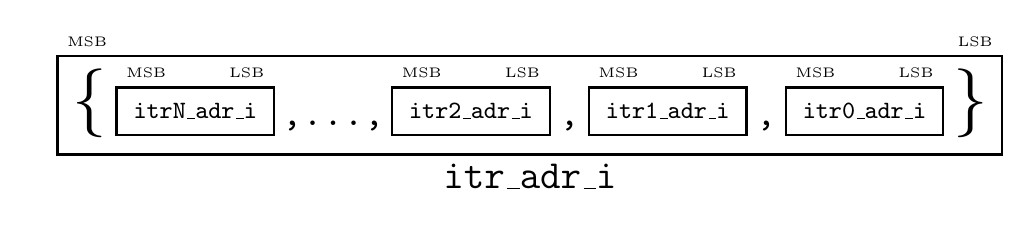
\begin{tikzpicture}
      \node [left] at (1,1.4) {\Huge{\texttt{ \{ }}};
      
      \draw [thick] (1,1) rectangle (3,1.6);
      \node at (2,1.3) {\small{\texttt{itrN\_adr\_i}}};
      \node [above right] at (1,1.6) {\tiny{MSB}};
      \node [above left]  at (3,1.6) {\tiny{LSB}};

      \node [below] at (3.75,1.3) {\Large{\texttt{,...,}}};
     
      \draw [thick] (4.5,1) rectangle (6.5,1.6);
      \node at (5.5,1.3) {\small{\texttt{itr2\_adr\_i}}};
      \node [above right] at (4.5,1.6) {\tiny{MSB}};
      \node [above left]  at (6.5,1.6) {\tiny{LSB}};

      \node [below] at (6.75,1.3) {\Large{\texttt{,}}};

      \draw [thick] (7,1) rectangle (9,1.6);
      \node at (8,1.3) {\small{\texttt{itr1\_adr\_i}}};
      \node [above right] at (7,1.6) {\tiny{MSB}};
      \node [above left]  at (9,1.6) {\tiny{LSB}};

      \node [below] at (9.25,1.3) {\Large{\texttt{,}}};

      \draw [thick] (9.5,1) rectangle (11.5,1.6);
      \node at (10.5,1.3) {\small{\texttt{itr0\_adr\_i}}};
      \node [above right] at (9.5,1.6) {\tiny{MSB}};
      \node [above left]  at (11.5,1.6) {\tiny{LSB}};

      \node [right] at (11.5,1.4) {\Huge{\texttt{\} }}};

      \draw [thick] (0.25,0.75) rectangle (12.25,2);
      \node [above right] at (0.25,2) {\tiny{MSB}};
      \node [above left]  at (12.25,2) {\tiny{LSB}};

      \node [below] at (6.25,0.75) {\Large{\texttt{itr\_adr\_i}}};
    \end{tikzpicture}
    }
    \caption{Concatination of Interface signals}
    \label{sig:concat}
  %\end{center}
\end{figure}

\subsection{Address Region Descriptors}

\begin{description}[style=nextline]
  
\item[\texttt{region\_adr\_i}] Target region descriptors (base addresses). \\
  
  The address range of each bus target is determined by a base address and an address mask.
  An address \texttt{itr\_adr\_i} is within the range of the $n$-th bus target if 
  \begin{center}
    \texttt{itr\_adr\_i[ADR\_WIDTH-1:0] |
      region\_msk\_i[(ADR\_WIDTH*($n$+1))-1:ADR\_WIDTH*$n$]} \\
    $\equiv$ \\
    \texttt{region\_adr\_i[(ADR\_WIDTH*($n$+1))-1:ADR\_WIDTH*$n$] |
      region\_msk\_i[(ADR\_WIDTH*($n$+1))-1:ADR\_WIDTH*$n$]} \\
  \end{center}

\item[\texttt{region\_msk\_i}]  Target region descriptors (address masks). \\
  See \texttt{region\_adr\_i}. 
   
\end{description}

\subsection{General Signals (SYSCON)}

\begin{description}[style=nextline]

\item[\texttt{clk\_i}] Common clock input for all Wishbone interfaces.\\  
  This clock input  corresponds to signal \texttt{CLK\_I} of the Wishbone specification~\cite{wishbone}.

\item[\texttt{itr\_clk\_i}] Clock input for all initiator busses. \\
  Target busses must be clocked by synchronous and subdivided clock.
  This clock input corresponds to signal \texttt{CLK\_I} of the Wishbone specification~\cite{wishbone}.

\item[\texttt{tgt\_clk\_i}] Clock input for all target busses. \\
  Initiator busses must be clocked by synchronous and subdivided clock.
  This clock input corresponds to signal \texttt{CLK\_I} of the Wishbone specification~\cite{wishbone}.

\item[\texttt{itr2tgt\_sync\_i}] Clock phase indicator for for the \nameref{decel} component. \\
    This signal indicates a common positive clock edge of the initiator clock and the synchronous and subdivided
    target clock (see \figref{sig:itr2tgtsync:fig}). 

  \begin{figure}[H]
    \begin{center}
      \begin{tikztimingtable}[timing/slope=0.8]
        \texttt{itr\_clk\_i}      & 15{4c}  \\
        \texttt{tgt\_clk\_i}      & 4c7{8c} \\
        \texttt{itr2tgt\_sync\_i} & 2H7{8t} \\
        \extracode
        \vertlines[thin, dotted]{2,6,...,\twidth}
      \end{tikztimingtable}
      \caption{\texttt{itr2tgt\_sync\_i} Timing Example}
      \label{sig:itr2tgtsync:fig}
    \end{center}
  \end{figure}
  
\item[\texttt{tgt2itr\_sync\_i}] Clock phase indicator for for the \nameref{accel} component. \\
  This signal indicates a common positive clock edge of the target clock and the synchronous and subdivided
  initiator clock (see \figref{sig:tgt2itrsync:fig}).

  \begin{figure}[H]
    \begin{center}
      \begin{tikztimingtable}[timing/slope=0.8]
        \texttt{itr\_clk\_i}      &  5{12c}        \\
        \texttt{tgt\_clk\_i}      & 15{4c}         \\
        \texttt{itr2tgt\_sync\_i} &  4t8t16t8t8t2H \\
        \extracode
        \vertlines[thin, dotted]{2,6,...,\twidth}        
      \end{tikztimingtable}
      \caption{\texttt{tgt2itr\_sync\_i} Timing Example}
      \label{sig:tgt2itrsync:fig}
    \end{center}
  \end{figure}

\item[\texttt{async\_rst\_i}] Optional asynchronous reset input for all sequential logic. \\
  This reset signal may assert asynchronously, but must deassert synchronously. If no
  asynchrounous reset is implemented, this input must be tied to zero.

\item[\texttt{sync\_rst\_i}] Synchronous reset input. \\
  For WbXBC components, this synchronous reset is not required, if an asynchronous reset is provided.
  If no synchrounous reset is implemented, this input must be tied to zero.
  This reset input corresponds to signal \texttt{RST\_I} of the Wishbone specification~\cite{wishbone}.
 
\end{description}

\subsection{Initiator Bus Signals}

\begin{description}[style=nextline]

\item[\texttt{itr\_cyc\_i}] Cycle indicator input. \\
  This input signal corresponds to signal \texttt{CYC\_I} of the Wishbone specification~\cite{wishbone}.

\item[\texttt{itr\_stb\_i}] Strobe input. \\
  This input signal corresponds to signal \texttt{STB\_I} of the Wishbone specification~\cite{wishbone}.

\item[\texttt{itr\_we\_i}] Write enable input. \\
  This input signal corresponds to signal \texttt{WE\_I} of the Wishbone specification~\cite{wishbone}.

\item[\texttt{itr\_lock\_i}] Cycle lock input. \\   
  This input signal corresponds to signal \texttt{LOCK\_I} of the Wishbone specification~\cite{wishbone}.
    
\item[\texttt{itr\_sel\_i}] Write data select inputs. \\
  These input signals correspond to bus \texttt{SEL\_I} of the Wishbone specification~\cite{wishbone}.
    
\item[\texttt{itr\_adr\_i}] Address bus. \\
  These input signals correspond to bus \texttt{ADR\_I} of the Wishbone specification~\cite{wishbone}.

\item[\texttt{itr\_dat\_i}] Write data bus. \\
  These input signals correspond to bus \texttt{DAT\_I} of the Wishbone specification~\cite{wishbone}.

\item[\texttt{itr\_tga\_i}] Address bus tags. \\
  These input signals correspond to bus \texttt{TGA\_I} of the Wishbone specification~\cite{wishbone}.

\item[\texttt{itr\_tgc\_i}] Cycle tags. \\
  These input signals correspond to bus \texttt{TGC\_I} of the Wishbone specification~\cite{wishbone}.

\item[\texttt{itr\_tgd\_i}] Write data tags. \\
  These input signals correspond to bus \texttt{TGD\_I} of the Wishbone specification~\cite{wishbone}.

\item[\texttt{itr\_ack\_o}] Acknowlede output. \\
  This output signal corresponds to signal \texttt{ACK\_O} of the Wishbone specification~\cite{wishbone}.
 
\item[\texttt{itr\_err\_o}] Error indicator output. \\
  This output signal corresponds to signal \texttt{ERR\_O} of the Wishbone specification~\cite{wishbone}.

\item[\texttt{itr\_rty\_o}] Retry output. \\
  This output signal corresponds to signal \texttt{RTY\_O} of the Wishbone specification~\cite{wishbone}.
  For all WbXbc components this signal serves as indicator for a lost bus arbitration.

\item[\texttt{itr\_stall\_o}] Pipeline stall output. \\
  This output signal corresponds to signal \texttt{STALL\_O} of the Wishbone specification~\cite{wishbone}.

\item[\texttt{itr\_dat\_o}] Read data bus. \\
  These output signals correspond to bus \texttt{DAT\_O} of the Wishbone specification~\cite{wishbone}.

\item[\texttt{itr\_tgd\_o}] Read data tags. \\
  These output signals correspond to bus \texttt{TGD\_O} of the Wishbone specification~\cite{wishbone}.

\end{description}

\subsection{Target Bus Signals}

\begin{description}[style=nextline]

\item[\texttt{tgt\_cyc\_o}] Cycle indicator output. \\
  This output signal corresponds to signal \texttt{CYC\_O} of the Wishbone specification~\cite{wishbone}.

\item[\texttt{tgt\_stb\_o}] Strobe output. \\   
  This output signal corresponds to signal \texttt{STB\_O} of the Wishbone specification~\cite{wishbone}.

\item[\texttt{tgt\_we\_o}]  Write enable output. \\
  This output signal corresponds to signal \texttt{WE\_O} of the Wishbone specification~\cite{wishbone}.

\item[\texttt{tgt\_lock\_o}]  Cycle lock output. \\
  This output signal corresponds to signal \texttt{LOCK\_O} of the Wishbone specification~\cite{wishbone}.

\item[\texttt{tgt\_sel\_o}] Write data select outputs. \\    
  These output signals correspond to bus \texttt{SEL\_O} of the Wishbone specification~\cite{wishbone}.

\item[\texttt{tgt\_adr\_o}] Address bus. \\   
  These output signals correspond to bus \texttt{ADR\_O} of the Wishbone specification~\cite{wishbone}.

\item[\texttt{tgt\_dat\_o}] Write data bus. \\    
  These output signals correspond to bus \texttt{DAT\_O} of the Wishbone specification~\cite{wishbone}.

\item[\texttt{tgt\_tga\_o}] Address bus tags. \\   
  These output signals correspond to bus \texttt{TGA\_O} of the Wishbone specification~\cite{wishbone}.

\item[\texttt{tgt\_tgc\_o}] Cycle tags. \\    
  These output signals correspond to bus \texttt{TGC\_O} of the Wishbone specification~\cite{wishbone}.

\item[\texttt{tgt\_tgd\_o}] Write data tags. \\  
  These output signals correspond to bus \texttt{TGD\_O} of the Wishbone specification~\cite{wishbone}.

\item[\texttt{tgt\_ack\_i}] Acknowlede input. \\   
  This input signal corresponds to signal \texttt{ACK\_I} of the Wishbone specification~\cite{wishbone}.

\item[\texttt{tgt\_err\_i}] Error indicator input. \\  
  This input signal corresponds to signal \texttt{ERR\_I} of the Wishbone specification~\cite{wishbone}.

\item[\texttt{tgt\_rty\_i}] Retry input. \\  
  This output signal corresponds to signal \texttt{RTY\_I} of the Wishbone specification~\cite{wishbone}.
  For all WbXbc components this signal serves as indicator for a lost bus arbitration.

\item[\texttt{tgt\_stall\_i}] Pipeline stall input. \\
  This input signal corresponds to signal \texttt{STALL\_I} of the Wishbone specification~\cite{wishbone}.

\item[\texttt{tgt\_dat\_i}] Read data bus. \\ 
  These input signals correspond to bus \texttt{DAT\_I} of the Wishbone specification~\cite{wishbone}.

\item[\texttt{tgt\_tgd\_i}] Read data tags. \\
  These input signals correspond to bus \texttt{TGD\_I} of the Wishbone specification~\cite{wishbone}.

\end{description}



%--------------------
% WbXbc components
%--------------------
%###############################################################################
%# WbXbc - Manual - Crossbar Switch components                                 #
%###############################################################################
%#    Copyright 2018 Dirk Heisswolf                                            #
%#    This file is part of the WbXbc project.                                  #
%#                                                                             #
%#    WbXbc is free software: you can redistribute it and/or modify            #
%#    it under the terms of the GNU General Public License as published by     #
%#    the Free Software Foundation, either version 3 of the License, or        #
%#    (at your option) any later version.                                      #
%#                                                                             #
%#    WbXbc is distributed in the hope that it will be useful,                 #
%#    but WITHOUT ANY WARRANTY; without even the implied warranty of           #
%#    MERCHANTABILITY or FITNESS FOR A PARTICULAR PURPOSE.  See the            #
%#    GNU General Public License for more details.                             #
%#                                                                             #
%#    You should have received a copy of the GNU General Public License        #
%#    along with WbXbc.  If not, see <http://www.gnu.org/licenses/>.           #
%###############################################################################
%# Version History:                                                            #
%#   September 10, 2018                                                        #
%#      - Initial release                                                      #
%###############################################################################

\section{Crossbar Switch components}

TBD



%###############################################################################
%# WbXbc - Manual - Address Bus Decoder                                        #
%###############################################################################
%#    Copyright 2018 Dirk Heisswolf                                            #
%#    This file is part of the WbXbc WbXbc.                                  #
%#                                                                             #
%#    project is free software: you can redistribute it and/or modify            #
%#    it under the terms of the GNU General Public License as published by     #
%#    the Free Software Foundation, either version 3 of the License, or        #
%#    (at your option) any later version.                                      #
%#                                                                             #
%#    WbXbc is distributed in the hope that it will be useful,                 #
%#    but WITHOUT ANY WARRANTY; without even the implied warranty of           #
%#    MERCHANTABILITY or FITNESS FOR A PARTICULAR PURPOSE.  See the            #
%#    GNU General Public License for more details.                             #
%#                                                                             #
%#    You should have received a copy of the GNU General Public License        #
%#    along with WbXbc.  If not, see <http://www.gnu.org/licenses/>.           #
%###############################################################################
%# Version History:                                                            #
%#   September 10, 2018                                                        #
%#      - Initial release                                                      #
%###############################################################################

\subsection[WbXbc Address Decoder]{WbXbc Address Decoder (\texttt{WbXbc\_addesss\_decoder})}
\label{adec}

This module implements an address decoder for the Wishbone protocol. It 
propagates accesses from the initiator bus to the target bus and adds a 
set of address tags which selecting the target block (see \figref{adec:diag}).                   
%               +-------------------+                
%   Address     |                   |                
%   Regions --->|                   |                
%               |      WbXbc        |     Target  
%   Initiator   |      Address      +---> Bus    
%   Bus     --->|      Decoder      |     with   
%   w/out       |                   |     Selects 
%   Selects     |                   |                
%               +-------------------+                 
\begin{figure}[!h]
  \begin{center}
    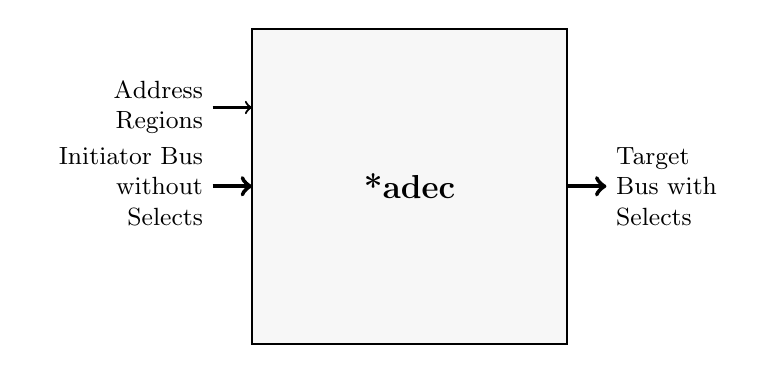
\begin{tikzpicture}
      %Block
      \draw [thick, fill=gray!6] (4,0) rectangle (8,4);
      \node at (6,2)
            {\begin{minipage}[c]{8em}
                \begin{center}
                  \hyphenchar\font=-1
                  \large{\textbf{\nameref*{adec}}}
                \end{center}
             \end{minipage}};
      %Inputs     
      \node [left] at (3.5,3)
            {\begin{minipage}[c]{6em}
                \begin{flushright}
                  \hyphenchar\font=-1
                  \small{Address Regions}
                \end{flushright}
             \end{minipage}};
      \draw [thick, ->] (3.5,3) -- (4,3);
      \node [left] at (3.5,2)
            {\begin{minipage}[c]{6em}
                \begin{flushright}
                  \hyphenchar\font=-1
                  \small{Initiator Bus without Selects}
                \end{flushright}
             \end{minipage}};
      \draw [ultra thick, ->] (3.5,2) -- (4,2);
      %Outputs     
      \node [right] at (8.5,2)
            {\begin{minipage}[c]{4em}
                \begin{flushleft}
                  \hyphenchar\font=-1
                  \small{Target Bus with Selects}
                \end{flushleft}
             \end{minipage}};
      \draw [ultra thick, ->] (8,2) -- (8.5,2);
    \end{tikzpicture}
    \caption{Block Diagram of the \nameref*{adec}}
    \label{adec:diag}
  \end{center}
\end{figure}

\subsubsection{Integration Parameters}
\label{adec:param}

The \nameref*{adec} supports the integration parameters listed in \tabref{adec:param:tab}. 
See \secref{param} for a detailed description of all integration parameters.

\begin{center}
  \rowcolors{1}{gray!12}{white}                                         %set alternating row color
  \begin{longtable}{|l|r|l|}
    \rowcolor{white}
    \caption{Integration Parameters of the \nameref*{adec}}
    \label{adec:param:tab} \\
    %Header
    \hline                                     
    \rowcolor{gray!25}
    \multicolumn{1}{|c|}{\textbf{\rule{0pt}{2.5ex} Parameter}}  &  
    \multicolumn{1}{c|}{\textbf{\rule{0pt}{2.5ex}  Default}}    & 
    \multicolumn{1}{c|}{\textbf{\rule{0pt}{2.5ex}  Decription}} \\
    \hline                                    
    \endhead                               
    %Footers
    \hline
    \rowcolor{white}
    \multicolumn{3}{r}{\tiny{...continued}} \\
    \endfoot
    \hline
    \endlastfoot
    %Content
    \texttt{TGT\_CNT   } & \texttt{4}  & Number of target addresses to decode \\
    \texttt{ADR\_WIDTH} & \texttt{16}  & Width of the address bus             \\
    \texttt{DAT\_WIDTH} & \texttt{16}  & Width of each data bus               \\
    \texttt{SEL\_WIDTH } & \texttt{2}  & Number of data select lines          \\
    \texttt{TGA\_WIDTH } & \texttt{1}  & Number of address tags               \\
    \texttt{TGC\_WIDTH } & \texttt{1}  & Number of cycle tags                 \\
    \texttt{TGRD\_WIDTH} & \texttt{1}  & Number of read data tags             \\
    \texttt{TGWD\_WIDTH} & \texttt{1}  & Number of write data tags            \\
  \end{longtable}
\end{center}

\subsubsection{Interface Signals}
\label{adec:sig}

\tabref{adec:sig:tab} lists the interface signals of the \nameref*{adec}. 
See \secref{sig} for a detailed description of all interface signals.

\begingroup
\setlength{\LTleft}{-20cm plus -1fill}
\setlength{\LTright}{\LTleft}
\begin{center}
  \rowcolors{1}{gray!12}{white}                                         %set alternating row color
  \begin{longtable}{|l|r|l|l|}
    \rowcolor{white}
    \caption{Interface Signals of the \nameref*{adec}}
    \label{adec:sig:tab} \\
    %Header
    \hline                                     
    \rowcolor{gray!25}
    \multicolumn{1}{|c|}{\textbf{\rule{0pt}{2.5ex} Signal}}     &  
    \multicolumn{1}{c|}{\textbf{\rule{0pt}{2.5ex}  Range}}      & 
    \multicolumn{1}{c|}{\textbf{\rule{0pt}{2.5ex}  Direction}}  & 
    \multicolumn{1}{c|}{\textbf{\rule{0pt}{2.5ex}  Decription}} \\
    \hline
    \endhead                               
    %Footers
    \hline
    \rowcolor{white}
    \multicolumn{4}{r}{\tiny{...continued}} \\
    \endfoot
    \hline
    \endlastfoot
    %Section 'Target Address Regions'
    %\hline
    \rowcolor{gray!20}
    \multicolumn{4}{|c|}{\scriptsize{\rule{0pt}{2.5ex} Target Address Regions}} \global\rownum=1\relax \\  
    \hline                                    
    \texttt{region\_adr\_i} & \texttt{(TGT\_CNT*ADR\_WIDTH)\-1:0} & input & target address regions                     \\
    \texttt{region\_msk\_i} & \texttt{(TGT\_CNT*ADR\_WIDTH)\-1:0} & input & \makecell[l]{selects relevant address bits \\
                                                                                          1: relevant, 0: ignored)}    \\
    %Section 'Initiator Interface'
    \hline                                 
    \rowcolor{gray!20}
    \multicolumn{4}{|c|}{\scriptsize{\rule{0pt}{2.5ex} Initiator Interface}} \global\rownum=1\relax \\    
    \hline                                 
    \texttt{itr\_cyc\_i}   &                                & input  & bus cycle indicator       \\
    \texttt{itr\_stb\_i}   &                                & input  & access request            \\
    \texttt{itr\_we\_i}    &                                & input  & write enable              \\
    \texttt{itr\_lock\_i}  &                                & input  & uninterruptable bus cycle \\
    \texttt{itr\_sel\_i}   & \texttt{SEL\_WIDTH-1:0}        & input  & write data selects        \\
    \texttt{itr\_adr\_i}   & \texttt{ADR\_WIDTH-1:0}        & input  & address bus               \\
    \texttt{itr\_dat\_i}   & \texttt{DAT\_WIDTH-1:0}        & input  & write data bus            \\
    \texttt{itr\_tga\_i}   & \texttt{TGA\_WIDTH-1:0}        & input  & address tags              \\
    \texttt{itr\_tgc\_i}   & \texttt{TGC\_WIDTH-1:0}        & input  & bus cycle tags            \\
    \texttt{itr\_tgd\_i}   & \texttt{TGWD\_WIDTH-1:0}       & input  & write data tags           \\
    \texttt{itr\_ack\_o}   &                                & output & bus cycle acknowledge     \\
    \texttt{itr\_err\_o}   &                                & output & error indicator           \\
    \texttt{itr\_rty\_o}   &                                & output & retry request             \\
    \texttt{itr\_stall\_o} &                                & output & access delay              \\
    \texttt{itr\_dat\_o}   & \texttt{DAT\_WIDTH-1:0}        & output & read data bus             \\
    \texttt{itr\_tgd\_o}   & \texttt{TGRD\_WIDTH-1:0}       & output & read data tags            \\ 
    %Section 'Target Interface'
    \hline                                                                                      
    \rowcolor{gray!20}
    \multicolumn{4}{|c|}{\scriptsize{\rule{0pt}{2.5ex} Target Interface}} \global\rownum=1\relax \\  
    \hline                                                                                      
    \texttt{tgt\_cyc\_o}         &                          & output & bus cycle indicator       \\
    \texttt{tgt\_stb\_o}         &                          & output & access request            \\
    \texttt{tgt\_we\_o}          &                          & output & write enable              \\
    \texttt{tgt\_lock\_o}        &                          & output & uninterruptable bus cycle \\
    \texttt{tgt\_sel\_o}         & \texttt{SEL\_WIDTH-1:0}  & output & write data selects        \\
    \texttt{tgt\_adr\_o}         & \texttt{ADR\_WIDTH-1:0}  & output & write data selects        \\
    \texttt{tgt\_dat\_o}         & \texttt{DAT\_WIDTH-1:0 } & output & write data bus            \\
    \texttt{tgt\_tga\_o}         & \texttt{TGA\_WIDTH-1:0}  & output & address tags              \\
    \texttt{itr\_tga\_tgtsel\_o} & \texttt{TGT\_CNT-1:0}    & output & target select tags        \\
    \texttt{tgt\_tgc\_o}         & \texttt{TGC\_WIDTH-1:0}  & output & bus cycle tags            \\
    \texttt{tgt\_tgd\_o}         & \texttt{TGWD\_WIDTH-1:0} & output & write data tags           \\
    \texttt{tgt\_ack\_i}         &                          & input  & bus cycle acknowledge     \\
    \texttt{tgt\_err\_i}         &                          & input  & error indicator           \\
    \texttt{tgt\_rty\_i}         &                          & input  & retry request             \\
    \texttt{tgt\_stall\_i}       &                          & input  & access delay              \\
    \texttt{tgt\_dat\_i}         & \texttt{DAT\_WIDTH-1:0}  & input  & read data bus             \\
    \texttt{tgt\_tgd\_i}         & \texttt{TGRD\_WIDTH-1:0} & input  & read data tags            \\   
  \end{longtable}
\end{center}  
\endgroup

\subsubsection{Verification Status}
\label{adec:verif}

\tabref[Table]{adec:verif:tab} provides an overview of the verification status of the \nameref*{adec}.
Lint checks have been done with the Icarus Verilog simulator~\cite{iverilog} and the Yosys synthesis tool~\cite{yosys}.

\begin{center}
  \rowcolors{1}{gray!12}{white}                                         %set alternating row color
  \begin{longtable}{|lr|c|c|c|c|}
    \rowcolor{white}
    \caption[Interface Signals]{Verification Status of the \nameref*{adec}}
    \label{adec:verif:tab} \\
    %Header
    \hline                              
    \rowcolor{gray!25}
    \multicolumn{2}{|c|}{\textbf{\rule{0pt}{2.5ex} Configuration}} &  
    \multicolumn{1}{c|}{\textbf{\rule{0pt}{2.5ex}  Linting}}       &  
    \multicolumn{1}{c|}{\textbf{\rule{0pt}{2.5ex}  Simulation}}    &  
    \multicolumn{1}{c|}{\textbf{\rule{0pt}{2.5ex}  Formal}}        &  
    \multicolumn{1}{c|}{\textbf{\rule{0pt}{2.5ex}  FPGA}}          \\
    \hline                              
    \endhead                               
    %Footers
    \hline
    \rowcolor{white}
    \multicolumn{6}{r}{\tiny{...continued}} \\
    \endfoot
    \hline
    \endlastfoot
    %Content
    \makecell[l]{\underline{\smash{\texttt{default}:}} \\ 
                 \texttt{ADR\_WIDTH}  \\
                 \texttt{DAT\_WIDTH}  \\
                 \texttt{SEL\_WIDTH}  \\
                 \texttt{TGA\_WIDTH}  \\
                 \texttt{TGC\_WIDTH}  \\
                 \texttt{TGRD\_WIDTH} \\
                 \texttt{TGWD\_WIDTH}}   &
    \makecell[r]{                     \\ 
                 \texttt{16}          \\
                 \texttt{16}          \\
                 \texttt{2}           \\
                 \texttt{1}           \\
                 \texttt{1}           \\
                 \texttt{1}           \\
                 \texttt{1}}             &     
    \makecell[c]{iVerilog~\cite{iverilog} \\                    
                 Yosis~\cite{yosys}}     &
    & & \\
  \end{longtable}
\end{center}
  


%###############################################################################
%# WbXbc - Manual - Error Generator                                            #
%###############################################################################
%#    Copyright 2018 Dirk Heisswolf                                            #
%#    This file is part of the WbXbc project.                                  #
%#                                                                             #
%#    WbXbc is free software: you can redistribute it and/or modify            #
%#    it under the terms of the GNU General Public License as published by     #
%#    the Free Software Foundation, either version 3 of the License, or        #
%#    (at your option) any later version.                                      #
%#                                                                             #
%#    WbXbc is distributed in the hope that it will be useful,                 #
%#    but WITHOUT ANY WARRANTY; without even the implied warranty of           #
%#    MERCHANTABILITY or FITNESS FOR A PARTICULAR PURPOSE.  See the            #
%#    GNU General Public License for more details.                             #
%#                                                                             #
%#    You should have received a copy of the GNU General Public License        #
%#    along with WbXbc.  If not, see <http://www.gnu.org/licenses/>.           #
%###############################################################################
%# Version History:                                                            #
%#   September 20, 2018                                                        #
%#      - Initial release                                                      #
%###############################################################################

\subsection[WbXbc Error Generator]{WbXbc Error Generator (\texttt{WbXbc\_error\_generator})}
\label{errgen}

This module implements an error generator or dummy target for the      
pipelined Wishbone protocol. It propagates accesses from the initiator 
to the target bus, but intercepts accesses without a target, signaling 
an error condition to the initiator. The target association is         
determined by a set of address tags, generated by the address decoder
(see \figref{errgen:diag}).                   
%             +-------------------+            
%             |                   |            
%             |                   |            
% Initiator   |     WbXbc         |     Target  
% Bus     --->|     Error         +---> Bus    
% with        |     Generator     |     with   
% Selects     |                   |     Selects 
%             |                   |            
%             +-------------------+            
\begin{figure}[!h]
  \begin{center}
    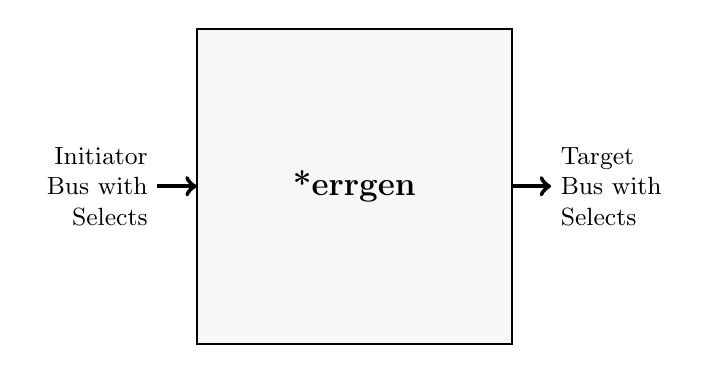
\begin{tikzpicture}
      %Block
      \draw [thick, fill=gray!6] (4,0) rectangle (8,4);
      \node at (6,2)
            {\begin{minipage}[c]{8em}
                \begin{center}
                  \hyphenchar\font=-1
                  \large{\textbf{\nameref*{errgen}}}
                \end{center}
             \end{minipage}};
      %Inputs     
      \node [left] at (3.5,2)
            {\begin{minipage}[c]{4em}
                \begin{flushright}
                  \hyphenchar\font=-1
                  \small{Initiator Bus with Selects}
                \end{flushright}
             \end{minipage}};
      \draw [ultra thick, ->] (3.5,2) -- (4,2);
      %Outputs     
      \node [right] at (8.5,2)
            {\begin{minipage}[c]{4em}
                \begin{flushleft}
                  \hyphenchar\font=-1
                  \small{Target Bus with Selects}
                \end{flushleft}
             \end{minipage}};
      \draw [ultra thick, ->] (8,2) -- (8.5,2);
    \end{tikzpicture}
    \caption{Block Diagram of the \nameref*{errgen}}
    \label{errgen:diag}
  \end{center}
\end{figure}

\subsubsection{Integration Parameters}
\label{errgen:param}

The \nameref*{errgen} supports the integration parameters listed in \tabref{errgen:param:tab}. 
See \secref{param} for a detailed description of all integration parameters.

\begin{center}
  \rowcolors{1}{gray!12}{white}                                         %set alternating row color
  \begin{longtable}{|l|r|l|}
    \rowcolor{white}
    \caption{Integration Parameters of the \nameref*{errgen}}
    \label{errgen:param:tab} \\
    %Header
    \hline                                     
    \rowcolor{gray!25}
    \multicolumn{1}{|c|}{\textbf{\rule{0pt}{2.5ex} Parameter}}  &  
    \multicolumn{1}{c|}{\textbf{\rule{0pt}{2.5ex}  Default}}    & 
    \multicolumn{1}{c|}{\textbf{\rule{0pt}{2.5ex}  Decription}} \\
    \hline                                    
    \endhead                               
    %Footers
    \hline
    \rowcolor{white}
    \multicolumn{3}{r}{\tiny{...continued}} \\
    \endfoot
    \hline
    \endlastfoot
    %Content
    \texttt{TGT\_CNT   } & \texttt{4}  & Number of target addresses to decode \\
    \texttt{ADR\_WIDTH} & \texttt{16} & Width of the address bus              \\
    \texttt{DAT\_WIDTH} & \texttt{16} & Width of each data bus                \\
    \texttt{SEL\_WIDTH } & \texttt{2}  & Number of data select lines          \\
    \texttt{TGA\_WIDTH } & \texttt{1}  & Number of address tags               \\
    \texttt{TGC\_WIDTH } & \texttt{1}  & Number of cycle tags                 \\
    \texttt{TGRD\_WIDTH} & \texttt{1}  & Number of read data tags             \\
    \texttt{TGWD\_WIDTH} & \texttt{1}  & Number of write data tags            \\
  \end{longtable}
\end{center}

\pagebreak

\subsubsection{Interface Signals}
\label{errgen:sig}

\tabref{errgen:sig:tab} lists the interface signals of the \nameref*{errgen}. 
See \secref{sig} for a detailed description of all interface signals.

\begin{center}
  \rowcolors{1}{gray!12}{white}                                         %set alternating row color
  \begin{longtable}{|l|r|l|l|}
    \rowcolor{white}
    \caption{Interface Signals of the \nameref*{errgen}}
    \label{errgen:sig:tab} \\
    %Header
    \hline                                     
    \rowcolor{gray!25}
    \multicolumn{1}{|c|}{\textbf{\rule{0pt}{2.5ex} Signal}}     &  
    \multicolumn{1}{c|}{\textbf{\rule{0pt}{2.5ex}  Range}}      & 
    \multicolumn{1}{c|}{\textbf{\rule{0pt}{2.5ex}  Direction}}  & 
    \multicolumn{1}{c|}{\textbf{\rule{0pt}{2.5ex}  Decription}} \\
    \hline
    \endhead                               
    %Footers
    \hline
    \rowcolor{white}
    \multicolumn{4}{r}{\tiny{...continued}} \\
    \endfoot
    \hline
    \endlastfoot
    %Section 'Clock and Reset'
    %\hline
    \rowcolor{gray!20}
    \multicolumn{4}{|c|}{\scriptsize{\rule{0pt}{2.5ex} Clock and Reset}} \global\rownum=1\relax \\  
    \hline                                    
    \texttt{clk\_i}        &                                & input & module clock              \\
    \texttt{async\_rst\_i} &                                & input & asynchronous reset        \\
    \texttt{sync\_rst\_i}  &                                & input & synchronous reset         \\
    %Section 'Initiator Interface'
    \hline                                 
    \rowcolor{gray!20}
    \multicolumn{4}{|c|}{\scriptsize{\rule{0pt}{2.5ex} Initiator Interface}} \global\rownum=1\relax \\    
    \hline                                 
    \texttt{itr\_cyc\_i}   &                                & input  & bus cycle indicator       \\
    \texttt{itr\_stb\_i}   &                                & input  & access request            \\
    \texttt{itr\_we\_i}    &                                & input  & write enable              \\
    \texttt{itr\_lock\_i}  &                                & input  & uninterruptable bus cycle \\
    \texttt{itr\_sel\_i}   & \texttt{SEL\_WIDTH-1:0}        & input  & write data selects        \\
    \texttt{itr\_adr\_i}   & \texttt{ADR\_WIDTH-1:0}       & input  & address bus                \\
    \texttt{itr\_dat\_i}   & \texttt{DAT\_WIDTH-1:0}       & input  & write data bus             \\
    \texttt{itr\_tga\_i}   & \texttt{TGA\_WIDTH-1:0}        & input  & address tags              \\
    \texttt{itr\_tga\_tgtsel\_i} & \texttt{TGT\_CNT-1:0}    & input  & target select tags        \\
    \texttt{itr\_tgc\_i}   & \texttt{TGC\_WIDTH-1:0}        & input  & bus cycle tags            \\
    \texttt{itr\_tgd\_i}   & \texttt{TGWD\_WIDTH-1:0}       & input  & write data tags           \\
    \texttt{itr\_ack\_o}   &                                & output & bus cycle acknowledge     \\
    \texttt{itr\_err\_o}   &                                & output & error indicator           \\
    \texttt{itr\_rty\_o}   &                                & output & retry request             \\
    \texttt{itr\_stall\_o} &                                & output & access delay              \\
    \texttt{itr\_dat\_o}   & \texttt{DAT\_WIDTH-1:0}       & output & read data bus             \\
    \texttt{itr\_tgd\_o}   & \texttt{TGRD\_WIDTH-1:0}       & output & read data tags            \\ 
    %Section 'Target Interface'
    \hline                                                                                      
    \rowcolor{gray!20}
    \multicolumn{4}{|c|}{\scriptsize{\rule{0pt}{2.5ex} Target Interface}} \global\rownum=1\relax \\  
    \hline                                                                                      
    \texttt{tgt\_cyc\_o}         &                          & output & bus cycle indicator       \\
    \texttt{tgt\_stb\_o}         &                          & output & access request            \\
    \texttt{tgt\_we\_o}          &                          & output & write enable              \\
    \texttt{tgt\_lock\_o}        &                          & output & uninterruptable bus cycle \\
    \texttt{tgt\_sel\_o}         & \texttt{SEL\_WIDTH-1:0}  & output & write data selects        \\
    \texttt{tgt\_adr\_o}         & \texttt{ADR\_WIDTH-1:0} & output & write data selects         \\
    \texttt{tgt\_dat\_o}         & \texttt{DAT\_WIDTH-1:0} & output & write data bus             \\
    \texttt{tgt\_tga\_o}         & \texttt{TGA\_WIDTH-1:0}  & output & address tags              \\
    \texttt{itr\_tga\_tgtsel\_o} & \texttt{TGT\_CNT-1:0}    & output & target select tags        \\
    \texttt{tgt\_tgc\_o}         & \texttt{TGC\_WIDTH-1:0}  & output & bus cycle tags            \\
    \texttt{tgt\_tgd\_o}         & \texttt{TGWD\_WIDTH-1:0} & output & write data tags           \\
    \texttt{tgt\_ack\_i}         &                          & input  & bus cycle acknowledge     \\
    \texttt{tgt\_err\_i}         &                          & input  & error indicator           \\
    \texttt{tgt\_rty\_i}         &                          & input  & retry request             \\
    \texttt{tgt\_stall\_i}       &                          & input  & access delay              \\
    \texttt{tgt\_dat\_i}         & \texttt{DAT\_WIDTH-1:0} & input  & read data bus              \\
    \texttt{tgt\_tgd\_i}         & \texttt{TGRD\_WIDTH-1:0} & input  & read data tags            \\   
  \end{longtable}
\end{center}  

\pagebreak

\subsubsection{Verification Status}
\label{errgen:verif}

\tabref[Table]{errgen:verif:tab} provides an overview of the verification status of the \nameref*{errgen}.

\begin{center}
  \rowcolors{1}{gray!12}{white}                                         %set alternating row color
  \begin{longtable}{|lr|c|c|c|c|}
    \rowcolor{white}
    \caption[Interface Signals]{Verification Status of the \nameref*{errgen}}
    \label{errgen:verif:tab} \\
    %Header
    \hline                              
    \rowcolor{gray!25}
    \multicolumn{2}{|c|}{\textbf{\rule{0pt}{2.5ex} Configuration}} &  
    \multicolumn{1}{c|}{\textbf{\rule{0pt}{2.5ex}  Linting}}       &  
    \multicolumn{1}{c|}{\textbf{\rule{0pt}{2.5ex}  Simulation}}    &  
    \multicolumn{1}{c|}{\textbf{\rule{0pt}{2.5ex}  Formal}}        &  
    \multicolumn{1}{c|}{\textbf{\rule{0pt}{2.5ex}  FPGA}}          \\
    \hline                              
    \endhead                               
    %Footers
    \hline
    \rowcolor{white}
    \multicolumn{6}{r}{\tiny{...continued}} \\
    \endfoot
    \hline
    \endlastfoot
    %Content
    \makecell[l]{\underline{\smash{\texttt{default}:}} \\ 
                 \texttt{ADR\_WIDTH}  \\
                 \texttt{DAT\_WIDTH}  \\
                 \texttt{SEL\_WIDTH}  \\
                 \texttt{TGA\_WIDTH}  \\
                 \texttt{TGC\_WIDTH}  \\
                 \texttt{TGRD\_WIDTH} \\
                 \texttt{TGWD\_WIDTH}}   &
    \makecell[r]{                     \\ 
                 \texttt{16}          \\
                 \texttt{16}          \\
                 \texttt{2}           \\
                 \texttt{1}           \\
                 \texttt{1}           \\
                 \texttt{1}           \\
                 \texttt{1}}             &     
    \makecell[c]{Verilator~\cite{verilator} \\                    
                 iVerilog~\cite{iverilog} \\                    
                 Yosis~\cite{yosys}}     &
    & 
    \makecell[c]{SymbiYosys~\cite{sby} \\                    
                 (SMTBMC flow\footnotemark)} \footnotetext{see \secref{verification}}& \\
  \end{longtable}
\end{center}
  


%###############################################################################
%# WbXbc - Manual - Bus Splitter                                               #
%###############################################################################
%#    Copyright 2018 Dirk Heisswolf                                            #
%#    This file is part of the WbXbc project.                                  #
%#                                                                             #
%#    WbXbc is free software: you can redistribute it and/or modify            #
%#    it under the terms of the GNU General Public License as published by     #
%#    the Free Software Foundation, either version 3 of the License, or        #
%#    (at your option) any later version.                                      #
%#                                                                             #
%#    WbXbc is distributed in the hope that it will be useful,                 #
%#    but WITHOUT ANY WARRANTY; without even the implied warranty of           #
%#    MERCHANTABILITY or FITNESS FOR A PARTICULAR PURPOSE.  See the            #
%#    GNU General Public License for more details.                             #
%#                                                                             #
%#    You should have received a copy of the GNU General Public License        #
%#    along with WbXbc.  If not, see <http://www.gnu.org/licenses/>.           #
%###############################################################################
%# Version History:                                                            #
%#   September 21, 2018                                                        #
%#      - Initial release                                                      #
%###############################################################################

\subsection[WbXbc Splitter]{WbXbc Splitter (\texttt{WbXbc\_splitter})}
\label{split}

This module implements a bus splitter for the pipelined Wishbone       
protocol. Accesses from the initiator bus are propagated to one of the 
target busses. The target busses are selected by a set of address tags,
generated by the address decoder(see \figref{split:diag}).         
%             +-------------------+             
%             |                   +--->         
% Single      |                   |             
% Initiator   |      WbXbc        +---> Multiple
% Bus     --->|      Splitter     |     Target 
% with        |                   | ... Busses 
% Selects     |                   |             
%             |                   +--->         
%             +-------------------+             
\begin{figure}[!h]
  \begin{center}
    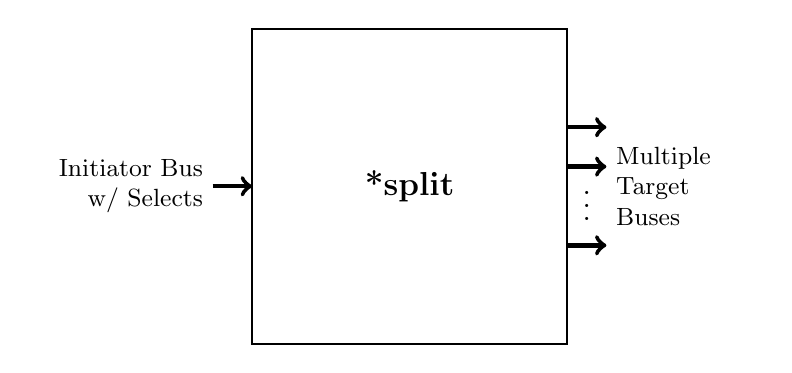
\begin{tikzpicture}
      %Block
      \draw [thick, fill=white] (4,0) rectangle (8,4);
      \node at (6,2)
            {\begin{minipage}[c]{8em}
                \begin{center}
                  \hyphenchar\font=-1
                  \large{\textbf{\nameref*{split}}}
                \end{center}
             \end{minipage}};
      %Inputs     
      \node [left] at (3.5,2)
            {\begin{minipage}[c]{6em}
                \begin{flushright}
                  \hyphenchar\font=-1
                  \small{Initiator Bus w/ Selects}
                \end{flushright}
             \end{minipage}};
      \draw [ultra thick, ->] (3.5,2) -- (4,2);
      %Outputs     
      \node [right] at (8.5,2)
            {\begin{minipage}[c]{5em}
                \begin{flushleft}
                  \hyphenchar\font=-1
                  \small{Multiple Target Buses}
                \end{flushleft}
             \end{minipage}};
      \draw [ultra thick, ->] (8,2.75) -- (8.5,2.75);
      \draw [ultra thick, ->] (8,2.25) -- (8.5,2.25);
      \node [rotate=90] at (8.25,1.75) {\small{\texttt{...}}};
      \draw [ultra thick, ->] (8,1.25) -- (8.5,1.25);
    \end{tikzpicture}
    \caption{Block Diagram of the \nameref*{split}}
    \label{split:diag}
  \end{center}
\end{figure}
  

\subsubsection{Integration Parameters}
\label{split:param}

The \nameref*{split} supports the integration parameters listed in \tabref{split:param:tab}. 
See \secref{param} for a detailed description of all integration parameters.

\begin{center}
  \rowcolors{1}{gray!12}{white}                                         %set alternating row color
  \begin{longtable}{|l|r|l|}
    \rowcolor{white}
    \caption{Integration Parameters of the \nameref*{split}}
    \label{split:param:tab} \\
    %Header
    \hline                                     
    \rowcolor{gray!25}
    \multicolumn{1}{|c|}{\textbf{\rule{0pt}{2.5ex} Parameter}}  &  
    \multicolumn{1}{c|}{\textbf{\rule{0pt}{2.5ex}  Default}}    & 
    \multicolumn{1}{c|}{\textbf{\rule{0pt}{2.5ex}  Decription}} \\
    \hline                                    
    \endhead                               
    %Footers
    \hline
    \rowcolor{white}
    \multicolumn{3}{r}{\tiny{...continued}} \\
    \endfoot
    \hline
    \endlastfoot
    %Content
    \texttt{TGT\_CNT   } & \texttt{4}  & Number of target addresses to decode \\
    \texttt{ADDR\_WIDTH} & \texttt{16} & Width of the address bus             \\
    \texttt{DATA\_WIDTH} & \texttt{16} & Width of each data bus               \\
    \texttt{SEL\_WIDTH } & \texttt{2}  & Number of data select lines          \\
    \texttt{TGA\_WIDTH } & \texttt{1}  & Number of address tags               \\
    \texttt{TGC\_WIDTH } & \texttt{1}  & Number of cycle tags                 \\
    \texttt{TGRD\_WIDTH} & \texttt{1}  & Number of read data tags             \\
    \texttt{TGWD\_WIDTH} & \texttt{1}  & Number of write data tags            \\
  \end{longtable}
\end{center}

\subsubsection{Interface Signals}
\label{split:sig}

\tabref{split:sig:tab} lists the interface signals of the \nameref*{split}. 
See \secref{sig} for a detailed description of all interface signals.

\begin{center}
  \rowcolors{1}{gray!12}{white}                                         %set alternating row color
  \begin{longtable}{|l|r|l|l|}
    \rowcolor{white}
    \caption{Interface Signals of the \nameref*{split}}
    \label{split:sig:tab} \\
    %Header
    \hline                                     
    \rowcolor{gray!25}
    \multicolumn{1}{|c|}{\textbf{\rule{0pt}{2.5ex} Signal}}     &  
    \multicolumn{1}{c|}{\textbf{\rule{0pt}{2.5ex}  Range}}      & 
    \multicolumn{1}{c|}{\textbf{\rule{0pt}{2.5ex}  Direction}}  & 
    \multicolumn{1}{c|}{\textbf{\rule{0pt}{2.5ex}  Decription}} \\
    \hline
    \endhead                               
    %Footers
    \hline
    \rowcolor{white}
    \multicolumn{4}{r}{\tiny{...continued}} \\
    \endfoot
    \hline
    \endlastfoot
    %Section 'Clock and Reset'
    %\hline
    \rowcolor{gray!20}
    \multicolumn{4}{|c|}{\scriptsize{\rule{0pt}{2.5ex} Clock and Reset}} \global\rownum=1\relax \\  
    \hline                                    
    \texttt{clk\_i}        &                                & input & module clock              \\
    \texttt{async\_rst\_i} &                                & input & asynchronous reset        \\
    \texttt{sync\_rst\_i}  &                                & input & synchronous reset         \\
    %Section 'Initiator Interface'
    \hline                                 
    \rowcolor{gray!20}
    \multicolumn{4}{|c|}{\scriptsize{\rule{0pt}{2.5ex} Initiator Interface}} \global\rownum=1\relax \\    
    \hline                                 
    \texttt{itr\_cyc\_i}   &                                & input  & bus cycle indicator       \\
    \texttt{itr\_stb\_i}   &                                & input  & access request            \\
    \texttt{itr\_we\_i}    &                                & input  & write enable              \\
    \texttt{itr\_lock\_i}  &                                & input  & uninterruptable bus cycle \\
    \texttt{itr\_sel\_i}   & \texttt{SEL\_WIDTH-1:0}        & input  & write data selects        \\
    \texttt{itr\_adr\_i}   & \texttt{ADDR\_WIDTH-1:0}       & input  & address bus               \\
    \texttt{itr\_dat\_i}   & \texttt{DATA\_WIDTH-1:0}       & input  & write data bus            \\
    \texttt{itr\_tga\_i}   & \texttt{TGA\_WIDTH-1:0}        & input  & address tags              \\
    \texttt{itr\_tga\_tgtsel\_i} & \texttt{TGT\_CNT-1:0}    & input  & target select tags        \\
    \texttt{itr\_tgc\_i}   & \texttt{TGC\_WIDTH-1:0}        & input  & bus cycle tags            \\
    \texttt{itr\_tgd\_i}   & \texttt{TGWD\_WIDTH-1:0}       & input  & write data tags           \\
    \texttt{itr\_ack\_o}   &                                & output & bus cycle acknowledge     \\
    \texttt{itr\_err\_o}   &                                & output & error indicator           \\
    \texttt{itr\_rty\_o}   &                                & output & retry request             \\
    \texttt{itr\_stall\_o} &                                & output & access delay              \\
    \texttt{itr\_dat\_o}   & \texttt{DATA\_WIDTH-1:0}       & output & read data bus             \\
    \texttt{itr\_tgd\_o}   & \texttt{TGRD\_WIDTH-1:0}       & output & read data tags            \\ 
    %Section 'Target Interface'
    \hline                                                                                      
    \rowcolor{gray!20}
    \multicolumn{4}{|c|}{\scriptsize{\rule{0pt}{2.5ex} Target Interface}} \global\rownum=1\relax \\  
    \hline                                                                                      
    \texttt{tgt\_cyc\_o}         &                          & output & concatinated bus cycle indicators     \\
    \texttt{tgt\_stb\_o}         &                          & output & concatinated access requests	     \\
    \texttt{tgt\_we\_o}          &                          & output & concatinated write enables	     \\
    \texttt{tgt\_lock\_o}        &                          & output & concatinated bus cycle locks	     \\
    \texttt{tgt\_sel\_o}         & \texttt{SEL\_WIDTH-1:0}  & output & concatinated write data selects	     \\
    \texttt{tgt\_adr\_o}         & \texttt{ADDR\_WIDTH-1:0} & output & concatinated write data selects	     \\
    \texttt{tgt\_dat\_o}         & \texttt{DATA\_WIDTH-1:0} & output & concatinated write data busses	     \\
    \texttt{tgt\_tga\_o}         & \texttt{TGA\_WIDTH-1:0}  & output & concatinated address tags	     \\
    \texttt{tgt\_tgc\_o}         & \texttt{TGC\_WIDTH-1:0}  & output & concatinated bus cycle tags	     \\
    \texttt{tgt\_tgd\_o}         & \texttt{TGWD\_WIDTH-1:0} & output & concatinated write data tags	     \\
    \texttt{tgt\_ack\_i}         &                          & input  & concatinated bus cycle acknowledges   \\
    \texttt{tgt\_err\_i}         &                          & input  & concatinated error indicators	     \\
    \texttt{tgt\_rty\_i}         &                          & input  & concatinated retry requests	     \\
    \texttt{tgt\_stall\_i}       &                          & input  & concatinated access delays	     \\
    \texttt{tgt\_dat\_i}         & \texttt{DATA\_WIDTH-1:0} & input  & concatinated read data busses	     \\
    \texttt{tgt\_tgd\_i}         & \texttt{TGRD\_WIDTH-1:0} & input  & concatinated read data tags           \\   
  \end{longtable}
\end{center}  

\subsubsection{Verification Status}
\label{split:verif}

\tabref[Table]{split:verif:tab} provides an overview of the verification status of the \nameref*{split}.
Lint checks have been done with the Icarus Verilog simulator~\cite{iverilog} and the Yosys synthesis tool~\cite{yosys}.

\begin{center}
  \rowcolors{1}{gray!12}{white}                                         %set alternating row color
  \begin{longtable}{|lr|c|c|c|c|}
    \rowcolor{white}
    \caption[Interface Signals]{Verification Status of the \nameref*{split}}
    \label{split:verif:tab} \\
    %Header
    \hline                              
    \rowcolor{gray!25}
    \multicolumn{2}{|c|}{\textbf{\rule{0pt}{2.5ex} Configuration}} &  
    \multicolumn{1}{c|}{\textbf{\rule{0pt}{2.5ex}  Linting}}       &  
    \multicolumn{1}{c|}{\textbf{\rule{0pt}{2.5ex}  Simulation}}    &  
    \multicolumn{1}{c|}{\textbf{\rule{0pt}{2.5ex}  Formal}}        &  
    \multicolumn{1}{c|}{\textbf{\rule{0pt}{2.5ex}  FPGA}}          \\
    \hline                              
    \endhead                               
    %Footers
    \hline
    \rowcolor{white}
    \multicolumn{6}{r}{\tiny{...continued}} \\
    \endfoot
    \hline
    \endlastfoot
    %Content
    \makecell[l]{Default:             \\ 
                 \texttt{ADDR\_WIDTH} \\
                 \texttt{DATA\_WIDTH} \\
                 \texttt{SEL\_WIDTH}  \\
                 \texttt{TGA\_WIDTH}  \\
                 \texttt{TGC\_WIDTH}  \\
                 \texttt{TGRD\_WIDTH} \\
                 \texttt{TGWD\_WIDTH}}   &
    \makecell[r]{                     \\ 
                 \texttt{16}          \\
                 \texttt{16}          \\
                 \texttt{2}           \\
                 \texttt{1}           \\
                 \texttt{1}           \\
                 \texttt{1}           \\
                 \texttt{1}}             &     
    \makecell[c]{iVerilog~\cite{iverilog} \\                    
                 Yosis~\cite{yosys}}     &
    & & \\
  \end{longtable}
\end{center}
  


%###############################################################################
%# WbXbc - Manual - Bus Arbiter                                                #
%###############################################################################
%#    Copyright 2018 Dirk Heisswolf                                            #
%#    This file is part of the WbXbc project.                                  #
%#                                                                             #
%#    WbXbc is free software: you can redistribute it and/or modify            #
%#    it under the terms of the GNU General Public License as published by     #
%#    the Free Software Foundation, either version 3 of the License, or        #
%#    (at your option) any later version.                                      #
%#                                                                             #
%#    WbXbc is distributed in the hope that it will be useful,                 #
%#    but WITHOUT ANY WARRANTY; without even the implied warranty of           #
%#    MERCHANTABILITY or FITNESS FOR A PARTICULAR PURPOSE.  See the            #
%#    GNU General Public License for more details.                             #
%#                                                                             #
%#    You should have received a copy of the GNU General Public License        #
%#    along with WbXbc.  If not, see <http://www.gnu.org/licenses/>.           #
%###############################################################################
%# Version History:                                                            #
%#   September 25, 2018                                                        #
%#      - Initial release                                                      #
%###############################################################################

\subsection[WbXbc Arbiter]{WbXbc Arbiter (\texttt{WbXbc\_arbiter})}
\label{arb}

This module implements a bus arbiter for the pipelined Wishbone        
protocol. Accesses from multiple initiator busses are arbitrated and   
propagated to the target bus (see \figref{arb:diag}). Each initiator bus can request bus       
accesses at two priority levels. The priority levels are selected via a
set of address tags. Access requests of equal priority are arbitrated  
with a fixed priority (initiator 0 has the higheest priority).         
%              +-------------------+           
%          --->|                   |           
%              |                   |           
% Multiple --->|      WbXbc        |     One 
% Initiator    |      Arbiter      +---> Target
% Busses    ...|                   |     Bus 
%              |                   |           
%          --->|                   |           
%              +-------------------+           
\begin{figure}[!h]
  \begin{center}
    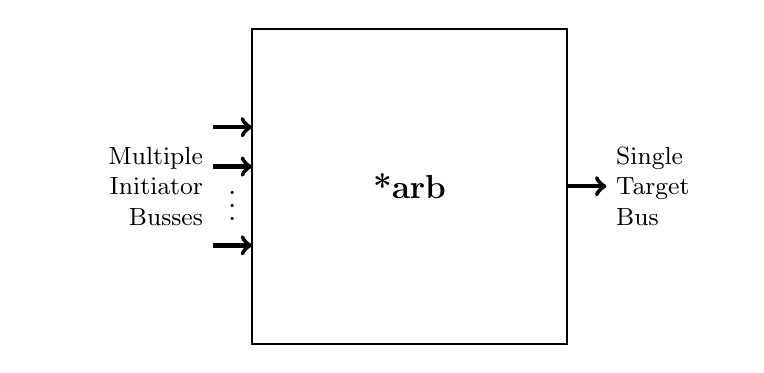
\begin{tikzpicture}
      %Block
      \draw [thick, fill=white] (4,0) rectangle (8,4);
      \node at (6,2)
            {\begin{minipage}[c]{8em}
                \begin{center}
                  \hyphenchar\font=-1
                  \large{\textbf{\nameref*{arb}}}
                \end{center}
             \end{minipage}};
      %Inputs     
      \node [left] at (3.5,2)
            {\begin{minipage}[c]{6em}
                \begin{flushright}
                  \hyphenchar\font=-1
                  \small{Multiple Initiator Busses}
                \end{flushright}
             \end{minipage}};
      \draw [ultra thick, ->] (3.5,2.75) -- (4,2.75);
      \draw [ultra thick, ->] (3.5,2.25) -- (4,2.25);
      \node [rotate=90] at (3.75,1.75) {\small{\texttt{...}}};
      \draw [ultra thick, ->] (3.5,1.25) -- (4,1.25);
     %Outputs     
      \node [right] at (8.5,2)
            {\begin{minipage}[c]{4em}
                \begin{flushleft}
                  \hyphenchar\font=-1
                  \small{Single Target Bus}
                \end{flushleft}
             \end{minipage}};
      \draw [ultra thick, ->] (8,2) -- (8.5,2);
    \end{tikzpicture}
    \caption{Block Diagram of the \nameref*{arb}}
    \label{arb:diag}
  \end{center}
\end{figure}
  
\subsubsection{Integration Parameters}
\label{arb:param}

The \nameref*{arb} supports the integration parameters listed in \tabref{arb:param:tab}. 
See \secref{param} for a detailed description of all integration parameters.

\begin{center}
  \rowcolors{1}{gray!12}{white}                                         %set alternating row color
  \begin{longtable}{|l|r|l|}
    \rowcolor{white}
    \caption{Integration Parameters of the \nameref*{arb}}
    \label{arb:param:tab} \\
    %Header
    \hline                                     
    \rowcolor{gray!25}
    \multicolumn{1}{|c|}{\textbf{\rule{0pt}{2.5ex} Parameter}}  &  
    \multicolumn{1}{c|}{\textbf{\rule{0pt}{2.5ex}  Default}}    & 
    \multicolumn{1}{c|}{\textbf{\rule{0pt}{2.5ex}  Decription}} \\
    \hline                                    
    \endhead                               
    %Footers
    \hline
    \rowcolor{white}
    \multicolumn{3}{r}{\tiny{...continued}} \\
    \endfoot
    \hline
    \endlastfoot
    %Content
    \texttt{ITR\_CNT   } & \texttt{4}  & Number of initiator busses           \\
    \texttt{ADR\_WIDTH} & \texttt{16}  & Width of the address bus             \\
    \texttt{DAT\_WIDTH} & \texttt{16}  & Width of each data bus               \\
    \texttt{SEL\_WIDTH } & \texttt{2}  & Number of data select lines          \\
    \texttt{TGA\_WIDTH } & \texttt{1}  & Number of address tags               \\
    \texttt{TGC\_WIDTH } & \texttt{1}  & Number of cycle tags                 \\
    \texttt{TGRD\_WIDTH} & \texttt{1}  & Number of read data tags             \\
    \texttt{TGWD\_WIDTH} & \texttt{1}  & Number of write data tags            \\
  \end{longtable}
\end{center}

\subsubsection{Interface Signals}
\label{arb:sig}

\tabref{arb:sig:tab} lists the interface signals of the \nameref*{arb}. 
See \secref{sig} for a detailed description of all interface signals.

\begingroup
\setlength{\LTleft}{-20cm plus -1fill}
\setlength{\LTright}{\LTleft}
\begin{center}
  \rowcolors{1}{gray!12}{white}                                         %set alternating row color
  \begin{longtable}{|l|r|l|l|}
    \rowcolor{white}
    \caption{Interface Signals of the \nameref*{arb}}
    \label{arb:sig:tab} \\
    %Header
    \hline                                     
    \rowcolor{gray!25}
    \multicolumn{1}{|c|}{\textbf{\rule{0pt}{2.5ex} Signal}}     &  
    \multicolumn{1}{c|}{\textbf{\rule{0pt}{2.5ex}  Range}}      & 
    \multicolumn{1}{c|}{\textbf{\rule{0pt}{2.5ex}  Direction}}  & 
    \multicolumn{1}{c|}{\textbf{\rule{0pt}{2.5ex}  Decription}} \\
    \hline
    \endhead                               
    %Footers
    \hline
    \rowcolor{white}
    \multicolumn{4}{r}{\tiny{...continued}} \\
    \endfoot
    \hline
    \endlastfoot
    %Section 'Clock and Reset'
    %\hline
    \rowcolor{gray!20}
    \multicolumn{4}{|c|}{\scriptsize{\rule{0pt}{2.5ex} Clock and Reset}} \global\rownum=1\relax \\  
    \hline                                    
    \texttt{clk\_i}        &                                & input & module clock              \\
    \texttt{async\_rst\_i} &                                & input & asynchronous reset        \\
    \texttt{sync\_rst\_i}  &                                & input & synchronous reset         \\
    %Section 'Initiator Interface'
    \hline                                 
    \rowcolor{gray!20}
    \multicolumn{4}{|c|}{\scriptsize{\rule{0pt}{2.5ex} Initiator Interface}} \global\rownum=1\relax \\    
    \hline                                 
    \texttt{itr\_cyc\_i}   & \texttt{ITR\_CNT-1:0}                 & input  & concatinated bus cycle indicators    \\
    \texttt{itr\_stb\_i}   & \texttt{ITR\_CNT-1:0}                 & input  & concatinated access requests	   \\
    \texttt{itr\_we\_i}    & \texttt{ITR\_CNT-1:0}                 & input  & concatinated write enables	   \\
    \texttt{itr\_lock\_i}  & \texttt{ITR\_CNT-1:0}                 & input  & concatinated bus cycle locks	   \\
    \texttt{itr\_sel\_i}   & \texttt{(ITR\_CNT*SEL\_WIDTH)-1:0}    & input  & concatinated write data selects	   \\
    \texttt{itr\_adr\_i}   & \texttt{(ITR\_CNT*ADR\_WIDTH)-1:0}   & input  & concatinated address busses	   \\
    \texttt{itr\_dat\_i}   & \texttt{(ITR\_CNT*DAT\_WIDTH)-1:0}   & input  & concatinated write data busses	   \\
    \texttt{itr\_tga\_i}   & \texttt{(ITR\_CNT*TGA\_WIDTH)-1:0}    & input  & concatinated address tags	           \\
    \texttt{itr\_tga\_prio\_i} & \texttt{ITR\_CNT-1:0}             & input  & concatinated access priorities	   \\
    \texttt{itr\_tgc\_i}   & \texttt{(ITR\_CNT*TGC\_WIDTH)-1:0}    & input  & concatinated bus cycle tags	   \\
    \texttt{itr\_tgd\_i}   & \texttt{(ITR\_CNT*TGWD\_WIDTH)-1:0}   & input  & concatinated write data tags	   \\
    \texttt{itr\_ack\_o}   & \texttt{ITR\_CNT-1:0}                 & output & concatinated bus cycle acknowledges  \\
    \texttt{itr\_err\_o}   & \texttt{ITR\_CNT-1:0}                 & output & concatinated error indicators	   \\
    \texttt{itr\_rty\_o}   & \texttt{ITR\_CNT-1:0}                 & output & concatinated retry requests	   \\
    \texttt{itr\_stall\_o} & \texttt{ITR\_CNT-1:0}                 & output & concatinated access delays	   \\
    \texttt{itr\_dat\_o}   & \texttt{(ITR\_CNT*DAT\_WIDTH)-1:0}   & output & concatinated read data buses	   \\
    \texttt{itr\_tgd\_o}   & \texttt{(ITR\_CNT*TGRD\_WIDTH)-1:0}   & output & concatinated read data tags          \\ 
    %Section 'Target Interface'
    \hline                                                                                      
    \rowcolor{gray!20}
    \multicolumn{4}{|c|}{\scriptsize{\rule{0pt}{2.5ex} Target Interface}} \global\rownum=1\relax \\  
    \hline                                                                                      
    \texttt{tgt\_cyc\_o}         &                          & output & bus cycle indicator       \\
    \texttt{tgt\_stb\_o}         &                          & output & access request            \\
    \texttt{tgt\_we\_o}          &                          & output & write enable              \\
    \texttt{tgt\_lock\_o}        &                          & output & uninterruptable bus cycle \\
    \texttt{tgt\_sel\_o}         & \texttt{SEL\_WIDTH-1:0}  & output & write data selects        \\
    \texttt{tgt\_adr\_o}         & \texttt{ADR\_WIDTH-1:0}  & output & write data selects        \\
    \texttt{tgt\_dat\_o}         & \texttt{DAT\_WIDTH-1:0}  & output & write data bus            \\
    \texttt{tgt\_tga\_o}         & \texttt{TGA\_WIDTH-1:0}  & output & address tags              \\
    \texttt{tgt\_tgc\_o}         & \texttt{TGC\_WIDTH-1:0}  & output & bus cycle tags            \\
    \texttt{tgt\_tgd\_o}         & \texttt{TGWD\_WIDTH-1:0} & output & write data tags           \\
    \texttt{tgt\_ack\_i}         &                          & input  & bus cycle acknowledge     \\
    \texttt{tgt\_err\_i}         &                          & input  & error indicator           \\
    \texttt{tgt\_rty\_i}         &                          & input  & retry request             \\
    \texttt{tgt\_stall\_i}       &                          & input  & access delay              \\
    \texttt{tgt\_dat\_i}         & \texttt{DAT\_WIDTH-1:0}  & input  & read data bus             \\
    \texttt{tgt\_tgd\_i}         & \texttt{TGRD\_WIDTH-1:0} & input  & read data tags            \\   
  \end{longtable}
\end{center}  
\endgroup

\subsubsection{Verification Status}
\label{arb:verif}

\tabref[Table]{arb:verif:tab} provides an overview of the verification status of the \nameref*{arb}.
Lint checks have been done with the Icarus Verilog simulator~\cite{iverilog} and the Yosys synthesis tool~\cite{yosys}.

\begin{center}
  \rowcolors{1}{gray!12}{white}                                         %set alternating row color
  \begin{longtable}{|lr|c|c|c|c|}
    \rowcolor{white}
    \caption[Interface Signals]{Verification Status of the \nameref*{arb}}
    \label{arb:verif:tab} \\
    %Header
    \hline                              
    \rowcolor{gray!25}
    \multicolumn{2}{|c|}{\textbf{\rule{0pt}{2.5ex} Configuration}} &  
    \multicolumn{1}{c|}{\textbf{\rule{0pt}{2.5ex}  Linting}}       &  
    \multicolumn{1}{c|}{\textbf{\rule{0pt}{2.5ex}  Simulation}}    &  
    \multicolumn{1}{c|}{\textbf{\rule{0pt}{2.5ex}  Formal}}        &  
    \multicolumn{1}{c|}{\textbf{\rule{0pt}{2.5ex}  FPGA}}          \\
    \hline                              
    \endhead                               
    %Footers
    \hline
    \rowcolor{white}
    \multicolumn{6}{r}{\tiny{...continued}} \\
    \endfoot
    \hline
    \endlastfoot
    %Content
    \makecell[l]{\underline{\smash{\texttt{default}:}} \\ 
                 \texttt{ITR\_CNT}    \\
                 \texttt{ADR\_WIDTH}  \\
                 \texttt{DAT\_WIDTH}  \\
                 \texttt{SEL\_WIDTH}  \\
                 \texttt{TGA\_WIDTH}  \\
                 \texttt{TGC\_WIDTH}  \\
                 \texttt{TGRD\_WIDTH} \\
                 \texttt{TGWD\_WIDTH}}   &
    \makecell[r]{                     \\ 
                 \texttt{4}           \\
                 \texttt{16}          \\
                 \texttt{16}          \\
                 \texttt{2}           \\
                 \texttt{1}           \\
                 \texttt{1}           \\
                 \texttt{1}           \\
                 \texttt{1}}             &     
    \makecell[c]{iVerilog~\cite{iverilog} \\                    
                 Yosis~\cite{yosys}}     &
    & & \\
  \end{longtable}
\end{center}
  


%###############################################################################
%# WbXbc - Manual - Bus Width Expander                                         #
%###############################################################################
%#    Copyright 2018 Dirk Heisswolf                                            #
%#    This file is part of the WbXbc project.                                  #
%#                                                                             #
%#    WbXbc is free software: you can redistribute it and/or modify            #
%#    it under the terms of the GNU General Public License as published by     #
%#    the Free Software Foundation, either version 3 of the License, or        #
%#    (at your option) any later version.                                      #
%#                                                                             #
%#    WbXbc is distributed in the hope that it will be useful,                 #
%#    but WITHOUT ANY WARRANTY; without even the implied warranty of           #
%#    MERCHANTABILITY or FITNESS FOR A PARTICULAR PURPOSE.  See the            #
%#    GNU General Public License for more details.                             #
%#                                                                             #
%#    You should have received a copy of the GNU General Public License        #
%#    along with WbXbc.  If not, see <http://www.gnu.org/licenses/>.           #
%###############################################################################
%# Version History:                                                            #
%#   September 27, 2018                                                        #
%#      - Initial release                                                      #
%###############################################################################

\subsection[WbXbc Address Decoder]{WbXbc Expander (\texttt{WbXbc\_expander})}
\label{expand}

This module connects a pipelined Wishbone initiator to a target with twice the
data bus width (see \figref{expand:diag}).
%               +-------------------+            
%               |                   |            
%               |                   |            
% Narrow        |      WbXbc        |     Wide  
% Initiator --->|      Expander     +---> Target 
% Bus           |                   |     Bus   
%               |                   |            
%               |                   |            
%               +-------------------+            
\begin{figure}[!h]
  \begin{center}
    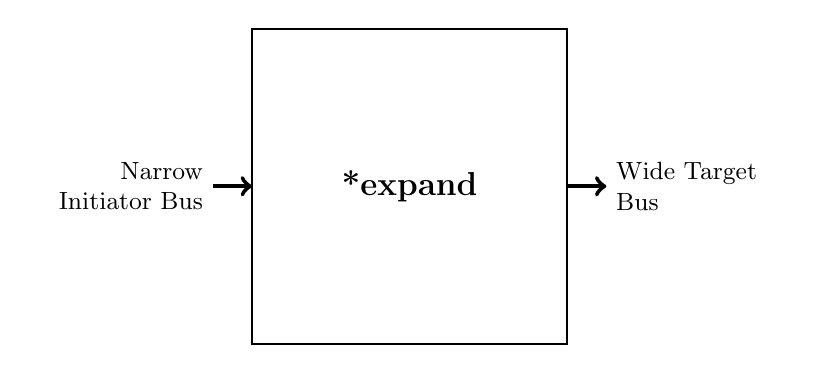
\begin{tikzpicture}
      %Block
      \draw [thick, fill=white] (4,0) rectangle (8,4);
      \node at (6,2)
            {\begin{minipage}[c]{8em}
                \begin{center}
                  \hyphenchar\font=-1
                  \large{\textbf{\nameref*{expand}}}
                \end{center}
             \end{minipage}};
      %Inputs     
      \node [left] at (3.5,2)
            {\begin{minipage}[c]{6em}
                \begin{flushright}
                  \hyphenchar\font=-1
                  \small{Narrow Initiator Bus}
                \end{flushright}
             \end{minipage}};
      \draw [ultra thick, ->] (3.5,2) -- (4,2);
      %Outputs     
      \node [right] at (8.5,2)
            {\begin{minipage}[c]{6em}
                \begin{flushleft}
                  \hyphenchar\font=-1
                  \small{Wide Target Bus}
                \end{flushleft}
             \end{minipage}};
      \draw [ultra thick, ->] (8,2) -- (8.5,2);
    \end{tikzpicture}
    \caption{Block Diagram of the \nameref*{expand}}
    \label{expand:diag}
  \end{center}
\end{figure}
  
\subsubsection{Integration Parameters}
\label{expand:param}

The \nameref*{expand} supports the integration parameters listed in \tabref{expand:param:tab}. 
See \secref{param} for a detailed description of all integration parameters.

\begin{center}
  \rowcolors{1}{gray!12}{white}                                         %set alternating row color
  \begin{longtable}{|l|r|l|}
    \rowcolor{white}
    \caption{Integration Parameters of the \nameref*{expand}}
    \label{expand:param:tab} \\
    %Header
    \hline                                     
    \rowcolor{gray!25}
    \multicolumn{1}{|c|}{\textbf{\rule{0pt}{2.5ex} Parameter}}  &  
    \multicolumn{1}{c|}{\textbf{\rule{0pt}{2.5ex}  Default}}    & 
    \multicolumn{1}{c|}{\textbf{\rule{0pt}{2.5ex}  Decription}} \\
    \hline                                    
    \endhead                               
    %Footers
    \hline
    \rowcolor{white}
    \multicolumn{3}{r}{\tiny{...continued}} \\
    \endfoot
    \hline
    \endlastfoot
    %Content
    \texttt{ITR\_ADDR\_WIDTH} & \texttt{16} & Width of the address bus             \\
    \texttt{ITR\_DATA\_WIDTH} & \texttt{16} & Width of each data bus               \\
    \texttt{ITR\_SEL\_WIDTH } & \texttt{2}  & Number of data select lines          \\
    \texttt{TGA\_WIDTH }      & \texttt{1}  & Number of address tags               \\
    \texttt{TGC\_WIDTH }      & \texttt{1}  & Number of cycle tags                 \\
    \texttt{TGRD\_WIDTH}      & \texttt{1}  & Number of read data tags             \\
    \texttt{TGWD\_WIDTH}      & \texttt{1}  & Number of write data tags            \\
    \texttt{BIG\_ENDIAN}      & \texttt{1}  & Endianess of the component           \\
  \end{longtable}
\end{center}

\subsubsection{Interface Signals}
\label{expand:sig}

\tabref{expand:sig:tab} lists the interface signals of the \nameref*{expand}. 
See \secref{sig} for a detailed description of all interface signals.

\begin{center}
  \rowcolors{1}{gray!12}{white}                                         %set alternating row color
  \begin{longtable}{|l|r|l|l|}
    \rowcolor{white}
    \caption{Interface Signals of the \nameref*{expand}}
    \label{expand:sig:tab} \\
    %Header
    \hline                                     
    \rowcolor{gray!25}
    \multicolumn{1}{|c|}{\textbf{\rule{0pt}{2.5ex} Signal}}     &  
    \multicolumn{1}{c|}{\textbf{\rule{0pt}{2.5ex}  Range}}      & 
    \multicolumn{1}{c|}{\textbf{\rule{0pt}{2.5ex}  Direction}}  & 
    \multicolumn{1}{c|}{\textbf{\rule{0pt}{2.5ex}  Decription}} \\
    \hline
    \endhead                               
    %Footers
    \hline
    \rowcolor{white}
    \multicolumn{4}{r}{\tiny{...continued}} \\
    \endfoot
    \hline
    \endlastfoot
    %Section 'Target Address Regions'
    %\hline
    \rowcolor{gray!20}
    \multicolumn{4}{|c|}{\scriptsize{\rule{0pt}{2.5ex} Target Address Regions}} \global\rownum=1\relax \\  
    \hline                                    
    \texttt{region\_addr\_i} & \texttt{(TGT\_CNT*ADDR\_WIDTH)\-1:0} & input & target address                             \\
    \texttt{region\_mask\_i} & \texttt{(TGT\_CNT*ADDR\_WIDTH)\-1:0} & input & \makecell[l]{selects relevant address bits \\
                                                                                           (1: relevant, 0: ignored)}    \\
    %Section 'Clock and Reset'
    %\hline
    \rowcolor{gray!20}
    \multicolumn{4}{|c|}{\scriptsize{\rule{0pt}{2.5ex} Clock and Reset}} \global\rownum=1\relax \\  
    \hline                                    
    \texttt{clk\_i}        &                                & input  & module clock              \\
    \texttt{async\_rst\_i} &                                & input  & asynchronous reset        \\
    \texttt{sync\_rst\_i}  &                                & input  & synchronous reset         \\
    %Section 'Initiator Interface'
    \hline                                 
    \rowcolor{gray!20}
    \multicolumn{4}{|c|}{\scriptsize{\rule{0pt}{2.5ex} Initiator Interface}} \global\rownum=1\relax \\    
    \hline                                 
    \texttt{itr\_cyc\_i}   &                                & input  & bus cycle indicator       \\
    \texttt{itr\_stb\_i}   &                                & input  & access request            \\
    \texttt{itr\_we\_i}    &                                & input  & write enable              \\
    \texttt{itr\_lock\_i}  &                                & input  & uninterruptable bus cycle \\
    \texttt{itr\_sel\_i}   & \texttt{ITR\_SEL\_WIDTH-1:0}   & input  & write data selects        \\
    \texttt{itr\_adr\_i}   & \texttt{ITR\_ADDR\_WIDTH-1:0}  & input  & address bus               \\
    \texttt{itr\_dat\_i}   & \texttt{ITR\_DATA\_WIDTH-1:0}  & input  & write data bus            \\
    \texttt{itr\_tga\_i}   & \texttt{TGA\_WIDTH-1:0}        & input  & address tags              \\
    \texttt{itr\_tgc\_i}   & \texttt{TGC\_WIDTH-1:0}        & input  & bus cycle tags            \\
    \texttt{itr\_tgd\_i}   & \texttt{TGWD\_WIDTH-1:0}       & input  & write data tags           \\
    \texttt{itr\_ack\_o}   &                                & output & bus cycle acknowledge     \\
    \texttt{itr\_err\_o}   &                                & output & error indicator           \\
    \texttt{itr\_rty\_o}   &                                & output & retry request             \\
    \texttt{itr\_stall\_o} &                                & output & access delay              \\
    \texttt{itr\_dat\_o}   & \texttt{DATA\_WIDTH-1:0}       & output & read data bus             \\
    \texttt{itr\_tgd\_o}   & \texttt{TGRD\_WIDTH-1:0}       & output & read data tags            \\ 
    %Section 'Target Interface'
    \hline                                                                                      
    \rowcolor{gray!20}
    \multicolumn{4}{|c|}{\scriptsize{\rule{0pt}{2.5ex} Target Interface}} \global\rownum=1\relax \\  
    \hline                                                                                      
    \texttt{tgt\_cyc\_o}         &                          & output & bus cycle indicator       \\
    \texttt{tgt\_stb\_o}         &                          & output & access request            \\
    \texttt{tgt\_we\_o}          &                          & output & write enable              \\
    \texttt{tgt\_lock\_o}        &                          & output & uninterruptable bus cycle \\
    \texttt{tgt\_sel\_o}         & \texttt{(ITR\_SEL\_WIDTH*2)-1:0}  & output & write data selects \\
    \texttt{tgt\_adr\_o}         & \texttt{ITR\_ADDR\_WIDTH-2:0}     & output & write data selects \\
    \texttt{tgt\_dat\_o}         & \texttt{(ITR\_DATA\_WIDTH*2)-1:0} & output & write data bus     \\
    \texttt{tgt\_tga\_o}         & \texttt{TGA\_WIDTH-1:0}  & output & address tags              \\
    \texttt{tgt\_tgc\_o}         & \texttt{TGC\_WIDTH-1:0}  & output & bus cycle tags            \\
    \texttt{tgt\_tgd\_o}         & \texttt{TGWD\_WIDTH-1:0} & output & write data tags           \\
    \texttt{tgt\_ack\_i}         &                          & input  & bus cycle acknowledge     \\
    \texttt{tgt\_err\_i}         &                          & input  & error indicator           \\
    \texttt{tgt\_rty\_i}         &                          & input  & retry request             \\
    \texttt{tgt\_stall\_i}       &                          & input  & access delay              \\
    \texttt{tgt\_dat\_i}         & \texttt{DATA\_WIDTH-1:0} & input  & read data bus             \\
    \texttt{tgt\_tgd\_i}         & \texttt{TGRD\_WIDTH-1:0} & input  & read data tags            \\   
  \end{longtable}
\end{center}  

\subsubsection{Verification Status}
\label{expand:verif}

\tabref[Table]{expand:verif:tab} provides an overview of the verification status of the \nameref*{expand}.
Lint checks have been done with the Icarus Verilog simulator~\cite{iverilog} and the Yosys synthesis tool~\cite{yosys}.

\begin{center}
  \rowcolors{1}{gray!12}{white}                                         %set alternating row color
  \begin{longtable}{|lr|c|c|c|c|}
    \rowcolor{white}
    \caption[Interface Signals]{Verification Status of the \nameref*{expand}}
    \label{expand:verif:tab} \\
    %Header
    \hline                              
    \rowcolor{gray!25}
    \multicolumn{2}{|c|}{\textbf{\rule{0pt}{2.5ex} Configuration}} &  
    \multicolumn{1}{c|}{\textbf{\rule{0pt}{2.5ex}  Linting}}       &  
    \multicolumn{1}{c|}{\textbf{\rule{0pt}{2.5ex}  Simulation}}    &  
    \multicolumn{1}{c|}{\textbf{\rule{0pt}{2.5ex}  Formal}}        &  
    \multicolumn{1}{c|}{\textbf{\rule{0pt}{2.5ex}  FPGA}}          \\
    \hline                              
    \endhead                               
    %Footers
    \hline
    \rowcolor{white}
    \multicolumn{6}{r}{\tiny{...continued}} \\
    \endfoot
    \hline
    \endlastfoot
    %Content
    \makecell[l]{Default:                   \\ 
                 \texttt{ITR\_ADDR\_WIDTH}  \\
                 \texttt{ITR\_DATA\_WIDTH}  \\
                 \texttt{ITR\_SEL\_WIDTH}   \\
                 \texttt{TGA\_WIDTH}        \\
                 \texttt{TGC\_WIDTH}        \\
                 \texttt{TGRD\_WIDTH}       \\
                 \texttt{TGWD\_WIDTH}       \\ 
                 \texttt{BIG\_ENDIAN}}   &  
    \makecell[r]{                           \\ 
                 \texttt{16}                \\
                 \texttt{16}                \\
                 \texttt{2}                 \\
                 \texttt{1}                 \\
                 \texttt{1}                 \\
                 \texttt{1}                 \\
                 \texttt{1}                 \\
                 \texttt{1}}             &      
    \makecell[c]{iVerilog~\cite{iverilog}   \\                    
                 Yosis~\cite{yosys}}     &
    & & \\
  \end{longtable}
\end{center}
  


%###############################################################################
%# WbXbc - Manual - Bus Width Reducer                                         #
%###############################################################################
%#    Copyright 2018 Dirk Heisswolf                                            #
%#    This file is part of the WbXbc project.                                  #
%#                                                                             #
%#    WbXbc is free software: you can redistribute it and/or modify            #
%#    it under the terms of the GNU General Public License as published by     #
%#    the Free Software Foundation, either version 3 of the License, or        #
%#    (at your option) any later version.                                      #
%#                                                                             #
%#    WbXbc is distributed in the hope that it will be useful,                 #
%#    but WITHOUT ANY WARRANTY; without even the implied warranty of           #
%#    MERCHANTABILITY or FITNESS FOR A PARTICULAR PURPOSE.  See the            #
%#    GNU General Public License for more details.                             #
%#                                                                             #
%#    You should have received a copy of the GNU General Public License        #
%#    along with WbXbc.  If not, see <http://www.gnu.org/licenses/>.           #
%###############################################################################
%# Version History:                                                            #
%#   September 27, 2018                                                        #
%#      - Initial release                                                      #
%###############################################################################

\subsection[WbXbc Reducer]{WbXbc Reducer (\texttt{WbXbc\_reducer})}
\label{reduc}

This module connects a pipelined Wishbone initiator to a target with    
half the data bus width (see \figref{reduc:diag}).   
Initiator bus accesses may be converted into two consecutive accesses to
the target bus.                                                         
%               +-------------------+            
%               |                   |            
%               |                   |            
% Wide          |      WbXbc        |     Narrow  
% Initiator --->|      Reducer      +---> Target 
% Bus           |                   |     Bus   
%               |                   |            
%               |                   |            
%               +-------------------+            
\begin{figure}[!h]
  \begin{center}
    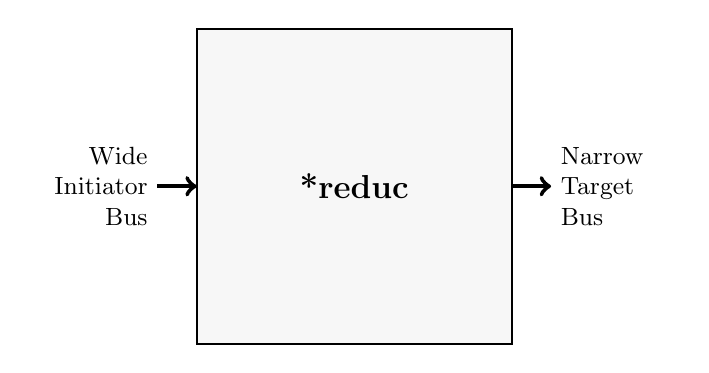
\begin{tikzpicture}
      %Block
      \draw [thick, fill=gray!6] (4,0) rectangle (8,4);
      \node at (6,2)
            {\begin{minipage}[c]{8em}
                \begin{center}
                  \hyphenchar\font=-1
                  \large{\textbf{\nameref*{reduc}}}
                \end{center}
             \end{minipage}};
      %Inputs     
      \node [left] at (3.5,2)
            {\begin{minipage}[c]{4em}
                \begin{flushright}
                  \hyphenchar\font=-1
                  \small{Wide Initiator Bus}
                \end{flushright}
             \end{minipage}};
      \draw [ultra thick, ->] (3.5,2) -- (4,2);
      %Outputs     
      \node [right] at (8.5,2)
            {\begin{minipage}[c]{4em}
                \begin{flushleft}
                  \hyphenchar\font=-1
                  \small{Narrow Target Bus}
                \end{flushleft}
             \end{minipage}};
      \draw [ultra thick, ->] (8,2) -- (8.5,2);
    \end{tikzpicture}
    \caption{Block Diagram of the \nameref*{reduc}}
    \label{reduc:diag}
  \end{center}
\end{figure}
  
\subsubsection{Integration Parameters}
\label{reduc:param}

The \nameref*{reduc} supports the integration parameters listed in \tabref{reduc:param:tab}. 
See \secref{param} for a detailed description of all integration parameters.

\begin{center}
  \rowcolors{1}{gray!12}{white}                                         %set alternating row color
  \begin{longtable}{|l|r|l|}
    \rowcolor{white}
    \caption{Integration Parameters of the \nameref*{reduc}}
    \label{reduc:param:tab} \\
    %Header
    \hline                                     
    \rowcolor{gray!25}
    \multicolumn{1}{|c|}{\textbf{\rule{0pt}{2.5ex} Parameter}}  &  
    \multicolumn{1}{c|}{\textbf{\rule{0pt}{2.5ex}  Default}}    & 
    \multicolumn{1}{c|}{\textbf{\rule{0pt}{2.5ex}  Decription}} \\
    \hline                                    
    \endhead                               
    %Footers
    \hline
    \rowcolor{white}
    \multicolumn{3}{r}{\tiny{...continued}} \\
    \endfoot
    \hline
    \endlastfoot
    %Content
    \texttt{ITR\_ADR\_WIDTH}  & \texttt{16} & Width of the address bus             \\
    \texttt{ITR\_DAT\_WIDTH}  & \texttt{16} & Width of each data bus               \\
    \texttt{ITR\_SEL\_WIDTH } & \texttt{2}  & Number of data select lines          \\
    \texttt{TGA\_WIDTH }      & \texttt{1}  & Number of address tags               \\
    \texttt{TGC\_WIDTH }      & \texttt{1}  & Number of cycle tags                 \\
    \texttt{TGRD\_WIDTH}      & \texttt{1}  & Number of read data tags             \\
    \texttt{TGWD\_WIDTH}      & \texttt{1}  & Number of write data tags            \\
    \texttt{BIG\_ENDIAN}      & \texttt{1}  & Endianess of the component           \\
  \end{longtable}
\end{center}

\subsubsection{Interface Signals}
\label{reduc:sig}

\tabref{reduc:sig:tab} lists the interface signals of the \nameref*{reduc}. 
See \secref{sig} for a detailed description of all interface signals.

\begin{center}
  \rowcolors{1}{gray!12}{white}                                         %set alternating row color
  \begin{longtable}{|l|r|l|l|}
    \rowcolor{white}
    \caption{Interface Signals of the \nameref*{reduc}}
    \label{reduc:sig:tab} \\
    %Header
    \hline                                     
    \rowcolor{gray!25}
    \multicolumn{1}{|c|}{\textbf{\rule{0pt}{2.5ex} Signal}}     &  
    \multicolumn{1}{c|}{\textbf{\rule{0pt}{2.5ex}  Range}}      & 
    \multicolumn{1}{c|}{\textbf{\rule{0pt}{2.5ex}  Direction}}  & 
    \multicolumn{1}{c|}{\textbf{\rule{0pt}{2.5ex}  Decription}} \\
    \hline
    \endhead                               
    %Footers
    \hline
    \rowcolor{white}
    \multicolumn{4}{r}{\tiny{...continued}} \\
    \endfoot
    \hline
    \endlastfoot
    %Section 'Target Address Regions'
    %\hline
    \rowcolor{gray!20}
    \multicolumn{4}{|c|}{\scriptsize{\rule{0pt}{2.5ex} Target Address Regions}} \global\rownum=1\relax \\  
    \hline                                    
    \texttt{region\_addr\_i} & \texttt{(TGT\_CNT*ADR\_WIDTH)\-1:0} & input & target address                             \\
    \texttt{region\_mask\_i} & \texttt{(TGT\_CNT*ADR\_WIDTH)\-1:0} & input & \makecell[l]{selects relevant address bits \\
                                                                                           (1: relevant, 0: ignored)}    \\
    %Section 'Clock and Reset'
    %\hline
    \rowcolor{gray!20}
    \multicolumn{4}{|c|}{\scriptsize{\rule{0pt}{2.5ex} Clock and Reset}} \global\rownum=1\relax \\  
    \hline                                    
    \texttt{clk\_i}        &                                & input & module clock              \\
    \texttt{async\_rst\_i} &                                & input & asynchronous reset        \\
    \texttt{sync\_rst\_i}  &                                & input & synchronous reset         \\
    %Section 'Initiator Interface'
    \hline                                 
    \rowcolor{gray!20}
    \multicolumn{4}{|c|}{\scriptsize{\rule{0pt}{2.5ex} Initiator Interface}} \global\rownum=1\relax \\    
    \hline                                 
    \texttt{itr\_cyc\_i}   &                                & input  & bus cycle indicator       \\
    \texttt{itr\_stb\_i}   &                                & input  & access request            \\
    \texttt{itr\_we\_i}    &                                & input  & write enable              \\
    \texttt{itr\_lock\_i}  &                                & input  & uninterruptable bus cycle \\
    \texttt{itr\_sel\_i}   & \texttt{ITR\_SEL\_WIDTH-1:0}   & input  & write data selects        \\
    \texttt{itr\_adr\_i}   & \texttt{ITR\_ADR\_WIDTH-1:0}   & input  & address bus               \\
    \texttt{itr\_dat\_i}   & \texttt{ITR\_DAT\_WIDTH-1:0}   & input  & write data bus            \\
    \texttt{itr\_tga\_i}   & \texttt{TGA\_WIDTH-1:0}        & input  & address tags              \\
    \texttt{itr\_tgc\_i}   & \texttt{TGC\_WIDTH-1:0}        & input  & bus cycle tags            \\
    \texttt{itr\_tgd\_i}   & \texttt{TGWD\_WIDTH-1:0}       & input  & write data tags           \\
    \texttt{itr\_ack\_o}   &                                & output & bus cycle acknowledge     \\
    \texttt{itr\_err\_o}   &                                & output & error indicator           \\
    \texttt{itr\_rty\_o}   &                                & output & retry request             \\
    \texttt{itr\_stall\_o} &                                & output & access delay              \\
    \texttt{itr\_dat\_o}   & \texttt{DAT\_WIDTH-1:0}        & output & read data bus             \\
    \texttt{itr\_tgd\_o}   & \texttt{TGRD\_WIDTH-1:0}       & output & read data tags            \\ 
    %Section 'Target Interface'
    \hline                                                                                      
    \rowcolor{gray!20}
    \multicolumn{4}{|c|}{\scriptsize{\rule{0pt}{2.5ex} Target Interface}} \global\rownum=1\relax \\  
    \hline                                                                                      
    \texttt{tgt\_cyc\_o}         &                          & output & bus cycle indicator       \\
    \texttt{tgt\_stb\_o}         &                          & output & access request            \\
    \texttt{tgt\_we\_o}          &                          & output & write enable              \\
    \texttt{tgt\_lock\_o}        &                          & output & uninterruptable bus cycle \\
    \texttt{tgt\_sel\_o}         & \texttt{(ITR\_SEL\_WIDTH/2)-1:0}  & output & write data selects \\
    \texttt{tgt\_adr\_o}         & \texttt{ITR\_ADR\_WIDTH:0}        & output & write data selects \\
    \texttt{tgt\_dat\_o}         & \texttt{(ITR\_DAT\_WIDTH/2)-1:0}  & output & write data bus     \\
    \texttt{tgt\_tga\_o}         & \texttt{TGA\_WIDTH-1:0}  & output & address tags              \\
    \texttt{tgt\_tgc\_o}         & \texttt{TGC\_WIDTH-1:0}  & output & bus cycle tags            \\
    \texttt{tgt\_tgd\_o}         & \texttt{TGWD\_WIDTH-1:0} & output & write data tags           \\
    \texttt{tgt\_ack\_i}         &                          & input  & bus cycle acknowledge     \\
    \texttt{tgt\_err\_i}         &                          & input  & error indicator           \\
    \texttt{tgt\_rty\_i}         &                          & input  & retry request             \\
    \texttt{tgt\_stall\_i}       &                          & input  & access delay              \\
    \texttt{tgt\_dat\_i}         & \texttt{DAT\_WIDTH-1:0} & input   & read data bus             \\
    \texttt{tgt\_tgd\_i}         & \texttt{TGRD\_WIDTH-1:0} & input  & read data tags            \\   
  \end{longtable}
\end{center}  

\subsubsection{Verification Status}
\label{reduc:verif}

\tabref[Table]{reduc:verif:tab} provides an overview of the verification status of the \nameref*{reduc}.
Lint checks have been done with the Icarus Verilog simulator~\cite{iverilog} and the Yosys synthesis tool~\cite{yosys}.

\begin{center}
  \rowcolors{1}{gray!12}{white}                                         %set alternating row color
  \begin{longtable}{|lr|c|c|c|c|}
    \rowcolor{white}
    \caption[Interface Signals]{Verification Status of the \nameref*{reduc}}
    \label{reduc:verif:tab} \\
    %Header
    \hline                              
    \rowcolor{gray!25}
    \multicolumn{2}{|c|}{\textbf{\rule{0pt}{2.5ex} Configuration}} &  
    \multicolumn{1}{c|}{\textbf{\rule{0pt}{2.5ex}  Linting}}       &  
    \multicolumn{1}{c|}{\textbf{\rule{0pt}{2.5ex}  Simulation}}    &  
    \multicolumn{1}{c|}{\textbf{\rule{0pt}{2.5ex}  Formal}}        &  
    \multicolumn{1}{c|}{\textbf{\rule{0pt}{2.5ex}  FPGA}}          \\
    \hline                              
    \endhead                               
    %Footers
    \hline
    \rowcolor{white}
    \multicolumn{6}{r}{\tiny{...continued}} \\
    \endfoot
    \hline
    \endlastfoot
    %Content
    \makecell[l]{\underline{\smash{\texttt{default}:}} \\ 
                 \texttt{ITR\_ADR\_WIDTH}   \\
                 \texttt{ITR\_DAT\_WIDTH}   \\
                 \texttt{ITR\_SEL\_WIDTH}   \\
                 \texttt{TGA\_WIDTH}        \\
                 \texttt{TGC\_WIDTH}        \\
                 \texttt{TGRD\_WIDTH}       \\
                 \texttt{TGWD\_WIDTH}       \\  
                 \texttt{BIG\_ENDIAN}}   &  
    \makecell[r]{                           \\ 
                 \texttt{16}                \\
                 \texttt{16}                \\
                 \texttt{2}                 \\
                 \texttt{1}                 \\
                 \texttt{1}                 \\
                 \texttt{1}                 \\
                 \texttt{1}                 \\
                 \texttt{1}}             &      
    \makecell[c]{iVerilog~\cite{iverilog}   \\                    
                 Yosis~\cite{yosys}}     &
    & & \\
    \hline
    \makecell[l]{\underline{\smash{\texttt{little\_endian}:}} \\ 
                 \texttt{ITR\_ADR\_WIDTH}   \\
                 \texttt{ITR\_DAT\_WIDTH}   \\
                 \texttt{ITR\_SEL\_WIDTH}   \\
                 \texttt{TGA\_WIDTH}        \\
                 \texttt{TGC\_WIDTH}        \\
                 \texttt{TGRD\_WIDTH}       \\
                 \texttt{TGWD\_WIDTH}       \\  
                 \texttt{BIG\_ENDIAN}}   &  
    \makecell[r]{                           \\ 
                 \texttt{16}                \\
                 \texttt{16}                \\
                 \texttt{2}                 \\
                 \texttt{1}                 \\
                 \texttt{1}                 \\
                 \texttt{1}                 \\
                 \texttt{1}                 \\
                 \texttt{0}}             &      
    \makecell[c]{iVerilog~\cite{iverilog}   \\                    
                 Yosis~\cite{yosys}}     &
    & & \\
  \end{longtable}
\end{center}
  


%###############################################################################
%# WbXbc - Manual - Slow to Fast Bus Gasket                                    #
%###############################################################################
%#    Copyright 2018 Dirk Heisswolf                                            #
%#    This file is part of the WbXbc project.                                  #
%#                                                                             #
%#    WbXbc is free software: you can redistribute it and/or modify            #
%#    it under the terms of the GNU General Public License as published by     #
%#    the Free Software Foundation, either version 3 of the License, or        #
%#    (at your option) any later version.                                      #
%#                                                                             #
%#    WbXbc is distributed in the hope that it will be useful,                 #
%#    but WITHOUT ANY WARRANTY; without even the implied warranty of           #
%#    MERCHANTABILITY or FITNESS FOR A PARTICULAR PURPOSE.  See the            #
%#    GNU General Public License for more details.                             #
%#                                                                             #
%#    You should have received a copy of the GNU General Public License        #
%#    along with WbXbc.  If not, see <http://www.gnu.org/licenses/>.           #
%###############################################################################
%# Version History:                                                            #
%#   October 1, 2018                                                           #
%#      - Initial release                                                      #
%###############################################################################

\subsection[WbXbc Accelerator]{WbXbc Accelerator (\texttt{WbXbc\_accelerator})}
\label{accel}

This module connects a pipelined Wishbone initiator, running at a higher
frequency to a target, running at a lower frequency (see \figref{accel:diag}).                    
%               +-------------------+           
%               |                   |           
%               |                   |           
% Slow          |    WbXbc          |     Fast  
% Initiator --->|    Accelerator    +---> Target
% Bus           |                   |     Bus  
%               |                   |           
%               |                   |           
%               +-------------------+           
\begin{figure}[!h]
  \begin{center}
    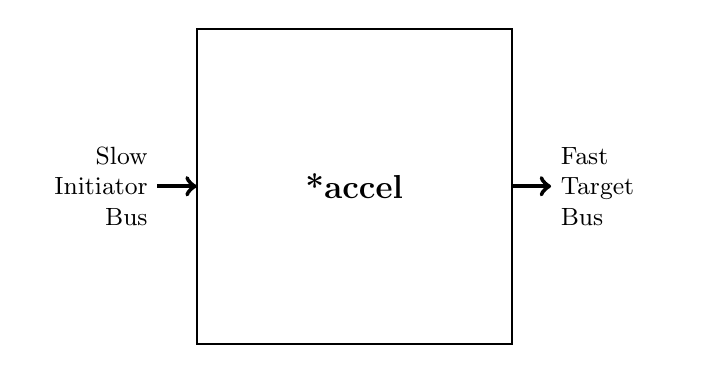
\begin{tikzpicture}
      %Block
      \draw [thick, fill=white] (4,0) rectangle (8,4);
      \node at (6,2)
            {\begin{minipage}[c]{8em}
                \begin{center}
                  \hyphenchar\font=-1
                  \large{\textbf{\nameref*{accel}}}
                \end{center}
             \end{minipage}};
      %Inputs     
      \node [left] at (3.5,2)
            {\begin{minipage}[c]{4em}
                \begin{flushright}
                  \hyphenchar\font=-1
                  \small{Slow Initiator Bus}
                \end{flushright}
             \end{minipage}};
      \draw [ultra thick, ->] (3.5,2) -- (4,2);
      %Outputs     
      \node [right] at (8.5,2)
            {\begin{minipage}[c]{4em}
                \begin{flushleft}
                  \hyphenchar\font=-1
                  \small{Fast Target Bus}
                \end{flushleft}
             \end{minipage}};
      \draw [ultra thick, ->] (8,2) -- (8.5,2);
    \end{tikzpicture}
    \caption{Block Diagram of the \nameref*{accel}}
    \label{accel:diag}
  \end{center}
\end{figure}
  
\subsubsection{Integration Parameters}
\label{accel:param}

The \nameref*{accel} supports the integration parameters listed in \tabref{accel:param:tab}. 
See \secref{param} for a detailed description of all integration parameters.

\begin{center}
  \rowcolors{1}{gray!12}{white}                                         %set alternating row color
  \begin{longtable}{|l|r|l|}
    \rowcolor{white}
    \caption{Integration Parameters of the \nameref*{accel}}
    \label{accel:param:tab} \\
    %Header
    \hline                                     
    \rowcolor{gray!25}
    \multicolumn{1}{|c|}{\textbf{\rule{0pt}{2.5ex} Parameter}}  &  
    \multicolumn{1}{c|}{\textbf{\rule{0pt}{2.5ex}  Default}}    & 
    \multicolumn{1}{c|}{\textbf{\rule{0pt}{2.5ex}  Decription}} \\
    \hline                                    
    \endhead                               
    %Footers
    \hline
    \rowcolor{white}
    \multicolumn{3}{r}{\tiny{...continued}} \\
    \endfoot
    \hline
    \endlastfoot
    %Content
    \texttt{ADR\_WIDTH}       & \texttt{16} & Width of the address bus             \\
    \texttt{DAT\_WIDTH}       & \texttt{16} & Width of each data bus               \\
    \texttt{SEL\_WIDTH }      & \texttt{2}  & Number of data select lines          \\
    \texttt{TGA\_WIDTH }      & \texttt{1}  & Number of address tags               \\
    \texttt{TGC\_WIDTH }      & \texttt{1}  & Number of cycle tags                 \\
    \texttt{TGRD\_WIDTH}      & \texttt{1}  & Number of read data tags             \\
    \texttt{TGWD\_WIDTH}      & \texttt{1}  & Number of write data tags            \\
    \texttt{REG\_ITR}         & \texttt{0}  & Register initiator bus inputs        \\
  \end{longtable}
\end{center}

\subsubsection{Interface Signals}
\label{accel:sig}

\tabref{accel:sig:tab} lists the interface signals of the \nameref*{accel}. 
See \secref{sig} for a detailed description of all interface signals.

\begingroup
\setlength{\LTleft}{-20cm plus -1fill}
\setlength{\LTright}{\LTleft}
\begin{center}
  \rowcolors{1}{gray!12}{white}                                         %set alternating row color
  \begin{longtable}{|l|r|l|l|}
    \rowcolor{white}
    \caption{Interface Signals of the \nameref*{accel}}
    \label{accel:sig:tab} \\
    %Header
    \hline                                     
    \rowcolor{gray!25}
    \multicolumn{1}{|c|}{\textbf{\rule{0pt}{2.5ex} Signal}}     &  
    \multicolumn{1}{c|}{\textbf{\rule{0pt}{2.5ex}  Range}}      & 
    \multicolumn{1}{c|}{\textbf{\rule{0pt}{2.5ex}  Direction}}  & 
    \multicolumn{1}{c|}{\textbf{\rule{0pt}{2.5ex}  Decription}} \\
    \hline
    \endhead                               
    %Footers
    \hline
    \rowcolor{white}
    \multicolumn{4}{r}{\tiny{...continued}} \\
    \endfoot
    \hline
    \endlastfoot
     %Section 'Clock and Reset'
    %\hline
    \rowcolor{gray!20}
    \multicolumn{4}{|c|}{\scriptsize{\rule{0pt}{2.5ex} Clock and Reset}} \global\rownum=1\relax \\*  
    \nobreakhline                                    
    \texttt{tgt\_clk\_i}   &                                & input & target clock              \\*
    \texttt{tgt2itr\_sync\_i} &                             & input & clock sync signal         \\*
    \texttt{async\_rst\_i} &                                & input & asynchronous reset        \\*
    \texttt{sync\_rst\_i}  &                                & input & synchronous reset         \\
    %Section 'Initiator Interface'
    \hline                                 
    \rowcolor{gray!20}
    \multicolumn{4}{|c|}{\scriptsize{\rule{0pt}{2.5ex} Initiator Interface}} \global\rownum=1\relax \\*    
    \hline                                 
    \texttt{itr\_cyc\_i}   &                                & input  & bus cycle indicator          \\*
    \texttt{itr\_stb\_i}   &                                & input  & access request               \\*
    \texttt{itr\_we\_i}    &                                & input  & write enable                 \\*
    \texttt{itr\_lock\_i}  &                                & input  & uninterruptable bus cycle    \\*
    \texttt{itr\_sel\_i}   & \texttt{SEL\_WIDTH-1:0}        & input  & write data selects           \\*
    \texttt{itr\_adr\_i}   & \texttt{ADR\_WIDTH-1:0}        & input  & address bus                  \\*
    \texttt{itr\_dat\_i}   & \texttt{DAT\_WIDTH-1:0}        & input  & write data bus               \\*
    \texttt{itr\_tga\_i}   & \texttt{TGA\_WIDTH-1:0}        & input  & address tags                 \\*
    \texttt{itr\_tgc\_i}   & \texttt{TGC\_WIDTH-1:0}        & input  & bus cycle tags               \\*
    \texttt{itr\_tgd\_i}   & \texttt{TGWD\_WIDTH-1:0}       & input  & write data tags              \\*
    \texttt{itr\_ack\_o}   &                                & output & bus cycle acknowledge        \\*
    \texttt{itr\_err\_o}   &                                & output & error indicator              \\*
    \texttt{itr\_rty\_o}   &                                & output & retry request                \\*
    \texttt{itr\_stall\_o} &                                & output & access delay                 \\*
    \texttt{itr\_dat\_o}   & \texttt{DAT\_WIDTH-1:0}        & output & read data bus                \\*
    \texttt{itr\_tgd\_o}   & \texttt{TGRD\_WIDTH-1:0}       & output & read data tags               \\ 
    %Section 'Target Interface'
    \hline                                                                                      
    \rowcolor{gray!20}
    \multicolumn{4}{|c|}{\scriptsize{\rule{0pt}{2.5ex} Target Interface}} \global\rownum=1\relax \\*  
    \nobreakhline                                                                                      
    \texttt{tgt\_cyc\_o}         &                          & output & bus cycle indicator       \\*
    \texttt{tgt\_stb\_o}         &                          & output & access request            \\*
    \texttt{tgt\_we\_o}          &                          & output & write enable              \\*
    \texttt{tgt\_lock\_o}        &                          & output & uninterruptable bus cycle \\*
    \texttt{tgt\_sel\_o}         & \texttt{SEL\_WIDTH-1:0}  & output & write data selects        \\*
    \texttt{tgt\_adr\_o}         & \texttt{ADR\_WIDTH-1:0}  & output & write data selects        \\*
    \texttt{tgt\_dat\_o}         & \texttt{DAT\_WIDTH-1:0}  & output & write data bus            \\*
    \texttt{tgt\_tga\_o}         & \texttt{TGA\_WIDTH-1:0}  & output & address tags              \\*
    \texttt{tgt\_tgc\_o}         & \texttt{TGC\_WIDTH-1:0}  & output & bus cycle tags            \\*
    \texttt{tgt\_tgd\_o}         & \texttt{TGWD\_WIDTH-1:0} & output & write data tags           \\*
    \texttt{tgt\_ack\_i}         &                          & input  & bus cycle acknowledge     \\*
    \texttt{tgt\_err\_i}         &                          & input  & error indicator           \\*
    \texttt{tgt\_rty\_i}         &                          & input  & retry request             \\*
    \texttt{tgt\_stall\_i}       &                          & input  & access delay              \\*
    \texttt{tgt\_dat\_i}         & \texttt{DAT\_WIDTH-1:0}  & input  & read data bus             \\*
    \texttt{tgt\_tgd\_i}         & \texttt{TGRD\_WIDTH-1:0} & input  & read data tags            \\   
  \end{longtable}
\end{center}  
\endgroup

\subsubsection{Verification Status}
\label{accel:verif}

\tabref[Table]{accel:verif:tab} provides an overview of the verification status of the \nameref*{accel}.
Lint checks have been done with the Icarus Verilog simulator~\cite{iverilog} and the Yosys synthesis tool~\cite{yosys}.

\begin{center}
  \rowcolors{1}{gray!12}{white}                                         %set alternating row color
  \begin{longtable}{|lr|c|c|c|c|}
    \rowcolor{white}
    \caption[Interface Signals]{Verification Status of the \nameref*{accel}}
    \label{accel:verif:tab} \\
    %Header
    \hline                              
    \rowcolor{gray!25}
    \multicolumn{2}{|c|}{\textbf{\rule{0pt}{2.5ex} Configuration}} &  
    \multicolumn{1}{c|}{\textbf{\rule{0pt}{2.5ex}  Linting}}       &  
    \multicolumn{1}{c|}{\textbf{\rule{0pt}{2.5ex}  Simulation}}    &  
    \multicolumn{1}{c|}{\textbf{\rule{0pt}{2.5ex}  Formal}}        &  
    \multicolumn{1}{c|}{\textbf{\rule{0pt}{2.5ex}  FPGA}}          \\
    \hline                              
    \endhead                               
    %Footers
    \hline
    \rowcolor{white}
    \multicolumn{6}{r}{\tiny{...continued}} \\
    \endfoot
    \hline
    \endlastfoot
    %Content
    \makecell[l]{Default:                   \\ 
                 \texttt{ADR\_WIDTH}        \\
                 \texttt{DAT\_WIDTH}        \\
                 \texttt{SEL\_WIDTH}        \\
                 \texttt{TGA\_WIDTH}        \\
                 \texttt{TGC\_WIDTH}        \\
                 \texttt{TGRD\_WIDTH}       \\
                 \texttt{TGWD\_WIDTH}       \\ 
                 \texttt{REG\_ITR}}   &  
    \makecell[r]{                           \\ 
                 \texttt{16}                \\
                 \texttt{16}                \\
                 \texttt{2}                 \\
                 \texttt{1}                 \\
                 \texttt{1}                 \\
                 \texttt{1}                 \\
                 \texttt{1}                 \\
                 \texttt{0}}             &      
    \makecell[c]{iVerilog~\cite{iverilog}   \\                    
                 Yosis~\cite{yosys}}     &
    & & \\
  \end{longtable}
\end{center}
  


%###############################################################################
%# WbXbc - Manual - Fast to Slow Bus Gasket                                    #
%###############################################################################
%#    Copyright 2018 Dirk Heisswolf                                            #
%#    This file is part of the WbXbc project.                                  #
%#                                                                             #
%#    WbXbc is free software: you can redistribute it and/or modify            #
%#    it under the terms of the GNU General Public License as published by     #
%#    the Free Software Foundation, either version 3 of the License, or        #
%#    (at your option) any later version.                                      #
%#                                                                             #
%#    WbXbc is distributed in the hope that it will be useful,                 #
%#    but WITHOUT ANY WARRANTY; without even the implied warranty of           #
%#    MERCHANTABILITY or FITNESS FOR A PARTICULAR PURPOSE.  See the            #
%#    GNU General Public License for more details.                             #
%#                                                                             #
%#    You should have received a copy of the GNU General Public License        #
%#    along with WbXbc.  If not, see <http://www.gnu.org/licenses/>.           #
%###############################################################################
%# Version History:                                                            #
%#   October 1, 2018                                                           #
%#      - Initial release                                                      #
%###############################################################################

\subsection[WbXbc Decelerator]{WbXbc Decelerator (\texttt{WbXbc\_decelerator})}
\label{decel}

This module connects a pipelined Wishbone initiator, running at a higher
frequency to a target, running at a lower frequency (see \figref{decel:diag}).                   
%               +-------------------+            
%               |                   |            
%               |                   |            
% Fast          |    WbXbc          |     Slow   
% Initiator --->|    Decelerator    +---> Target 
% Bus           |                   |     Bus   
%               |                   |            
%               |                   |            
%               +-------------------+            
\begin{figure}[!h]
  \begin{center}
    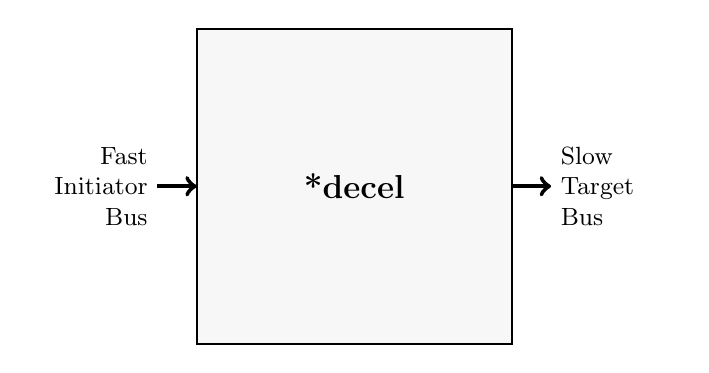
\begin{tikzpicture}
      %Block
      \draw [thick, fill=gray!6] (4,0) rectangle (8,4);
      \node at (6,2)
            {\begin{minipage}[c]{8em}
                \begin{center}
                  \hyphenchar\font=-1
                  \large{\textbf{\nameref*{decel}}}
                \end{center}
             \end{minipage}};
      %Inputs     
      \node [left] at (3.5,2)
            {\begin{minipage}[c]{4em}
                \begin{flushright}
                  \hyphenchar\font=-1
                  \small{Fast Initiator Bus}
                \end{flushright}
             \end{minipage}};
      \draw [ultra thick, ->] (3.5,2) -- (4,2);
      %Outputs     
      \node [right] at (8.5,2)
            {\begin{minipage}[c]{4em}
                \begin{flushleft}
                  \hyphenchar\font=-1
                  \small{Slow Target Bus}
                \end{flushleft}
             \end{minipage}};
      \draw [ultra thick, ->] (8,2) -- (8.5,2);
    \end{tikzpicture}
    \caption{Block Diagram of the \nameref*{decel}}
    \label{decel:diag}
  \end{center}
\end{figure}
  
\subsubsection{Integration Parameters}
\label{decel:param}

The \nameref*{decel} supports the integration parameters listed in \tabref{decel:param:tab}. 
See \secref{param} for a detailed description of all integration parameters.

\begin{center}
  \rowcolors{1}{gray!12}{white}                                         %set alternating row color
  \begin{longtable}{|l|r|l|}
    \rowcolor{white}
    \caption{Integration Parameters of the \nameref*{decel}}
    \label{decel:param:tab} \\
    %Header
    \hline                                     
    \rowcolor{gray!25}
    \multicolumn{1}{|c|}{\textbf{\rule{0pt}{2.5ex} Parameter}}  &  
    \multicolumn{1}{c|}{\textbf{\rule{0pt}{2.5ex}  Default}}    & 
    \multicolumn{1}{c|}{\textbf{\rule{0pt}{2.5ex}  Decription}} \\
    \hline                                    
    \endhead                               
    %Footers
    \hline
    \rowcolor{white}
    \multicolumn{3}{r}{\tiny{...continued}} \\
    \endfoot
    \hline
    \endlastfoot
    %Content
    \texttt{ADR\_WIDTH}       & \texttt{16} & Width of the address bus             \\
    \texttt{DAT\_WIDTH}       & \texttt{16} & Width of each data bus               \\
    \texttt{SEL\_WIDTH }      & \texttt{2}  & Number of data select lines          \\
    \texttt{TGA\_WIDTH }      & \texttt{1}  & Number of address tags               \\
    \texttt{TGC\_WIDTH }      & \texttt{1}  & Number of cycle tags                 \\
    \texttt{TGRD\_WIDTH}      & \texttt{1}  & Number of read data tags             \\
    \texttt{TGWD\_WIDTH}      & \texttt{1}  & Number of write data tags            \\
    \texttt{REG\_ITR}         & \texttt{0}  & Register initiator bus inputs        \\
    \texttt{REG\_TGT}         & \texttt{0}  & Register target bus inputs           \\
  \end{longtable}
\end{center}

\pagebreak

\subsubsection{Interface Signals}
\label{decel:sig}

\tabref{decel:sig:tab} lists the interface signals of the \nameref*{decel}. 
See \secref{sig} for a detailed description of all interface signals.

\begin{center}
  \rowcolors{1}{gray!12}{white}                                         %set alternating row color
  \begin{longtable}{|l|r|l|l|}
    \rowcolor{white}
    \caption{Interface Signals of the \nameref*{decel}}
    \label{decel:sig:tab} \\
    %Header
    \hline                                     
    \rowcolor{gray!25}
    \multicolumn{1}{|c|}{\textbf{\rule{0pt}{2.5ex} Signal}}     &  
    \multicolumn{1}{c|}{\textbf{\rule{0pt}{2.5ex}  Range}}      & 
    \multicolumn{1}{c|}{\textbf{\rule{0pt}{2.5ex}  Direction}}  & 
    \multicolumn{1}{c|}{\textbf{\rule{0pt}{2.5ex}  Decription}} \\
    \hline
    \endhead                               
    %Footers
    \hline
    \rowcolor{white}
    \multicolumn{4}{r}{\tiny{...continued}} \\
    \endfoot
    \hline
    \endlastfoot
     %Section 'Clock and Reset'
    %\hline
    \rowcolor{gray!20}
    \multicolumn{4}{|c|}{\scriptsize{\rule{0pt}{2.5ex} Clock and Reset}} \global\rownum=1\relax  \\  
    \hline                                                                                       
    \texttt{itr\_clk\_i}   &                                & input  & initiator clock           \\
    \texttt{itr2tgt\_sync\_i} &                             & input  & clock sync signal         \\
    \texttt{async\_rst\_i} &                                & input  & asynchronous reset        \\
    \texttt{sync\_rst\_i}  &                                & input  & synchronous reset         \\
    %Section 'Initiator Interface'
    \hline                                 
    \rowcolor{gray!20}
    \multicolumn{4}{|c|}{\scriptsize{\rule{0pt}{2.5ex} Initiator Interface}} \global\rownum=1\relax \\    
    \hline                                 
    \texttt{itr\_cyc\_i}   &                                & input  & bus cycle indicator       \\
    \texttt{itr\_stb\_i}   &                                & input  & access request            \\
    \texttt{itr\_we\_i}    &                                & input  & write enable              \\
    \texttt{itr\_lock\_i}  &                                & input  & uninterruptable bus cycle \\
    \texttt{itr\_sel\_i}   & \texttt{SEL\_WIDTH-1:0}        & input  & write data selects        \\
    \texttt{itr\_adr\_i}   & \texttt{ADR\_WIDTH-1:0}        & input  & address bus               \\
    \texttt{itr\_dat\_i}   & \texttt{DAT\_WIDTH-1:0}        & input  & write data bus            \\
    \texttt{itr\_tga\_i}   & \texttt{TGA\_WIDTH-1:0}        & input  & address tags              \\
    \texttt{itr\_tgc\_i}   & \texttt{TGC\_WIDTH-1:0}        & input  & bus cycle tags            \\
    \texttt{itr\_tgd\_i}   & \texttt{TGWD\_WIDTH-1:0}       & input  & write data tags           \\
    \texttt{itr\_ack\_o}   &                                & output & bus cycle acknowledge     \\
    \texttt{itr\_err\_o}   &                                & output & error indicator           \\
    \texttt{itr\_rty\_o}   &                                & output & retry request             \\
    \texttt{itr\_stall\_o} &                                & output & access delay              \\
    \texttt{itr\_dat\_o}   & \texttt{DAT\_WIDTH-1:0}        & output & read data bus             \\
    \texttt{itr\_tgd\_o}   & \texttt{TGRD\_WIDTH-1:0}       & output & read data tags            \\ 
    %Section 'Target Interface'
    \hline                                                                                      
    \rowcolor{gray!20}
    \multicolumn{4}{|c|}{\scriptsize{\rule{0pt}{2.5ex} Target Interface}} \global\rownum=1\relax \\  
    \hline                                                                                      
    \texttt{tgt\_cyc\_o}         &                          & output & bus cycle indicator       \\
    \texttt{tgt\_stb\_o}         &                          & output & access request            \\
    \texttt{tgt\_we\_o}          &                          & output & write enable              \\
    \texttt{tgt\_lock\_o}        &                          & output & uninterruptable bus cycle \\
    \texttt{tgt\_sel\_o}         & \texttt{SEL\_WIDTH-1:0}  & output & write data selects        \\
    \texttt{tgt\_adr\_o}         & \texttt{ADR\_WIDTH-1:0}  & output & write data selects        \\
    \texttt{tgt\_dat\_o}         & \texttt{DAT\_WIDTH-1:0}  & output & write data bus            \\
    \texttt{tgt\_tga\_o}         & \texttt{TGA\_WIDTH-1:0}  & output & address tags              \\
    \texttt{tgt\_tgc\_o}         & \texttt{TGC\_WIDTH-1:0}  & output & bus cycle tags            \\
    \texttt{tgt\_tgd\_o}         & \texttt{TGWD\_WIDTH-1:0} & output & write data tags           \\
    \texttt{tgt\_ack\_i}         &                          & input  & bus cycle acknowledge     \\
    \texttt{tgt\_err\_i}         &                          & input  & error indicator           \\
    \texttt{tgt\_rty\_i}         &                          & input  & retry request             \\
    \texttt{tgt\_stall\_i}       &                          & input  & access delay              \\
    \texttt{tgt\_dat\_i}         & \texttt{DAT\_WIDTH-1:0}  & input  & read data bus             \\
    \texttt{tgt\_tgd\_i}         & \texttt{TGRD\_WIDTH-1:0} & input  & read data tags            \\   
  \end{longtable}
\end{center}  

\pagebreak

\subsubsection{Verification Status}
\label{decel:verif}

\tabref[Table]{decel:verif:tab} provides an overview of the verification status of the \nameref*{decel}.

\begin{center}
  \rowcolors{1}{gray!12}{white}                                         %set alternating row color
  \begin{longtable}{|lr|c|c|c|c|}
    \rowcolor{white}
    \caption[Interface Signals]{Verification Status of the \nameref*{decel}}
    \label{decel:verif:tab} \\
    %Header
    \hline                              
    \rowcolor{gray!25}
    \multicolumn{2}{|c|}{\textbf{\rule{0pt}{2.5ex} Configuration}} &  
    \multicolumn{1}{c|}{\textbf{\rule{0pt}{2.5ex}  Linting}}       &  
    \multicolumn{1}{c|}{\textbf{\rule{0pt}{2.5ex}  Simulation}}    &  
    \multicolumn{1}{c|}{\textbf{\rule{0pt}{2.5ex}  Formal}}        &  
    \multicolumn{1}{c|}{\textbf{\rule{0pt}{2.5ex}  FPGA}}          \\
    \hline                              
    \endhead                               
    %Footers
    \hline
    \rowcolor{white}
    \multicolumn{6}{r}{\tiny{...continued}} \\
    \endfoot
    \hline
    \endlastfoot
    %Content
    \makecell[l]{\underline{\smash{\texttt{default}:}} \\ 
                 \texttt{ADR\_WIDTH}        \\
                 \texttt{DAT\_WIDTH}        \\
                 \texttt{SEL\_WIDTH}        \\
                 \texttt{TGA\_WIDTH}        \\
                 \texttt{TGC\_WIDTH}        \\
                 \texttt{TGRD\_WIDTH}       \\
                 \texttt{TGWD\_WIDTH}       \\ 
                 \texttt{REG\_ITR}          \\
                 \texttt{REG\_TGT}}   &  
    \makecell[r]{                           \\ 
                 \texttt{16}                \\
                 \texttt{16}                \\
                 \texttt{2}                 \\
                 \texttt{1}                 \\
                 \texttt{1}                 \\
                 \texttt{1}                 \\
                 \texttt{1}                 \\
                 \texttt{0}                 \\
                 \texttt{0}}             &      
    \makecell[c]{Verilator~\cite{verilator} \\                    
                 iVerilog~\cite{iverilog}   \\                    
                 Yosis~\cite{yosys}}     &
    & & \\
    \hline                              
    \makecell[l]{\underline{\smash{\texttt{reg\_itr}:}} \\ 
                 \texttt{ADR\_WIDTH}        \\
                 \texttt{DAT\_WIDTH}        \\
                 \texttt{SEL\_WIDTH}        \\
                 \texttt{TGA\_WIDTH}        \\
                 \texttt{TGC\_WIDTH}        \\
                 \texttt{TGRD\_WIDTH}       \\
                 \texttt{TGWD\_WIDTH}       \\ 
                 \texttt{REG\_ITR}          \\
                 \texttt{REG\_TGT}}   &  
    \makecell[r]{                           \\ 
                 \texttt{16}                \\
                 \texttt{16}                \\
                 \texttt{2}                 \\
                 \texttt{1}                 \\
                 \texttt{1}                 \\
                 \texttt{1}                 \\
                 \texttt{1}                 \\
                 \texttt{1}                 \\
                 \texttt{0}}             &      
    \makecell[c]{Verilator~\cite{verilator} \\                    
                 iVerilog~\cite{iverilog}   \\                    
                 Yosis~\cite{yosys}}     &
    & & \\
    \hline                              
    \makecell[l]{\underline{\smash{\texttt{reg\_itrtgt}:}} \\ 
                 \texttt{ADR\_WIDTH}        \\
                 \texttt{DAT\_WIDTH}        \\
                 \texttt{SEL\_WIDTH}        \\
                 \texttt{TGA\_WIDTH}        \\
                 \texttt{TGC\_WIDTH}        \\
                 \texttt{TGRD\_WIDTH}       \\
                 \texttt{TGWD\_WIDTH}       \\ 
                 \texttt{REG\_ITR}          \\
                 \texttt{REG\_TGT}}   &  
    \makecell[r]{                           \\ 
                 \texttt{16}                \\
                 \texttt{16}                \\
                 \texttt{2}                 \\
                 \texttt{1}                 \\
                 \texttt{1}                 \\
                 \texttt{1}                 \\
                 \texttt{1}                 \\
                 \texttt{1}                 \\
                 \texttt{1}}             &      
    \makecell[c]{Verilator~\cite{verilator} \\                    
                 iVerilog~\cite{iverilog}   \\                    
                 Yosis~\cite{yosys}}     &
    & & \\
    \hline                              
    \makecell[l]{\underline{\smash{\texttt{reg\_tgt}:}} \\ 
                 \texttt{ADR\_WIDTH}        \\
                 \texttt{DAT\_WIDTH}        \\
                 \texttt{SEL\_WIDTH}        \\
                 \texttt{TGA\_WIDTH}        \\
                 \texttt{TGC\_WIDTH}        \\
                 \texttt{TGRD\_WIDTH}       \\
                 \texttt{TGWD\_WIDTH}       \\ 
                 \texttt{REG\_ITR}          \\
                 \texttt{REG\_TGT}}   &  
    \makecell[r]{                           \\ 
                 \texttt{16}                \\
                 \texttt{16}                \\
                 \texttt{2}                 \\
                 \texttt{1}                 \\
                 \texttt{1}                 \\
                 \texttt{1}                 \\
                 \texttt{1}                 \\
                 \texttt{0}                 \\
                 \texttt{1}}             &      
    \makecell[c]{Verilator~\cite{verilator} \\                    
                 iVerilog~\cite{iverilog}   \\                    
                 Yosis~\cite{yosys}}     &
    & & \\
  \end{longtable}
\end{center}
\pagebreak

%###############################################################################
%# WbXbc - Manual - Standard to Pipelined Bus Gasket                           #
%###############################################################################
%#    Copyright 2018 Dirk Heisswolf                                            #
%#    This file is part of the WbXbc project.                                  #
%#                                                                             #
%#    WbXbc is free software: you can redistribute it and/or modify            #
%#    it under the terms of the GNU General Public License as published by     #
%#    the Free Software Foundation, either version 3 of the License, or        #
%#    (at your option) any later version.                                      #
%#                                                                             #
%#    WbXbc is distributed in the hope that it will be useful,                 #
%#    but WITHOUT ANY WARRANTY; without even the implied warranty of           #
%#    MERCHANTABILITY or FITNESS FOR A PARTICULAR PURPOSE.  See the            #
%#    GNU General Public License for more details.                             #
%#                                                                             #
%#    You should have received a copy of the GNU General Public License        #
%#    along with WbXbc.  If not, see <http://www.gnu.org/licenses/>.           #
%###############################################################################
%# Version History:                                                            #
%#   October 1, 2018                                                           #
%#      - Initial release                                                      #
%###############################################################################

\subsection[WbXbc Pipeliner]{WbXbc Pipeliner (\texttt{WbXbc\_pipeliner})}
\label{pipe}

This module connects a standard protocol Wishbone initiator to a
pipelined target (see \figref{pipe:diag}).                                               
%               +-------------------+              
%               |                   |              
%               |                   |              
% Standard      |     WbXbc         |     Pipelined
% Initiator --->|     Pipeliner     +---> Target 
% Bus           |                   |     Bus   
%               |                   |              
%               |                   |              
%               +-------------------+              
\begin{figure}[!h]
  \begin{center}
    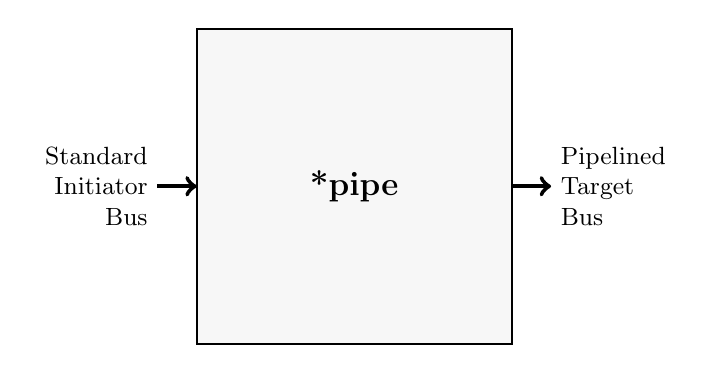
\begin{tikzpicture}
      %Block
      \draw [thick, fill=gray!6] (4,0) rectangle (8,4);
      \node at (6,2)
            {\begin{minipage}[c]{8em}
                \begin{center}
                  \hyphenchar\font=-1
                  \large{\textbf{\nameref*{pipe}}}
                \end{center}
             \end{minipage}};
      %Inputs     
      \node [left] at (3.5,2)
            {\begin{minipage}[c]{4em}
                \begin{flushright}
                  \hyphenchar\font=-1
                  \small{Standard Initiator Bus}
                \end{flushright}
             \end{minipage}};
      \draw [ultra thick, ->] (3.5,2) -- (4,2);
      %Outputs     
      \node [right] at (8.5,2)
            {\begin{minipage}[c]{4em}
                \begin{flushleft}
                  \hyphenchar\font=-1
                  \small{Pipelined Target Bus}
                \end{flushleft}
             \end{minipage}};
      \draw [ultra thick, ->] (8,2) -- (8.5,2);
    \end{tikzpicture}
    \caption{Block Diagram of the \nameref*{pipe}}
    \label{pipe:diag}
  \end{center}
\end{figure}
  
\subsubsection{Integration Parameters}
\label{pipe:param}

The \nameref*{pipe} supports the integration parameters listed in \tabref{pipe:param:tab}. 
See \secref{param} for a detailed description of all integration parameters.

\begin{center}
  \rowcolors{1}{gray!12}{white}                                         %set alternating row color
  \begin{longtable}{|l|r|l|}
    \rowcolor{white}
    \caption{Integration Parameters of the \nameref*{pipe}}
    \label{pipe:param:tab} \\
    %Header
    \hline                                     
    \rowcolor{gray!25}
    \multicolumn{1}{|c|}{\textbf{\rule{0pt}{2.5ex} Parameter}}  &  
    \multicolumn{1}{c|}{\textbf{\rule{0pt}{2.5ex}  Default}}    & 
    \multicolumn{1}{c|}{\textbf{\rule{0pt}{2.5ex}  Decription}} \\
    \hline                                    
    \endhead                               
    %Footers
    \hline
    \rowcolor{white}
    \multicolumn{3}{r}{\tiny{...continued}} \\
    \endfoot
    \hline
    \endlastfoot
    %Content
    \texttt{ADR\_WIDTH}       & \texttt{16} & Width of the address bus             \\
    \texttt{DAT\_WIDTH}       & \texttt{16} & Width of each data bus               \\
    \texttt{SEL\_WIDTH }      & \texttt{2}  & Number of data select lines          \\
    \texttt{TGA\_WIDTH }      & \texttt{1}  & Number of address tags               \\
    \texttt{TGC\_WIDTH }      & \texttt{1}  & Number of cycle tags                 \\
    \texttt{TGRD\_WIDTH}      & \texttt{1}  & Number of read data tags             \\
    \texttt{TGWD\_WIDTH}      & \texttt{1}  & Number of write data tags            \\
  \end{longtable}
\end{center}

\subsubsection{Interface Signals}
\label{pipe:sig}

\tabref{pipe:sig:tab} lists the interface signals of the \nameref*{pipe}. 
See \secref{sig} for a detailed description of all interface signals.

\begin{center}
  \rowcolors{1}{gray!12}{white}                                         %set alternating row color
  \begin{longtable}{|l|r|l|l|}
    \rowcolor{white}
    \caption{Interface Signals of the \nameref*{pipe}}
    \label{pipe:sig:tab} \\
    %Header
    \hline
    \rowcolor{gray!25}
    \multicolumn{1}{|c|}{\textbf{\rule{0pt}{2.5ex} Signal}}     &  
    \multicolumn{1}{c|}{\textbf{\rule{0pt}{2.5ex}  Range}}      & 
    \multicolumn{1}{c|}{\textbf{\rule{0pt}{2.5ex}  Direction}}  & 
    \multicolumn{1}{c|}{\textbf{\rule{0pt}{2.5ex}  Decription}} \\
    \hline
    \endhead                               
    %Footers
    \hline
    \rowcolor{white}
    \multicolumn{4}{r}{\tiny{...continued}} \\
    \endfoot
    \hline
    \endlastfoot
     %Section 'Clock and Reset'
    %\hline
    \rowcolor{gray!20}
    \multicolumn{4}{|c|}{\scriptsize{\rule{0pt}{2.5ex} Clock and Reset}} \global\rownum=1\relax  \\*  
    \nobreakhline
    \texttt{clk\_i}        &                                & input  & module    clock           \\*
    \texttt{async\_rst\_i} &                                & input  & asynchronous reset        \\*
    \texttt{sync\_rst\_i}  &                                & input  & synchronous reset         \\
    %Section 'Initiator Interface'
    \hline                                 
    \rowcolor{gray!20}
    \multicolumn{4}{|c|}{\scriptsize{\rule{0pt}{2.5ex} Initiator Interface}} \global\rownum=1\relax \\    
    \hline                                 
    \texttt{itr\_cyc\_i}   &                                & input  & bus cycle indicator       \\
    \texttt{itr\_stb\_i}   &                                & input  & access request            \\
    \texttt{itr\_we\_i}    &                                & input  & write enable              \\
    \texttt{itr\_lock\_i}  &                                & input  & uninterruptable bus cycle \\
    \texttt{itr\_sel\_i}   & \texttt{SEL\_WIDTH-1:0}        & input  & write data selects        \\
    \texttt{itr\_adr\_i}   & \texttt{ADR\_WIDTH-1:0}        & input  & address bus               \\
    \texttt{itr\_dat\_i}   & \texttt{DAT\_WIDTH-1:0}        & input  & write data bus            \\
    \texttt{itr\_tga\_i}   & \texttt{TGA\_WIDTH-1:0}        & input  & address tags              \\
    \texttt{itr\_tgc\_i}   & \texttt{TGC\_WIDTH-1:0}        & input  & bus cycle tags            \\
    \texttt{itr\_tgd\_i}   & \texttt{TGWD\_WIDTH-1:0}       & input  & write data tags           \\
    \texttt{itr\_ack\_o}   &                                & output & bus cycle acknowledge     \\
    \texttt{itr\_err\_o}   &                                & output & error indicator           \\
    \texttt{itr\_rty\_o}   &                                & output & retry request             \\
    \texttt{itr\_stall\_o} &                                & output & access delay              \\
    \texttt{itr\_dat\_o}   & \texttt{DAT\_WIDTH-1:0}        & output & read data bus             \\
    \texttt{itr\_tgd\_o}   & \texttt{TGRD\_WIDTH-1:0}       & output & read data tags            \\ 
    %Section 'Target Interface'
    \hline                                                                                      
    \rowcolor{gray!20}
    \multicolumn{4}{|c|}{\scriptsize{\rule{0pt}{2.5ex} Target Interface}} \global\rownum=1\relax \\  
    \hline                                                                                      
    \texttt{tgt\_cyc\_o}         &                          & output & bus cycle indicator       \\
    \texttt{tgt\_stb\_o}         &                          & output & access request            \\
    \texttt{tgt\_we\_o}          &                          & output & write enable              \\
    \texttt{tgt\_lock\_o}        &                          & output & uninterruptable bus cycle \\
    \texttt{tgt\_sel\_o}         & \texttt{SEL\_WIDTH-1:0}  & output & write data selects        \\
    \texttt{tgt\_adr\_o}         & \texttt{ADR\_WIDTH-1:0}  & output & write data selects        \\
    \texttt{tgt\_dat\_o}         & \texttt{DAT\_WIDTH-1:0}  & output & write data bus            \\
    \texttt{tgt\_tga\_o}         & \texttt{TGA\_WIDTH-1:0}  & output & address tags              \\
    \texttt{tgt\_tgc\_o}         & \texttt{TGC\_WIDTH-1:0}  & output & bus cycle tags            \\
    \texttt{tgt\_tgd\_o}         & \texttt{TGWD\_WIDTH-1:0} & output & write data tags           \\
    \texttt{tgt\_ack\_i}         &                          & input  & bus cycle acknowledge     \\
    \texttt{tgt\_err\_i}         &                          & input  & error indicator           \\
    \texttt{tgt\_rty\_i}         &                          & input  & retry request             \\
    \texttt{tgt\_stall\_i}       &                          & input  & access delay              \\
    \texttt{tgt\_dat\_i}         & \texttt{DAT\_WIDTH-1:0}  & input  & read data bus             \\
    \texttt{tgt\_tgd\_i}         & \texttt{TGRD\_WIDTH-1:0} & input  & read data tags            \\   
  \end{longtable}
\end{center}  

\subsubsection{Verification Status}
\label{pipe:verif}

\tabref[Table]{pipe:verif:tab} provides an overview of the verification status of the \nameref*{pipe}.
Lint checks have been done with the Icarus Verilog simulator~\cite{iverilog} and the Yosys synthesis tool~\cite{yosys}.

\begin{center}
  \rowcolors{1}{gray!12}{white}                                         %set alternating row color
  \begin{longtable}{|lr|c|c|c|c|}
    \rowcolor{white}
    \caption[Interface Signals]{Verification Status of the \nameref*{pipe}}
    \label{pipe:verif:tab} \\
    %Header
    \hline                              
    \rowcolor{gray!25}
    \multicolumn{2}{|c|}{\textbf{\rule{0pt}{2.5ex} Configuration}} &  
    \multicolumn{1}{c|}{\textbf{\rule{0pt}{2.5ex}  Linting}}       &  
    \multicolumn{1}{c|}{\textbf{\rule{0pt}{2.5ex}  Simulation}}    &  
    \multicolumn{1}{c|}{\textbf{\rule{0pt}{2.5ex}  Formal}}        &  
    \multicolumn{1}{c|}{\textbf{\rule{0pt}{2.5ex}  FPGA}}          \\
    \hline                              
    \endhead                               
    %Footers
    \hline
    \rowcolor{white}
    \multicolumn{6}{r}{\tiny{...continued}} \\
    \endfoot
    \hline
    \endlastfoot
    %Content
    \makecell[l]{\underline{\smash{\texttt{default}:}} \\ 
                 \texttt{ADR\_WIDTH}        \\
                 \texttt{DAT\_WIDTH}        \\
                 \texttt{SEL\_WIDTH}        \\
                 \texttt{TGA\_WIDTH}        \\
                 \texttt{TGC\_WIDTH}        \\
                 \texttt{TGRD\_WIDTH}       \\
                 \texttt{TGWD\_WIDTH}} &  
    \makecell[r]{                           \\ 
                 \texttt{16}                \\
                 \texttt{16}                \\
                 \texttt{2}                 \\
                 \texttt{1}                 \\
                 \texttt{1}                 \\
                 \texttt{1}                 \\
                 \texttt{1}}             &      
    \makecell[c]{iVerilog~\cite{iverilog}   \\                    
                 Yosis~\cite{yosys}}     &
    & & \\
  \end{longtable}
\end{center}
  


%###############################################################################
%# WbXbc - Manual - Pipelined to Standard Bus Gasket                           #
%###############################################################################
%#    Copyright 2018 Dirk Heisswolf                                            #
%#    This file is part of the WbXbc project.                                  #
%#                                                                             #
%#    WbXbc is free software: you can redistribute it and/or modify            #
%#    it under the terms of the GNU General Public License as published by     #
%#    the Free Software Foundation, either version 3 of the License, or        #
%#    (at your option) any later version.                                      #
%#                                                                             #
%#    WbXbc is distributed in the hope that it will be useful,                 #
%#    but WITHOUT ANY WARRANTY; without even the implied warranty of           #
%#    MERCHANTABILITY or FITNESS FOR A PARTICULAR PURPOSE.  See the            #
%#    GNU General Public License for more details.                             #
%#                                                                             #
%#    You should have received a copy of the GNU General Public License        #
%#    along with WbXbc.  If not, see <http://www.gnu.org/licenses/>.           #
%###############################################################################
%# Version History:                                                            #
%#   October 1, 2018                                                           #
%#      - Initial release                                                      #
%###############################################################################

\subsection[WbXbc Standardizer]{WbXbc Standardizer (\texttt{WbXbc\_standardizer})}
\label{stand}

This module connects a pipelined Wishbone initiator to a standard
protocol target (see \figref{stand:diag}).                                                 
%               +-------------------+             
%               |                   |             
%               |                   |             
% Pipelined     |    WbXbc          |     Standard 
% Initiator --->|    Standardizer   +---> Target  
% Bus           |                   |     Bus    
%               |                   |           
%               |                   |             
%               +-------------------+             
\begin{figure}[!h]
  \begin{center}
    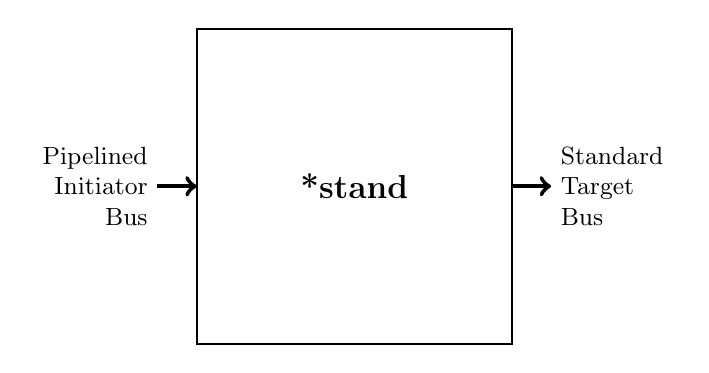
\begin{tikzpicture}
      %Block
      \draw [thick, fill=white] (4,0) rectangle (8,4);
      \node at (6,2)
            {\begin{minipage}[c]{8em}
                \begin{center}
                  \hyphenchar\font=-1
                  \large{\textbf{\nameref*{stand}}}
                \end{center}
             \end{minipage}};
      %Inputs     
      \node [left] at (3.5,2)
            {\begin{minipage}[c]{4em}
                \begin{flushright}
                  \hyphenchar\font=-1
                  \small{Pipelined Initiator Bus}
                \end{flushright}
             \end{minipage}};
      \draw [ultra thick, ->] (3.5,2) -- (4,2);
      %Outputs     
      \node [right] at (8.5,2)
            {\begin{minipage}[c]{4em}
                \begin{flushleft}
                  \hyphenchar\font=-1
                  \small{Standard Target Bus}
                \end{flushleft}
             \end{minipage}};
      \draw [ultra thick, ->] (8,2) -- (8.5,2);
    \end{tikzpicture}
    \caption{Block Diagram of the \nameref*{stand}}
    \label{stand:diag}
  \end{center}
\end{figure}
  
\subsubsection{Integration Parameters}
\label{stand:param}

The \nameref*{stand} supports the integration parameters listed in \tabref{stand:param:tab}. 
See \secref{param} for a detailed description of all integration parameters.

\begin{center}
  \rowcolors{1}{gray!12}{white}                                         %set alternating row color
  \begin{longtable}{|l|r|l|}
    \rowcolor{white}
    \caption{Integration Parameters of the \nameref*{stand}}
    \label{stand:param:tab} \\
    %Header
    \hline                                     
    \rowcolor{gray!25}
    \multicolumn{1}{|c|}{\textbf{\rule{0pt}{2.5ex} Parameter}}  &  
    \multicolumn{1}{c|}{\textbf{\rule{0pt}{2.5ex}  Default}}    & 
    \multicolumn{1}{c|}{\textbf{\rule{0pt}{2.5ex}  Decription}} \\
    \hline                                    
    \endhead                               
    %Footers
    \hline
    \rowcolor{white}
    \multicolumn{3}{r}{\tiny{...continued}} \\
    \endfoot
    \hline
    \endlastfoot
    %Content
    \texttt{ADR\_WIDTH}       & \texttt{16} & Width of the address bus             \\
    \texttt{DAT\_WIDTH}       & \texttt{16} & Width of each data bus               \\
    \texttt{SEL\_WIDTH }      & \texttt{2}  & Number of data select lines          \\
    \texttt{TGA\_WIDTH }      & \texttt{1}  & Number of address tags               \\
    \texttt{TGC\_WIDTH }      & \texttt{1}  & Number of cycle tags                 \\
    \texttt{TGRD\_WIDTH}      & \texttt{1}  & Number of read data tags             \\
    \texttt{TGWD\_WIDTH}      & \texttt{1}  & Number of write data tags            \\
  \end{longtable}
\end{center}

\subsubsection{Interface Signals}
\label{stand:sig}

\tabref{stand:sig:tab} lists the interface signals of the \nameref*{stand}. 
See \secref{sig} for a detailed description of all interface signals.

\begingroup
\setlength{\LTleft}{-20cm plus -1fill}
\setlength{\LTright}{\LTleft}
\begin{center}
  \rowcolors{1}{gray!12}{white}                                         %set alternating row color
  \begin{longtable}{|l|r|l|l|}
    \rowcolor{white}
    \caption{Interface Signals of the \nameref*{stand}}
    \label{stand:sig:tab} \\
    %Header
    \hline                                     
    \rowcolor{gray!25}
    \multicolumn{1}{|c|}{\textbf{\rule{0pt}{2.5ex} Signal}}     &  
    \multicolumn{1}{c|}{\textbf{\rule{0pt}{2.5ex}  Range}}      & 
    \multicolumn{1}{c|}{\textbf{\rule{0pt}{2.5ex}  Direction}}  & 
    \multicolumn{1}{c|}{\textbf{\rule{0pt}{2.5ex}  Decription}} \\
    \hline
    \endhead                               
    %Footers
    \hline
    \rowcolor{white}
    \multicolumn{4}{r}{\tiny{...continued}} \\
    \endfoot
    \hline
    \endlastfoot
     %Section 'Clock and Reset'
    %\hline
    \rowcolor{gray!20}
    \multicolumn{4}{|c|}{\scriptsize{\rule{0pt}{2.5ex} Clock and Reset}} \global\rownum=1\relax  \\*  
    \nobreakhline                                                                                       
    \texttt{clk\_i}        &                                & input  & module    clock           \\*
    \texttt{async\_rst\_i} &                                & input  & asynchronous reset        \\*
    \texttt{sync\_rst\_i}  &                                & input  & synchronous reset         \\
    %Section 'Initiator Interface'
    \hline                                 
    \rowcolor{gray!20}
    \multicolumn{4}{|c|}{\scriptsize{\rule{0pt}{2.5ex} Initiator Interface}} \global\rownum=1\relax \\*    
    \nobreakhline                                 
    \texttt{itr\_cyc\_i}   &                                & input  & bus cycle indicator          \\*
    \texttt{itr\_stb\_i}   &                                & input  & access request               \\*
    \texttt{itr\_we\_i}    &                                & input  & write enable                 \\*
    \texttt{itr\_lock\_i}  &                                & input  & uninterruptable bus cycle    \\*
    \texttt{itr\_sel\_i}   & \texttt{SEL\_WIDTH-1:0}        & input  & write data selects           \\*
    \texttt{itr\_adr\_i}   & \texttt{ADR\_WIDTH-1:0}        & input  & address bus                  \\*
    \texttt{itr\_dat\_i}   & \texttt{DAT\_WIDTH-1:0}        & input  & write data bus               \\*
    \texttt{itr\_tga\_i}   & \texttt{TGA\_WIDTH-1:0}        & input  & address tags                 \\*
    \texttt{itr\_tgc\_i}   & \texttt{TGC\_WIDTH-1:0}        & input  & bus cycle tags               \\*
    \texttt{itr\_tgd\_i}   & \texttt{TGWD\_WIDTH-1:0}       & input  & write data tags              \\*
    \texttt{itr\_ack\_o}   &                                & output & bus cycle acknowledge        \\*
    \texttt{itr\_err\_o}   &                                & output & error indicator              \\*
    \texttt{itr\_rty\_o}   &                                & output & retry request                \\*
    \texttt{itr\_stall\_o} &                                & output & access delay                 \\*
    \texttt{itr\_dat\_o}   & \texttt{DAT\_WIDTH-1:0}        & output & read data bus                \\*
    \texttt{itr\_tgd\_o}   & \texttt{TGRD\_WIDTH-1:0}       & output & read data tags               \\ 
    %Section 'Target Interface'
    \hline                                                                                      
    \rowcolor{gray!20}
    \multicolumn{4}{|c|}{\scriptsize{\rule{0pt}{2.5ex} Target Interface}} \global\rownum=1\relax \\  
    \nobreakhline                                                                                      
    \texttt{tgt\_cyc\_o}         &                          & output & bus cycle indicator       \\
    \texttt{tgt\_stb\_o}         &                          & output & access request            \\
    \texttt{tgt\_we\_o}          &                          & output & write enable              \\
    \texttt{tgt\_lock\_o}        &                          & output & uninterruptable bus cycle \\
    \texttt{tgt\_sel\_o}         & \texttt{SEL\_WIDTH-1:0}  & output & write data selects        \\
    \texttt{tgt\_adr\_o}         & \texttt{ADR\_WIDTH-1:0}  & output & write data selects        \\
    \texttt{tgt\_dat\_o}         & \texttt{DAT\_WIDTH-1:0}  & output & write data bus            \\
    \texttt{tgt\_tga\_o}         & \texttt{TGA\_WIDTH-1:0}  & output & address tags              \\
    \texttt{tgt\_tgc\_o}         & \texttt{TGC\_WIDTH-1:0}  & output & bus cycle tags            \\
    \texttt{tgt\_tgd\_o}         & \texttt{TGWD\_WIDTH-1:0} & output & write data tags           \\
    \texttt{tgt\_ack\_i}         &                          & input  & bus cycle acknowledge     \\
    \texttt{tgt\_err\_i}         &                          & input  & error indicator           \\
    \texttt{tgt\_rty\_i}         &                          & input  & retry request             \\
    \texttt{tgt\_stall\_i}       &                          & input  & access delay              \\
    \texttt{tgt\_dat\_i}         & \texttt{DAT\_WIDTH-1:0}  & input  & read data bus             \\
    \texttt{tgt\_tgd\_i}         & \texttt{TGRD\_WIDTH-1:0} & input  & read data tags            \\   
  \end{longtable}
\end{center}  
\endgroup

\subsubsection{Verification Status}
\label{stand:verif}

\tabref[Table]{stand:verif:tab} provides an overview of the verification status of the \nameref*{stand}.
Lint checks have been done with the Icarus Verilog simulator~\cite{iverilog} and the Yosys synthesis tool~\cite{yosys}.

\begin{center}
  \rowcolors{1}{gray!12}{white}                                         %set alternating row color
  \begin{longtable}{|lr|c|c|c|c|}
    \rowcolor{white}
    \caption[Interface Signals]{Verification Status of the \nameref*{stand}}
    \label{stand:verif:tab} \\
    %Header
    \hline                              
    \rowcolor{gray!25}
    \multicolumn{2}{|c|}{\textbf{\rule{0pt}{2.5ex} Configuration}} &  
    \multicolumn{1}{c|}{\textbf{\rule{0pt}{2.5ex}  Linting}}       &  
    \multicolumn{1}{c|}{\textbf{\rule{0pt}{2.5ex}  Simulation}}    &  
    \multicolumn{1}{c|}{\textbf{\rule{0pt}{2.5ex}  Formal}}        &  
    \multicolumn{1}{c|}{\textbf{\rule{0pt}{2.5ex}  FPGA}}          \\
    \hline                              
    \endhead                               
    %Footers
    \hline
    \rowcolor{white}
    \multicolumn{6}{r}{\tiny{...continued}} \\
    \endfoot
    \hline
    \endlastfoot
    %Content
    \makecell[l]{Default:                   \\ 
                 \texttt{ADR\_WIDTH}        \\
                 \texttt{DAT\_WIDTH}        \\
                 \texttt{SEL\_WIDTH}        \\
                 \texttt{TGA\_WIDTH}        \\
                 \texttt{TGC\_WIDTH}        \\
                 \texttt{TGRD\_WIDTH}       \\
                 \texttt{TGWD\_WIDTH}} &  
    \makecell[r]{                           \\ 
                 \texttt{16}                \\
                 \texttt{16}                \\
                 \texttt{2}                 \\
                 \texttt{1}                 \\
                 \texttt{1}                 \\
                 \texttt{1}                 \\
                 \texttt{1}}             &      
    \makecell[c]{iVerilog~\cite{iverilog}   \\                    
                 Yosis~\cite{yosys}}     &
    & & \\
  \end{longtable}
\end{center}
  


%###############################################################################
%# WbXbc - Manual - Bus Distributor                                            #
%###############################################################################
%#    Copyright 2018 Dirk Heisswolf                                            #
%#    This file is part of the WbXbc project.                                  #
%#                                                                             #
%#    WbXbc is free software: you can redistribute it and/or modify            #
%#    it under the terms of the GNU General Public License as published by     #
%#    the Free Software Foundation, either version 3 of the License, or        #
%#    (at your option) any later version.                                      #
%#                                                                             #
%#    WbXbc is distributed in the hope that it will be useful,                 #
%#    but WITHOUT ANY WARRANTY; without even the implied warranty of           #
%#    MERCHANTABILITY or FITNESS FOR A PARTICULAR PURPOSE.  See the            #
%#    GNU General Public License for more details.                             #
%#                                                                             #
%#    You should have received a copy of the GNU General Public License        #
%#    along with WbXbc.  If not, see <http://www.gnu.org/licenses/>.           #
%###############################################################################
%# Version History:                                                            #
%#   October 1, 2018                                                           #
%#      - Initial release                                                      #
%###############################################################################

\subsection[WbXbc Distributor]{WbXbc Distributor (\texttt{WbXbc\_distributor})}
\label{dist}

This module combines an \hyperref{adec}{address decoder}, an \hyperref{errgen}{error generator},
and a \hyperref{split}{bus splitter} for the pipelined Wishbone protocol (see \figref{dist:diag}). 
%             +-------------------------------------------------------------------------------+         
%             |                                                                               |
%             |                               WbXbc Distributor                               |
%             |                                                                               |
%             |    +-------------------+    +-------------------+    +-------------------+    |             
% Address --->|--->|                   |    |                   |    |                   +--->|--->         
% Regions     |    |                   |    |                   |    |                   |    |             
%             |    |      WbXbc        |    |     WbXbc         |    |      WbXbc        +--->|---> Multiple
% Initiator   |    |      Address      +--->|     Error         +--->|      Splitter     |    |     Target 
% Bus     --->|--->|      Decoder      |    |     Generator     |    |                   | ...| ... Busses 
%             |    |                   |    |                   |    |                   |    |             
%             |    |                   |    |                   |    |                   +--->|--->         
%             |    +-------------------+    +-------------------+    +-------------------+    |             
%             |                                                                               |
%             +-------------------------------------------------------------------------------+        

\begin{figure}[!h]
  %\begin{center}
  \makebox[\textwidth][c]{
    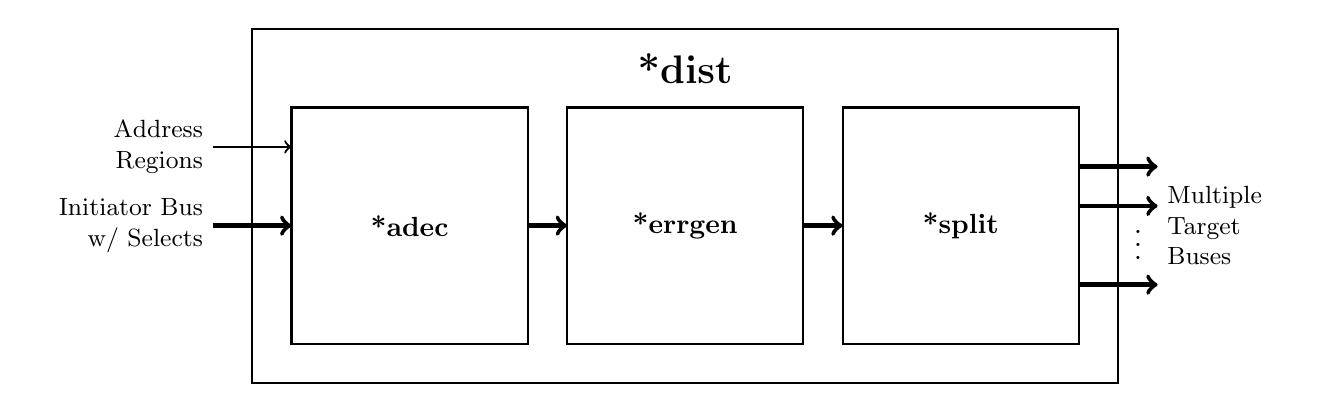
\begin{tikzpicture}
      %Block
      \draw [thick, fill=white] (4,0) rectangle (15,4.5);
      \node at (9.5,4)
            {\begin{minipage}[c]{16em}
                \begin{center}
                  \hyphenchar\font=-1
                  \Large{\textbf{\nameref*{dist}}}
                \end{center}
             \end{minipage}};
      %Inputs     
      \node [left] at (3.5,3)
            {\begin{minipage}[c]{6em}
                \begin{flushright}
                  \hyphenchar\font=-1
                  \small{Address Regions}
                \end{flushright}
             \end{minipage}};
      \draw [thick, ->] (3.5,3) -- (4.5,3);
      \node [left] at (3.5,2)
            {\begin{minipage}[c]{6em}
                \begin{flushright}
                  \hyphenchar\font=-1
                  \small{Initiator Bus w/ Selects}
                \end{flushright}
             \end{minipage}};
      \draw [ultra thick, ->] (3.5,2) -- (4.5,2);
      %Outputs     
      \node [right] at (15.5,2)
            {\begin{minipage}[c]{5em}
                \begin{flushleft}
                  \hyphenchar\font=-1
                  \small{Multiple Target Buses}
                \end{flushleft}
             \end{minipage}};
      \draw [ultra thick, ->] (14.5,2.75) -- (15.5,2.75);
      \draw [ultra thick, ->] (14.5,2.25) -- (15.5,2.25);
      \node [rotate=90] at (15.25,1.75) {\small{\texttt{...}}};
      \draw [ultra thick, ->] (14.5,1.25) -- (15.5,1.25);
      %Address decoder block  
      \draw [thick, fill=white] (4.5,0.5) rectangle (7.5,3.5);
      \node at (6,2)
            {\begin{minipage}[c]{8em}
                \begin{center}
                  \hyphenchar\font=-1
                  \textbf{\nameref*{adec}}
                \end{center}
             \end{minipage}};
      \draw [ultra thick, ->] (7.5,2) -- (8,2);
      %Error generator block  
      \draw [thick, fill=white] (8,0.5) rectangle (11,3.5);
      \node at (9.5,2)
            {\begin{minipage}[c]{8em}
                \begin{center}
                  \hyphenchar\font=-1
                  \textbf{\nameref*{errgen}}
                \end{center}
             \end{minipage}};
      %Splitter block  
      \draw [thick, fill=white] (11.5,0.5) rectangle (14.5,3.5);
      \node at (13,2)
            {\begin{minipage}[c]{8em}
                \begin{center}
                  \hyphenchar\font=-1
                  \textbf{\nameref*{split}}
                \end{center}
             \end{minipage}};
      \draw [ultra thick, ->] (11,2) -- (11.5,2);
    \end{tikzpicture}
    }
    \caption{Block Diagram of the \nameref*{dist}}
    \label{dist:diag}
  %\end{center}
\end{figure}

\subsubsection{Integration Parameters}
\label{dist:param}

The \nameref*{dist} supports the integration parameters listed in \tabref{dist:param:tab}. 
See \secref{param} for a detailed description of all integration parameters.

\begin{center}
  \rowcolors{1}{gray!12}{white}                                         %set alternating row color
  \begin{longtable}{|l|r|l|}
    \rowcolor{white}
    \caption{Integration Parameters of the \nameref*{dist}}
    \label{dist:param:tab} \\
    %Header
    \hline                                     
    \rowcolor{gray!25}
    \multicolumn{1}{|c|}{\textbf{\rule{0pt}{2.5ex} Parameter}}  &  
    \multicolumn{1}{c|}{\textbf{\rule{0pt}{2.5ex}  Default}}    & 
    \multicolumn{1}{c|}{\textbf{\rule{0pt}{2.5ex}  Decription}} \\
    \hline                                    
    \endhead                               
    %Footers
    \hline
    \rowcolor{white}
    \multicolumn{3}{r}{\tiny{...continued}} \\
    \endfoot
    \hline
    \endlastfoot
    %Content
    \texttt{TGT\_CNT   } & \texttt{4}  & Number of target busses              \\
    \texttt{ADR\_WIDTH}  & \texttt{16} & Width of the address bus             \\
    \texttt{DAT\_WIDTH}  & \texttt{16} & Width of each data bus               \\
    \texttt{SEL\_WIDTH } & \texttt{2}  & Number of data select lines          \\
    \texttt{TGA\_WIDTH } & \texttt{1}  & Number of address tags               \\
    \texttt{TGC\_WIDTH } & \texttt{1}  & Number of cycle tags                 \\
    \texttt{TGRD\_WIDTH} & \texttt{1}  & Number of read data tags             \\
    \texttt{TGWD\_WIDTH} & \texttt{1}  & Number of write data tags            \\
  \end{longtable}
\end{center}

\subsubsection{Interface Signals}
\label{dist:sig}

\tabref{dist:sig:tab} lists the interface signals of the \nameref*{dist}. 
See \secref{sig} for a detailed description of all interface signals.

\begingroup
\setlength{\LTleft}{-20cm plus -1fill}
\setlength{\LTright}{\LTleft}
\begin{center}
  \rowcolors{1}{gray!12}{white}                                         %set alternating row color
  \begin{longtable}{|l|r|l|l|}
    \rowcolor{white}
    \caption{Interface Signals of the \nameref*{dist}}
    \label{dist:sig:tab} \\
    %Header
    \hline                                     
    \rowcolor{gray!25}
    \multicolumn{1}{|c|}{\textbf{\rule{0pt}{2.5ex} Signal}}     &  
    \multicolumn{1}{c|}{\textbf{\rule{0pt}{2.5ex}  Range}}      & 
    \multicolumn{1}{c|}{\textbf{\rule{0pt}{2.5ex}  Direction}}  & 
    \multicolumn{1}{c|}{\textbf{\rule{0pt}{2.5ex}  Decription}} \\
    \hline
    \endhead                               
    %Footers
    \hline
    \rowcolor{white}
    \multicolumn{4}{r}{\tiny{...continued}} \\
    \endfoot
    \hline
    \endlastfoot
    %Section 'Clock and Reset'
    %\hline
    \rowcolor{gray!20}
    \multicolumn{4}{|c|}{\scriptsize{\rule{0pt}{2.5ex} Clock and Reset}} \global\rownum=1\relax \\  
    \hline                                    
    \texttt{clk\_i}        &                                & input & module clock              \\
    \texttt{async\_rst\_i} &                                & input & asynchronous reset        \\
    \texttt{sync\_rst\_i}  &                                & input & synchronous reset         \\
    %Section 'Target Address Regions'
    %\hline
    \rowcolor{gray!20}
    \multicolumn{4}{|c|}{\scriptsize{\rule{0pt}{2.5ex} Target Address Regions}} \global\rownum=1\relax \\  
    \hline                                    
    \texttt{region\_adr\_i} & \texttt{(TGT\_CNT*ADR\_WIDTH)\-1:0} & input & target address regions                     \\
    \texttt{region\_msk\_i} & \texttt{(TGT\_CNT*ADR\_WIDTH)\-1:0} & input & \makecell[l]{selects relevant address bits \\
                                                                                         (1: relevant, 0: ignored)}    \\
    %Section 'Initiator Interface'
    \hline                                 
    \rowcolor{gray!20}
    \multicolumn{4}{|c|}{\scriptsize{\rule{0pt}{2.5ex} Initiator Interface}} \global\rownum=1\relax \\    
    \hline                                 
    \texttt{itr\_cyc\_i}   &                                & input  & bus cycle indicator       \\
    \texttt{itr\_stb\_i}   &                                & input  & access request            \\
    \texttt{itr\_we\_i}    &                                & input  & write enable              \\
    \texttt{itr\_lock\_i}  &                                & input  & uninterruptable bus cycle \\
    \texttt{itr\_sel\_i}   & \texttt{SEL\_WIDTH-1:0}        & input  & write data selects        \\
    \texttt{itr\_adr\_i}   & \texttt{ADR\_WIDTH-1:0}        & input  & address bus               \\
    \texttt{itr\_dat\_i}   & \texttt{DAT\_WIDTH-1:0}        & input  & write data bus            \\
    \texttt{itr\_tga\_i}   & \texttt{TGA\_WIDTH-1:0}        & input  & address tags              \\
    \texttt{itr\_tgc\_i}   & \texttt{TGC\_WIDTH-1:0}        & input  & bus cycle tags            \\
    \texttt{itr\_tgd\_i}   & \texttt{TGWD\_WIDTH-1:0}       & input  & write data tags           \\
    \texttt{itr\_ack\_o}   &                                & output & bus cycle acknowledge     \\
    \texttt{itr\_err\_o}   &                                & output & error indicator           \\
    \texttt{itr\_rty\_o}   &                                & output & retry request             \\
    \texttt{itr\_stall\_o} &                                & output & access delay              \\
    \texttt{itr\_dat\_o}   & \texttt{DAT\_WIDTH-1:0}        & output & read data bus             \\
    \texttt{itr\_tgd\_o}   & \texttt{TGRD\_WIDTH-1:0}       & output & read data tags            \\ 
    %Section 'Target Interface'
    \hline                                                                                      
    \rowcolor{gray!20}
    \multicolumn{4}{|c|}{\scriptsize{\rule{0pt}{2.5ex} Target Interface}} \global\rownum=1\relax \\  
    \hline                                                                                      
    \texttt{tgt\_cyc\_o}         & \texttt{TGT\_CNT-1:0}               & output & concatinated bus cycle indicators   \\
    \texttt{tgt\_stb\_o}         & \texttt{TGT\_CNT-1:0}               & output & concatinated access requests	      \\
    \texttt{tgt\_we\_o}          & \texttt{TGT\_CNT-1:0}               & output & concatinated write enables	      \\
    \texttt{tgt\_lock\_o}        & \texttt{TGT\_CNT-1:0}               & output & concatinated bus cycle locks	      \\
    \texttt{tgt\_sel\_o}         & \texttt{(TGT\_CNT*SEL\_WIDTH)-1:0}  & output & concatinated write data selects     \\
    \texttt{tgt\_adr\_o}         & \texttt{(TGT\_CNT*ADR\_WIDTH)-1:0}  & output & concatinated write data selects     \\
    \texttt{tgt\_dat\_o}         & \texttt{(TGT\_CNT*DAT\_WIDTH)-1:0}  & output & concatinated write data busses      \\
    \texttt{tgt\_tga\_o}         & \texttt{(TGT\_CNT*TGA\_WIDTH))-1:0} & output & concatinated address tags	      \\
    \texttt{tgt\_tgc\_o}         & \texttt{(TGT\_CNT*TGC\_WIDTH)-1:0}  & output & concatinated bus cycle tags	      \\
    \texttt{tgt\_tgd\_o}         & \texttt{(TGT\_CNT*TGWD\_WIDT)-1:0}  & output & concatinated write data tags	      \\
    \texttt{tgt\_ack\_i}         & \texttt{TGT\_CNT-1:0}               & input  & concatinated bus cycle acknowledges \\
    \texttt{tgt\_err\_i}         & \texttt{TGT\_CNT-1:0}               & input  & concatinated error indicators	      \\
    \texttt{tgt\_rty\_i}         & \texttt{TGT\_CNT-1:0}               & input  & concatinated retry requests	      \\
    \texttt{tgt\_stall\_i}       & \texttt{TGT\_CNT-1:0}               & input  & concatinated access delays	      \\
    \texttt{tgt\_dat\_i}         & \texttt{(TGT\_CNT*DAT\_WIDTH-1):0}  & input  & concatinated read data busses	      \\
    \texttt{tgt\_tgd\_i}         & \texttt{(TGT\_CNT*TGRD\_WIDTH-1):0} & input  & concatinated read data tags         \\   
  \end{longtable}
\end{center}  
\endgroup

\subsubsection{Verification Status}
\label{dist:verif}

\tabref[Table]{dist:verif:tab} provides an overview of the verification status of the \nameref*{dist}.
Lint checks have been done with the Icarus Verilog simulator~\cite{iverilog} and the Yosys synthesis tool~\cite{yosys}.

\begin{center}
  \rowcolors{1}{gray!12}{white}                                         %set alternating row color
  \begin{longtable}{|lr|c|c|c|c|}
    \rowcolor{white}
    \caption[Interface Signals]{Verification Status of the \nameref*{dist}}
    \label{dist:verif:tab} \\
    %Header
    \hline                              
    \rowcolor{gray!25}
    \multicolumn{2}{|c|}{\textbf{\rule{0pt}{2.5ex} Configuration}} &  
    \multicolumn{1}{c|}{\textbf{\rule{0pt}{2.5ex}  Linting}}       &  
    \multicolumn{1}{c|}{\textbf{\rule{0pt}{2.5ex}  Simulation}}    &  
    \multicolumn{1}{c|}{\textbf{\rule{0pt}{2.5ex}  Formal}}        &  
    \multicolumn{1}{c|}{\textbf{\rule{0pt}{2.5ex}  FPGA}}          \\
    \hline                              
    \endhead                               
    %Footers
    \hline
    \rowcolor{white}
    \multicolumn{6}{r}{\tiny{...continued}} \\
    \endfoot
    \hline
    \endlastfoot
    %Content
    \makecell[l]{\underline{\smash{\texttt{default}:}} \\ 
                 \texttt{TGT\_CNT}    \\
                 \texttt{ADR\_WIDTH}  \\
                 \texttt{DAT\_WIDTH}  \\
                 \texttt{SEL\_WIDTH}  \\
                 \texttt{TGA\_WIDTH}  \\
                 \texttt{TGC\_WIDTH}  \\
                 \texttt{TGRD\_WIDTH} \\
                 \texttt{TGWD\_WIDTH}}   &
    \makecell[r]{                     \\ 
                 \texttt{4}           \\
                 \texttt{16}          \\
                 \texttt{16}          \\
                 \texttt{2}           \\
                 \texttt{1}           \\
                 \texttt{1}           \\
                 \texttt{1}           \\
                 \texttt{1}}             &     
    \makecell[c]{iVerilog~\cite{iverilog} \\                    
                 Yosis~\cite{yosys}}     &
    & & \\
  \end{longtable}
\end{center}
  


%###############################################################################
%# WbXbc - Manual - Plain Crossbar Switch                                      #
%###############################################################################
%#    Copyright 2018 Dirk Heisswolf                                            #
%#    This file is part of the WbXbc project.                                  #
%#                                                                             #
%#    WbXbc is free software: you can redistribute it and/or modify            #
%#    it under the terms of the GNU General Public License as published by     #
%#    the Free Software Foundation, either version 3 of the License, or        #
%#    (at your option) any later version.                                      #
%#                                                                             #
%#    WbXbc is distributed in the hope that it will be useful,                 #
%#    but WITHOUT ANY WARRANTY; without even the implied warranty of           #
%#    MERCHANTABILITY or FITNESS FOR A PARTICULAR PURPOSE.  See the            #
%#    GNU General Public License for more details.                             #
%#                                                                             #
%#    You should have received a copy of the GNU General Public License        #
%#    along with WbXbc.  If not, see <http://www.gnu.org/licenses/>.           #
%###############################################################################
%# Version History:                                                            #
%#   October 1, 2018                                                           #
%#      - Initial release                                                      #
%###############################################################################

\subsection[WbXbc Xbar]{WbXbc Xbar (\texttt{WbXbc\_xbar})}
\label{xbar}

This module implements a full crossbar switch between a set of initator
busses and a set of target busses, all using the pipelined Wishbone    
protocol. The \nameref*{xbar} consists \hyperref[dist]{ditributor} and
\hyperref[arb]{arbiter} components (see \figref{xbar:diag}).                                                              
%      Initiator         Initiator            Initiator   
%          |                 |      . . .        |    
%          V                 V                   V    
% +----------------------------------------------------------------------+
% |        |                 |                   |                       | 
% |        V                 V                   V                       |
% |  +-----------+     +-----------+       +-----------+                 |
% |  |WbXbc      |     |WbXbc      |       |WbXbc      |                 |
% |  |Distributor|     |Distributor| . . . |Distributor|                 |
% |  +-+-+-----+-+     +-+-+-----+-+       +-+-+-----+-+                 |
% |    | | ... |         | | ... |           | | ... |                   |
% |    | |     |         | |     |           | |     |                   |
% |    | |     |         | |     |           | |     |     +---------+   |       
% |    +-|-----|---------|-|-----|-----------|-|-----|---->|         |   |       
% |      |     |         +-|---- |-----------|-|-----|---->| WbXbc   +-->|-->Target
% |      |     |           |     |           | |     | ... | Arbiter |   |       
% |      |     |           |     |           +-|-----|---->|         |   |       
% |      |     |           |     |             |     |     +---------+   |       
% |      |     |           |     |             |     |                   |       
% |      |     |           |     |             |     |     +---------+   |       
% |      +-----|-----------|-----|-------------|-----|---->|         |   |       
% |            |           +-----|-------------|-----|---->| WbXbc   +-->|-->Target
% |            |                 |             |     | ... | Arbiter |   |       
% |            |                 |             +-----|---->|         |   |       
% |            |                 |                   |     +---------+   |       
% |            |                 |                   |                   |       
% |            |                 |                   |        . . .      |   . . .       
% |            |                 |                   |                   |       
% |            |                 |                   |     +---------+   |       
% |            +-----------------|-------------------|---->|         |   |       
% |                              +-------------------|---->| WbXbc   +-->|-->Target
% |                                                  | ... | Arbiter |   |       
% |     WbXbc                                        +---->|         |   |       
% |     Xbar                                               +---------+   |  
% |                                                                      |
% +----------------------------------------------------------------------+
\begin{figure}[!h]
  %\begin{center}
  \makebox[\textwidth][c]{
    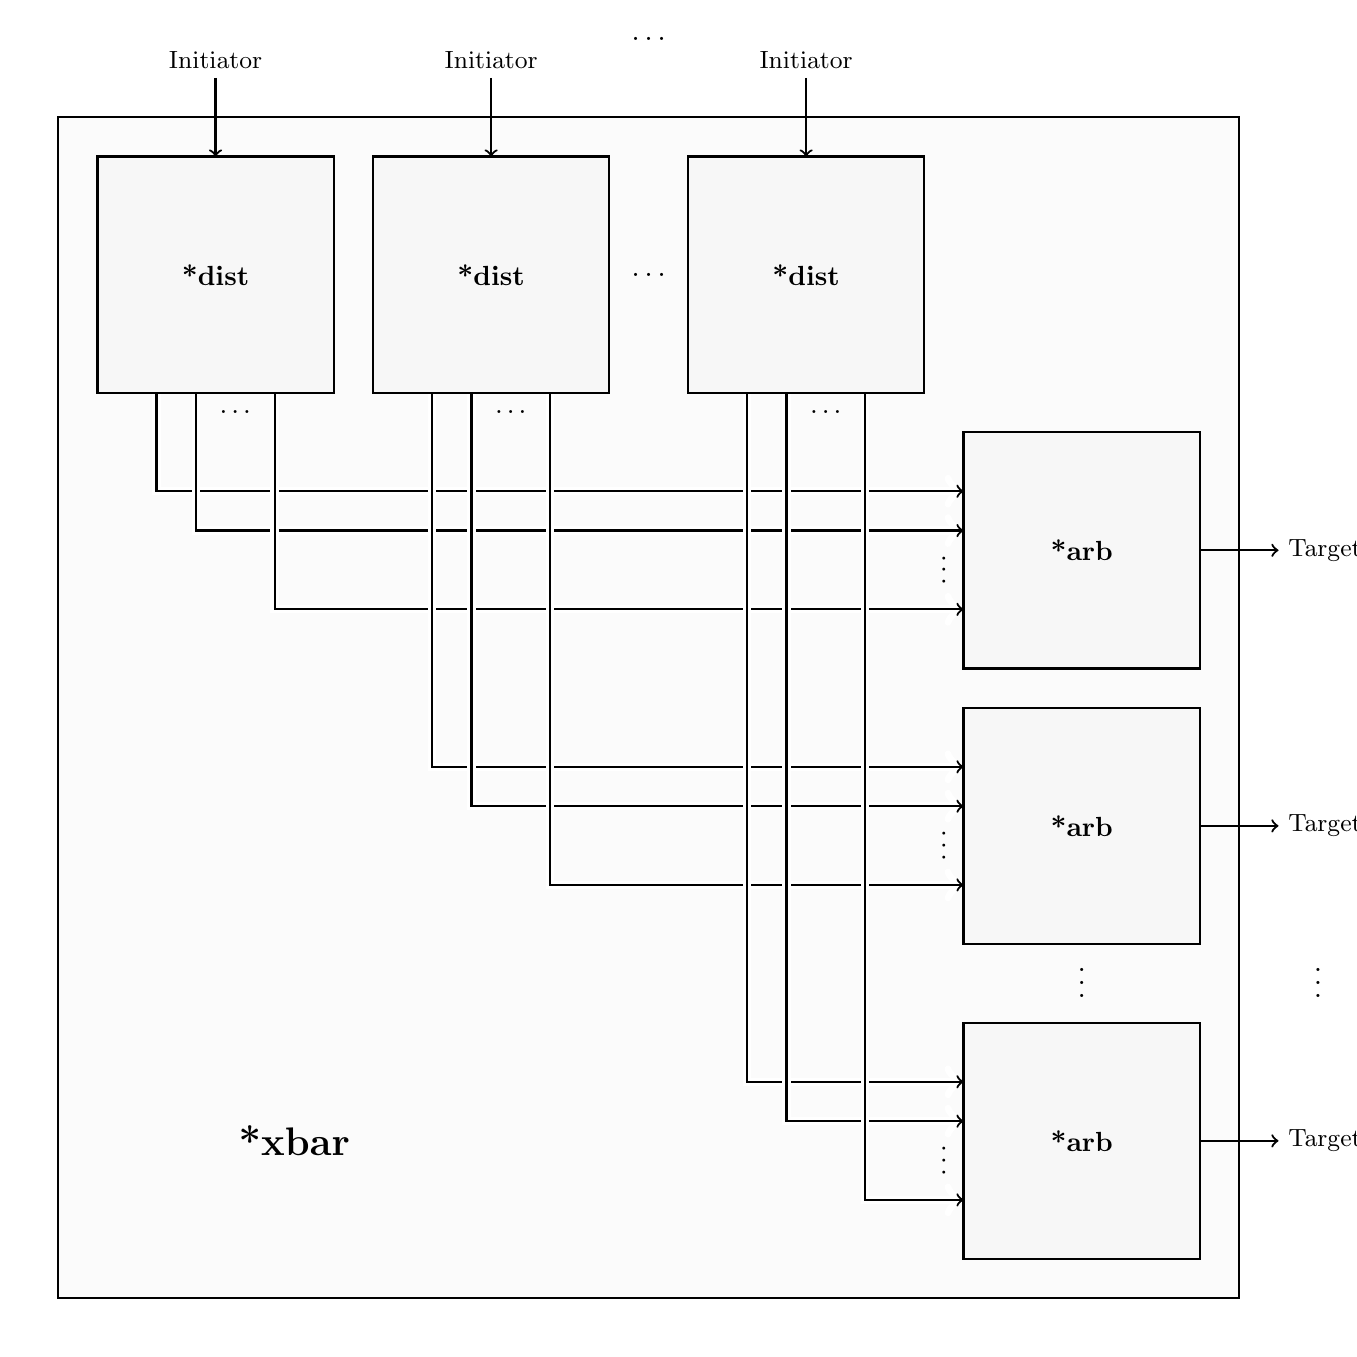
\begin{tikzpicture}
      %Block boundary
      \draw [thick, fill=gray!3] (0,0) rectangle (15,15);
      \node at (3,2)
            {\begin{minipage}[c]{16em}
                \begin{center}
                  \hyphenchar\font=-1
                  \Large{\textbf{\nameref*{xbar}}}
                \end{center}
            \end{minipage}};

      %Connections
      \draw [preaction={draw, line width=3pt, white}, thick, ->] ( 1.25,11.5) -- ( 1.25,10.25) -- (11.5,10.25);
      \draw [preaction={draw, line width=3pt, white}, thick, ->] ( 1.75,11.5) -- ( 1.75, 9.75) -- (11.5, 9.75);
      \draw [preaction={draw, line width=3pt, white}, thick, ->] ( 2.75,11.5) -- ( 2.75, 8.75) -- (11.5, 8.75);
             
      \draw [preaction={draw, line width=3pt, white}, thick, ->] ( 4.75,11.5) -- ( 4.75, 6.75) -- (11.5, 6.75);
      \draw [preaction={draw, line width=3pt, white}, thick, ->] ( 5.25,11.5) -- ( 5.25, 6.25) -- (11.5, 6.25);
      \draw [preaction={draw, line width=3pt, white}, thick, ->] ( 6.25,11.5) -- ( 6.25, 5.25) -- (11.5, 5.25);
             
      \draw [preaction={draw, line width=3pt, white}, thick, ->] ( 8.75,11.5) -- ( 8.75, 2.75) -- (11.5, 2.75);
      \draw [preaction={draw, line width=3pt, white}, thick, ->] ( 9.25,11.5) -- ( 9.25, 2.25) -- (11.5, 2.25);
      \draw [preaction={draw, line width=3pt, white}, thick, ->] (10.25,11.5) -- (10.25, 1.25) -- (11.5, 1.25);
      %Distributors
      \newsavebox{\distbox}
      \savebox{\distbox}{
        \draw [thick, fill=gray!6] (0,0) rectangle (3,3);
        \node at (1.5,1.5)
              {\begin{minipage}[c]{8em}
                  \begin{center}
                    \hyphenchar\font=-1
                    \textbf{\nameref*{dist}}
                  \end{center}
              \end{minipage}};
        \node [above] at (1.5,4)
              {\begin{minipage}[c]{4em}
                  \begin{center}
                    \hyphenchar\font=-1
                    \small{Initiator}
                  \end{center}
              \end{minipage}};
        \node at (1.75,-0.25) {\footnotesize{\texttt{...}}};
        \draw [thick, ->] (1.5,4) -- (1.5,3);}
      \node at (0.5,11.5) {\usebox{\distbox}};
      \node at (4,11.5)   {\usebox{\distbox}};
      \node at (7.5,13)   {\small{\texttt{...}}};
      \node at (7.5,16)   {\small{\texttt{...}}};
      \node at (8,11.5)   {\usebox{\distbox}}; 
      %Arbiters
      \newsavebox{\arbbox}
      \savebox{\arbbox}{
        \draw [thick, fill=gray!6] (0,0) rectangle (3,3);
        \node at (1.5,1.5)
              {\begin{minipage}[c]{8em}
                  \begin{center}
                    \hyphenchar\font=-1
                    \textbf{\nameref*{arb}}
                  \end{center}
              \end{minipage}};
        \node [right] at (4,1.5)
              {\begin{minipage}[c]{4em}
                  \begin{flushleft}
                    \hyphenchar\font=-1
                    \small{Target}
                  \end{flushleft}
              \end{minipage}};
        \node [rotate=90] at (-0.25,1.25) {\footnotesize{\texttt{...}}};
        \draw [thick, ->] (3,1.5) -- (4,1.5);}
      \node at (11.5,8)   {\usebox{\arbbox}};
      \node at (11.5,4.5) {\usebox{\arbbox}};
      \node [rotate=90] at (13,4) {\small{\texttt{...}}};
      \node [rotate=90] at (16,4) {\small{\texttt{...}}};
      \node at (11.5,0.5)   {\usebox{\arbbox}};
             
    \end{tikzpicture}
    }
    \caption{Block Diagram of the \nameref*{xbar}}
    \label{xbar:diag}
  %\end{center}
\end{figure}

\subsubsection{Integration Parameters}
\label{xbar:param}

The \nameref*{xbar} supports the integration parameters listed in \tabref{xbar:param:tab}. 
See \secref{param} for a detailed description of all integration parameters.

\begin{center}
  \rowcolors{1}{gray!12}{white}                                         %set alternating row color
  \begin{longtable}{|l|r|l|}
    \rowcolor{white}
    \caption{Integration Parameters of the \nameref*{xbar}}
    \label{xbar:param:tab} \\
    %Header
    \hline                                     
    \rowcolor{gray!25}
    \multicolumn{1}{|c|}{\textbf{\rule{0pt}{2.5ex} Parameter}}  &  
    \multicolumn{1}{c|}{\textbf{\rule{0pt}{2.5ex}  Default}}    & 
    \multicolumn{1}{c|}{\textbf{\rule{0pt}{2.5ex}  Decription}} \\
    \hline                                    
    \endhead                               
    %Footers
    \hline
    \rowcolor{white}
    \multicolumn{3}{r}{\tiny{...continued}} \\
    \endfoot
    \hline
    \endlastfoot
    %Content
    \texttt{ITR\_CNT   } & \texttt{4}  & Number of initiator busses           \\
    \texttt{TGT\_CNT   } & \texttt{4}  & Number of target busses              \\
    \texttt{ADR\_WIDTH } & \texttt{16} & Width of the address bus             \\
    \texttt{DAT\_WIDTH } & \texttt{16} & Width of each data bus               \\
    \texttt{SEL\_WIDTH } & \texttt{2}  & Number of data select lines          \\
    \texttt{TGA\_WIDTH } & \texttt{1}  & Number of address tags               \\
    \texttt{TGC\_WIDTH } & \texttt{1}  & Number of cycle tags                 \\
    \texttt{TGRD\_WIDTH} & \texttt{1}  & Number of read data tags             \\
    \texttt{TGWD\_WIDTH} & \texttt{1}  & Number of write data tags            \\
  \end{longtable}
\end{center}

\subsubsection{Interface Signals}
\label{xbar:sig}

\tabref{xbar:sig:tab} lists the interface signals of the \nameref*{xbar}. 
See \secref{sig} for a detailed description of all interface signals.

\begingroup
\setlength{\LTleft}{-20cm plus -1fill}
\setlength{\LTright}{\LTleft}
\begin{center}
  \rowcolors{1}{gray!12}{white}                                         %set alternating row color
  \begin{longtable}{|l|r|l|l|}
    \rowcolor{white}
    \caption{Interface Signals of the \nameref*{xbar}}
    \label{xbar:sig:tab} \\
    %Header
    \hline                                     
    \rowcolor{gray!25}
    \multicolumn{1}{|c|}{\textbf{\rule{0pt}{2.5ex} Signal}}     &  
    \multicolumn{1}{c|}{\textbf{\rule{0pt}{2.5ex}  Range}}      & 
    \multicolumn{1}{c|}{\textbf{\rule{0pt}{2.5ex}  Direction}}  & 
    \multicolumn{1}{c|}{\textbf{\rule{0pt}{2.5ex}  Decription}} \\
    \hline
    \endhead                               
    %Footers
    \hline
    \rowcolor{white}
    \multicolumn{4}{r}{\tiny{...continued}} \\
    \endfoot
    \hline
    \endlastfoot
    %Section 'Clock and Reset'
    %\hline
    \rowcolor{gray!20}
    \multicolumn{4}{|c|}{\scriptsize{\rule{0pt}{2.5ex} Clock and Reset}} \global\rownum=1\relax \\*  
    \nobreakhline                                    
    \texttt{clk\_i}        &                                & input & module clock              \\*
    \texttt{async\_rst\_i} &                                & input & asynchronous reset        \\*
    \texttt{sync\_rst\_i}  &                                & input & synchronous reset         \\
    %Section 'Target Address Regions'
    %\hline
    \rowcolor{gray!20}
    \multicolumn{4}{|c|}{\scriptsize{\rule{0pt}{2.5ex} Target Address Regions}} \global\rownum=1\relax                 \\*  
    \nobreakhline                                    
    \texttt{region\_adr\_i} & \texttt{(TGT\_CNT*ADR\_WIDTH)\-1:0} & input & target address                             \\*
    \texttt{region\_msk\_i} & \texttt{(TGT\_CNT*ADR\_WIDTH)\-1:0} & input & \makecell[l]{selects relevant address bits \\*
                                                                                         (1: relevant, 0: ignored)}    \\
    %Section 'Initiator Interface'
    \hline                                 
    \rowcolor{gray!20}
    \multicolumn{4}{|c|}{\scriptsize{\rule{0pt}{2.5ex} Initiator Interface}} \global\rownum=1\relax                    \\*    
    \nobreakhline                                 
    \texttt{itr\_cyc\_i}         & \texttt{ITR\_CNT-1:0}               & input  & concatinated bus cycle indicators    \\*
    \texttt{itr\_stb\_i}         & \texttt{ITR\_CNT-1:0}               & input  & concatinated access requests	       \\*
    \texttt{itr\_we\_i}          & \texttt{ITR\_CNT-1:0}               & input  & concatinated write enables	       \\*
    \texttt{itr\_lock\_i}        & \texttt{ITR\_CNT-1:0}               & input  & concatinated bus cycle locks	       \\*
    \texttt{itr\_sel\_i}         & \texttt{(ITR\_CNT*SEL\_WIDTH)-1:0}  & input  & concatinated write data selects      \\*
    \texttt{itr\_adr\_i}         & \texttt{(ITR\_CNT*ADR\_WIDTH)-1:0}  & input  & concatinated address busses	       \\*
    \texttt{itr\_dat\_i}         & \texttt{(ITR\_CNT*DAT\_WIDTH)-1:0}  & input  & concatinated write data busses       \\*
    \texttt{itr\_tga\_i}         & \texttt{(ITR\_CNT*TGA\_WIDTH)-1:0}  & input  & concatinated address tags	       \\*
    \texttt{itr\_tga\_prio\_i}   & \texttt{ITR\_CNT-1:0}               & input  & concatinated access priorities       \\*
    \texttt{itr\_tgc\_i}         & \texttt{(ITR\_CNT*TGC\_WIDTH)-1:0}  & input  & concatinated bus cycle tags	       \\*
    \texttt{itr\_tgd\_i}         & \texttt{(ITR\_CNT*TGWD\_WIDTH)-1:0} & input  & concatinated write data tags	       \\*
    \texttt{itr\_ack\_o}         & \texttt{ITR\_CNT-1:0}               & output & concatinated bus cycle acknowledges  \\*
    \texttt{itr\_err\_o}         & \texttt{ITR\_CNT-1:0}               & output & concatinated error indicators	       \\*
    \texttt{itr\_rty\_o}         & \texttt{ITR\_CNT-1:0}               & output & concatinated retry requests	       \\*
    \texttt{itr\_stall\_o}       & \texttt{ITR\_CNT-1:0}               & output & concatinated access delays	       \\*
    \texttt{itr\_dat\_o}         & \texttt{(ITR\_CNT*DAT\_WIDTH)-1:0}  & output & concatinated read data buses	       \\*
    \texttt{itr\_tgd\_o}         & \texttt{(ITR\_CNT*TGRD\_WIDTH)-1:0} & output & concatinated read data tags          \\ 
    %Section 'Target Interface'
    \hline                                                                                      
    \rowcolor{gray!20}
    \multicolumn{4}{|c|}{\scriptsize{\rule{0pt}{2.5ex} Target Interface}} \global\rownum=1\relax                      \\*  
    \nobreakhline                                                                                      
    \texttt{tgt\_cyc\_o}         & \texttt{TGT\_CNT-1:0}               & output & concatinated bus cycle indicators   \\*
    \texttt{tgt\_stb\_o}         & \texttt{TGT\_CNT-1:0}               & output & concatinated access requests	      \\*
    \texttt{tgt\_we\_o}          & \texttt{TGT\_CNT-1:0}               & output & concatinated write enables	      \\*
    \texttt{tgt\_lock\_o}        & \texttt{TGT\_CNT-1:0}               & output & concatinated bus cycle locks	      \\*
    \texttt{tgt\_sel\_o}         & \texttt{(TGT\_CNT*SEL\_WIDTH)-1:0}  & output & concatinated write data selects     \\*
    \texttt{tgt\_adr\_o}         & \texttt{(TGT\_CNT*ADR\_WIDTH)-1:0}  & output & concatinated write data selects     \\*
    \texttt{tgt\_dat\_o}         & \texttt{(TGT\_CNT*DAT\_WIDTH)-1:0}  & output & concatinated write data busses      \\*
    \texttt{tgt\_tga\_o}         & \texttt{(TGT\_CNT*TGA\_WIDTH))-1:0} & output & concatinated address tags	      \\*
    \texttt{tgt\_tgc\_o}         & \texttt{(TGT\_CNT*TGC\_WIDTH)-1:0}  & output & concatinated bus cycle tags	      \\*
    \texttt{tgt\_tgd\_o}         & \texttt{(TGT\_CNT*TGWD\_WIDT)-1:0}  & output & concatinated write data tags	      \\*
    \texttt{tgt\_ack\_i}         & \texttt{TGT\_CNT-1:0}               & input  & concatinated bus cycle acknowledges \\*
    \texttt{tgt\_err\_i}         & \texttt{TGT\_CNT-1:0}               & input  & concatinated error indicators	      \\*
    \texttt{tgt\_rty\_i}         & \texttt{TGT\_CNT-1:0}               & input  & concatinated retry requests	      \\*
    \texttt{tgt\_stall\_i}       & \texttt{TGT\_CNT-1:0}               & input  & concatinated access delays	      \\*
    \texttt{tgt\_dat\_i}         & \texttt{(TGT\_CNT*DAT\_WIDTH-1):0}  & input  & concatinated read data busses	      \\*
    \texttt{tgt\_tgd\_i}         & \texttt{(TGT\_CNT*TGRD\_WIDTH-1):0} & input  & concatinated read data tags         \\   
  \end{longtable}
\end{center}  
\endgroup

\subsubsection{Verification Status}
\label{xbar:verif}

\tabref[Table]{xbar:verif:tab} provides an overview of the verification status of the \nameref*{xbar}.
Lint checks have been done with the Icarus Verilog simulator~\cite{iverilog} and the Yosys synthesis tool~\cite{yosys}.

\begin{center}
  \rowcolors{1}{gray!12}{white}                                         %set alternating row color
  \begin{longtable}{|lr|c|c|c|c|}
    \rowcolor{white}
    \caption[Interface Signals]{Verification Status of the \nameref*{xbar}}
    \label{xbar:verif:tab} \\
    %Header
    \hline                              
    \rowcolor{gray!25}
    \multicolumn{2}{|c|}{\textbf{\rule{0pt}{2.5ex} Configuration}} &  
    \multicolumn{1}{c|}{\textbf{\rule{0pt}{2.5ex}  Linting}}       &  
    \multicolumn{1}{c|}{\textbf{\rule{0pt}{2.5ex}  Simulation}}    &  
    \multicolumn{1}{c|}{\textbf{\rule{0pt}{2.5ex}  Formal}}        &  
    \multicolumn{1}{c|}{\textbf{\rule{0pt}{2.5ex}  FPGA}}          \\
    \hline                              
    \endhead                               
    %Footers
    \hline
    \rowcolor{white}
    \multicolumn{6}{r}{\tiny{...continued}} \\
    \endfoot
    \hline
    \endlastfoot
    %Content
    \makecell[l]{\underline{\smash{\texttt{default}:}} \\ 
                 \texttt{ITR\_CNT}    \\
                 \texttt{TGT\_CNT}    \\
                 \texttt{ADR\_WIDTH}  \\
                 \texttt{DAT\_WIDTH}  \\
                 \texttt{SEL\_WIDTH}  \\
                 \texttt{TGA\_WIDTH}  \\
                 \texttt{TGC\_WIDTH}  \\
                 \texttt{TGRD\_WIDTH} \\
                 \texttt{TGWD\_WIDTH}}   &
    \makecell[r]{                     \\ 
                 \texttt{4}           \\
                 \texttt{4}           \\
                 \texttt{16}          \\
                 \texttt{16}          \\
                 \texttt{2}           \\
                 \texttt{1}           \\
                 \texttt{1}           \\
                 \texttt{1}           \\
                 \texttt{1}}             &     
    \makecell[c]{iVerilog~\cite{iverilog} \\                    
                 Yosis~\cite{yosys}}     &
    & & \\
  \end{longtable}
\end{center}
  



%--------------------
% Wishbone pipelined bus interface
%--------------------
%%###############################################################################
%# WbXbc - Manual - Wishbone Bus Protocol                                      #
%###############################################################################
%#    Copyright 2018 Dirk Heisswolf                                            #
%#    This file is part of the WbXbc project.                                  #
%#                                                                             #
%#    WbXbc is free software: you can redistribute it and/or modify            #
%#    it under the terms of the GNU General Public License as published by     #
%#    the Free Software Foundation, either version 3 of the License, or        #
%#    (at your option) any later version.                                      #
%#                                                                             #
%#    WbXbc is distributed in the hope that it will be useful,                 #
%#    but WITHOUT ANY WARRANTY; without even the implied warranty of           #
%#    MERCHANTABILITY or FITNESS FOR A PARTICULAR PURPOSE.  See the            #
%#    GNU General Public License for more details.                             #
%#                                                                             #
%#    You should have received a copy of the GNU General Public License        #
%#    along with WbXbc.  If not, see <http://www.gnu.org/licenses/>.           #
%###############################################################################
%# Version History:                                                            #
%#   November 21, 2018                                                         #
%#      - Initial release                                                      #
%###############################################################################

\section{My Interpretation of the Pipelined Wishbone Bus Protocol}
\label{wishbone}

TBD


%--------------------
% Bibliography
%--------------------
\bibliographystyle{plain}
\bibliography{WbXbc.bib}

\end{document}
